 %%%  کلاس AUT_thesis، نسخه آبان 95
%%%   دانشگاه صنعتی امیرکبیر                 http://www.aut.ac.ir
%%%  تالار گفتگوی پارسی‌لاتک،       http://forum.parsilatex.com
%%%   آپدیت شده در آبان 95
%%      پشتیبانی و راهنمایی          badali_farhad@yahoo.com

%-----------------------------------------------------------------------------------------------------
%        روش اجرا.: 2 بار F1 ، 2 بار  F11(به منظور تولید مراجع) ، دوبار Ctrl+Alt+I (به منظور تولید نمایه) و دو بار F1 -------> مشاهده Pdf
%        اگر قصد نوشتن رساله دکتری را دارید، در خط زیر به جای msc،
%      کلمه phd را قرار دهید. کلیه تنظیمات لازم، به طور خودکار، اعمال می‌شود.
% !TEX TS-program = XeLaTeX
\documentclass[oneside,msc]{AUT_thesis}
%       فایل commands.tex را حتماً به دقت مطالعه کنید؛ چون دستورات مربوط به فراخوانی بسته زی‌پرشین 
%       و دیگر بسته‌ها و ... در این فایل قرار دارد و بهتر است که با نحوه استفاده از آنها آشنا شوید. توجه شود برای نسخه نهایی پایان‌نامه حتماً hyperref را 
%        غیرفعال کنید.



% در این فایل، دستورها و تنظیمات مورد نیاز، آورده شده است.
%-------------------------------------------------------------------------------------------------------------------
% دستوراتی که پوشه پیش‌فرض زیرفایل‌های tex را مشخص می‌کند.
%\makeatletter
%\def\input@path{{./tex/}}
%\makeatother
% در ورژن جدید زی‌پرشین برای تایپ متن‌های ریاضی، این سه بسته، حتماً باید فراخوانی شود
\usepackage{amsthm,amssymb,amsmath}
% بسته‌ای برای تنطیم حاشیه‌های بالا، پایین، چپ و راست صفحه
\usepackage[top=40mm, bottom=40mm, left=25mm, right=35mm]{geometry}
% بسته‌‌ای برای ظاهر شدن شکل‌ها و تعیین آدرس تصاویر
\usepackage[final]{graphicx}
\graphicspath{{./img/}}
% بسته‌های مورد نیاز برای نوشتن کدها، رنگ‌آمیزی آنها و تعیین پوشهٔ کدها
\usepackage[final]{listings}
\usepackage[usenames,dvipsnames,svgnames,table]{xcolor}
\lstset{inputpath=./code/}
% بسته‌ای برای رسم کادر
\usepackage{framed} 
% بسته‌‌ای برای چاپ شدن خودکار تعداد صفحات در صفحه «معرفی پایان‌نامه»
\usepackage{lastpage}
% بسته‌ٔ لازم برای: ۱. تغییر شماره‌گذاری صفحات پیوست. ۲. تصحیح باگ آدرس وب حاوی '%' در مراجع
\usepackage{etoolbox}

%%%%%%%%%%%%%%%%%%%%%%%%%%%%%%%%%%%%
%%% دستورات وابسته به استیل مراجع:
%% اگر از استیل‌های natbib (plainnat-fa، asa-fa، chicago-fa) استفاده می‌کنید، خط زیر را فعال و بعدی‌اش را غیرفعال کنید.
%\usepackage{natbib}
%\newcommand{\citelatin}[1]{\cite{#1}\LTRfootnote{\citeauthor*{#1}}}
%\newcommand{\citeplatin}[1]{\citep{#1}\LTRfootnote{\citeauthor*{#1}}}
%% اگر از سایر استیل‌ها استفاده می‌کنید، خط بالا را غیرفعال و خط‌های زیر را فعال کنید.
\let\citep\cite
\let\citelatin\cite
\let\citeplatin\cite
%%%%%%%%%%%%
% بررسی حالت پیش نویس
\usepackage{ifdraft}
\ifdraft
{%
	% بسته‌ٔ ایجاد لینک‌های رنگی با امکان جهش
	\usepackage[unicode=true,pagebackref=true,
colorlinks,linkcolor=blue,citecolor=blue,final]{hyperref}
	%\usepackage{todonotes}
	\usepackage[firstpage]{draftwatermark}
	\SetWatermarkText{\ \ \ پیش‌نویس}
	\SetWatermarkScale{1.2}
}
{ 
	\usepackage[pagebackref=false,colorlinks,
	linkcolor=blue,citecolor=blue,urlcolor=blue]{hyperref}
	%\usepackage[disable]{todonotes} % final without TODOs
}

\usepackage[obeyDraft]{todonotes}
\setlength{\marginparwidth}{2cm}

%%%%%%%%%%%%
%%% تصحیح باگ: اگر در مراجع، آدرس وب حاوی '%' بوده و pagebackref فعال باشد، دستورات زیر باید بیایند:
%% برای استیل‌های natbib مثل plainnat-fa، asa-fa، chicago-fa
\makeatletter
\let\ORIG@BR@@lbibitem\BR@@lbibitem
\apptocmd\ORIG@BR@@lbibitem{\endgroup}{}{}
\def\BR@@lbibitem{\begingroup\catcode`\%=12 \ORIG@BR@@lbibitem}
\makeatother
%% برای سایر استیل‌ها
\makeatletter
\let\ORIG@BR@@bibitem\BR@@bibitem
\apptocmd\ORIG@BR@@bibitem{\endgroup}{}{}
\def\BR@@bibitem{\begingroup\catcode`\%=12 \ORIG@BR@@bibitem}
\makeatother
%%%%%%%%%%%%%%%%%%%%%%%%%%%%%%%%%%%%

% بسته‌ لازم برای تنظیم سربرگ‌ها
\usepackage{fancyhdr}
%\usepackage{enumitem}
\usepackage{setspace}
% بسته‌های لازم برای نوشتن الگوریتم
\usepackage{algorithm}
\usepackage{algorithmic}
% بسته‌های لازم برای رسم بهتر جداول
\usepackage{tabulary}
\usepackage{tabularx}
\usepackage{rotating}
% بسته‌های لازم برای رسم تنظیم بهتر شکل‌ها و زیرشکل‌ها
\usepackage[export]{adjustbox}
\usepackage{subfig}
\usepackage[subfigure]{tocloft}
% بسته‌ای برای رسم نمودارها و نیز صفحه مالکیت اثر
\usepackage{tikz}
% بسته‌ای برای ظاهر شدن «مراجع» و «نمایه» در فهرست مطالب
\usepackage[nottoc]{tocbibind}
% دستورات مربوط به ایجاد نمایه
\usepackage{makeidx}
\makeindex
%%% بسته ایجاد واژه‌نامه با xindy
\usepackage[xindy,acronym,nonumberlist=true]{glossaries}

% بسته زیر باگ ناشی از فراخوانی بسته‌های زیاد را برطرف می‌کند.
\usepackage{morewrites}
%%%%%%%%%%%%%%%%%%%%%%%%%%
% فراخوانی بسته زی‌پرشین (باید آخرین بسته باشد)
\usepackage[extrafootnotefeatures, localise=on, displaymathdigits=persian]{xepersian}




\makeatletter
% تعریف قلم فارسی و انگلیسی و مکان قلم‌ها
\if@irfonts
\settextfont[Path={./font/}, BoldFont={IRLotusICEE_Bold.ttf}, BoldItalicFont={IRLotusICEE_BoldIranic.ttf}, ItalicFont={IRLotusICEE_Iranic.ttf},Scale=1.2]{IRLotusICEE.ttf}
% LiberationSerif or FreeSerif as free equivalents of Times New Roman
\setlatintextfont[Path={./font/}, BoldFont={LiberationSerif-Bold.ttf}, BoldItalicFont={LiberationSerif-BoldItalic.ttf}, ItalicFont={LiberationSerif-Italic.ttf},Scale=1]{LiberationSerif-Regular.ttf}
% چنانچه می‌خواهید اعداد در فرمول‌ها، انگلیسی باشد، خط زیر را غیرفعال کنید
% و گزینهٔ displaymathdigits=persian را از خط ۱۰۹ حذف کنید.
\setdigitfont[Path={./font/}, Scale=1.2]{IRLotusICEE.ttf}
% تعریف قلم‌های فارسی و انگلیسی اضافی برای استفاده در بعضی از قسمت‌های متن
\setiranicfont[Path={./font/}, Scale=1.3]{IRLotusICEE_Iranic.ttf}				% ایرانیک، خوابیده به چپ
\setmathsfdigitfont[Path={./font/}]{IRTitr.ttf}
\defpersianfont\titlefont[Path={./font/}, Scale=1]{IRTitr.ttf}
% برای تعریف یک قلم خاص عنوان لاتین، خط بعد را فعال و ویرایش کنید و خط بعد از آن را غیرفعال کنید.
% \deflatinfont\latintitlefont[Scale=1]{LiberationSerif}
\font\latintitlefont=cmssbx10 scaled 2300 %cmssbx10 scaled 2300
\else
\settextfont{XB Niloofar}
\setlatintextfont{Junicode}
% چنانچه می‌خواهید اعداد در فرمول‌ها، انگلیسی باشد، خط زیر را غیرفعال کنید
% و گزینهٔ displaymathdigits=persian را از خط ۱۰۹ حذف کنید.
\setdigitfont{XB Niloofar}
% تعریف قلم‌های فارسی و انگلیسی اضافی برای استفاده در بعضی از قسمت‌های متن
% \setmathsfdigitfont{XB Titre}
\defpersianfont\titlefont{XB Titre}
\deflatinfont\latintitlefont[Scale=1.1]{Junicode}
\fi
\makeatother

% برای استفاده از قلم نستعلیق خط بعد را فعال کنید.
% \defpersianfont\nastaliq[Scale=1.2]{IranNastaliq}


%%%%%%%%%%%%%%%%%%%%%%%%%%
% راستچین شدن todonotes
\presetkeys{todonotes}{align=right,textdirection=righttoleft}{}
\makeatletter
\providecommand\@dotsep{5}
\def\listtodoname{فهرست کارهای باقیمانده}
\def\listoftodos{\noindent{\Large\vspace{10mm}\textbf{\listtodoname}}\@starttoc{tdo}}
\renewcommand{\@todonotes@MissingFigureText}{شکل}
\renewcommand{\@todonotes@MissingFigureUp}{شکل}
\renewcommand{\@todonotes@MissingFigureDown}{جاافتاده}
\makeatother
% دستوری برای حذف کلمه «چکیده»
\renewcommand{\abstractname}{}
% دستوری برای حذف کلمه «abstract»
%\renewcommand{\latinabstract}{}
% دستوری برای تغییر نام کلمه «اثبات» به «برهان»
\renewcommand\proofname{\textbf{برهان}}
% دستوری برای تغییر نام کلمه «کتاب‌نامه» به «مراجع»
\renewcommand{\bibname}{مراجع}
% دستوری برای تعریف واژه‌نامه انگلیسی به فارسی
\newcommand\persiangloss[2]{#1\dotfill\lr{#2}\\}
% دستوری برای تعریف واژه‌نامه فارسی به انگلیسی 
\newcommand\englishgloss[2]{#2\dotfill\lr{#1}\\}
% تعریف دستور جدید «\پ» برای خلاصه‌نویسی جهت نوشتن عبارت «پروژه/پایان‌نامه/رساله»
\newcommand{\پ}{پروژه/پایان‌نامه/رساله }

%\newcommand\BackSlash{\char`\\}

%%%%%%%%%%%%%%%%%%%%%%%%%%
% \SepMark{-}

% تعریف و نحوه ظاهر شدن عنوان قضیه‌ها، تعریف‌ها، مثال‌ها و ...
\theoremstyle{definition}
\newtheorem{definition}{تعریف}[section]
\theoremstyle{theorem}
\newtheorem{theorem}[definition]{قضیه}
\newtheorem{lemma}[definition]{لم}
\newtheorem{proposition}[definition]{گزاره}
\newtheorem{corollary}[definition]{نتیجه}
\newtheorem{remark}[definition]{ملاحظه}
\theoremstyle{definition}
\newtheorem{example}[definition]{مثال}

%\renewcommand{\theequation}{\thechapter-\arabic{equation}}
%\def\bibname{مراجع}
\numberwithin{algorithm}{chapter}
\def\listalgorithmname{فهرست الگوریتم‌ها}
\def\listfigurename{فهرست تصاویر}
\def\listtablename{فهرست جداول}

%%%%%%%%%%%%%%%%%%%%%%%%%%%%
%%% دستورهایی برای سفارشی کردن سربرگ صفحات:
%\newcommand{\SetHeader}[1]{
% دستور زیر معادل با گزینه twoside است.
%\csname@twosidetrue\endcsname
\pagestyle{fancy}
%% دستورات زیر سبک صفحات fancy را تغییر می‌دهد:
% O=Odd, E=Even, L=Left, R=Right
% در صورت oneside بودن، عنوان فصل، سمت چپ ظاهر می‌شود.
\fancyhead{}
\fancyhead[OL]{\small\leftmark}
\fancyhead[ER]{\small\leftmark}
\fancyhead[OR]{\footnotesize\rightmark}
\fancyhead[EL]{\footnotesize\rightmark}
\renewcommand{\headrulewidth}{0.75pt}
% شکل‌دهی شماره و عنوان فصل در سربرگ
\renewcommand{\chaptermark}[1]{\markboth{فصل~\thechapter:\ #1}{}}
\makeatletter
\renewcommand{\rightmark}[1]{\@title}
\makeatother
%}
%%%%%%%%%%%%%%%%%%%%%%%%%%%%
%\def\MATtextbaseline{1.5}
%\renewcommand{\baselinestretch}{\MATtextbaseline}
\doublespacing
%%%%%%%%%%%%%%%%%%%%%%%%%%%%%
% دستوراتی برای اضافه کردن کلمه «فصل» در فهرست مطالب

\newlength\mylenprt
\newlength\mylenchp
\newlength\mylenapp

\renewcommand\cftpartpresnum{\partname~}
\renewcommand\cftchappresnum{\chaptername~}
\renewcommand\cftchapaftersnum{:}

\settowidth\mylenprt{\cftpartfont\cftpartpresnum\cftpartaftersnum}
\settowidth\mylenchp{\cftchapfont\cftchappresnum\cftchapaftersnum}
\settowidth\mylenapp{\cftchapfont\appendixname~\cftchapaftersnum}
\addtolength\mylenprt{\cftpartnumwidth}
\addtolength\mylenchp{\cftchapnumwidth}
\addtolength\mylenapp{\cftchapnumwidth}

\setlength\cftpartnumwidth{\mylenprt}
\setlength\cftchapnumwidth{\mylenchp}	

\makeatletter
{\def\thebibliography#1{\chapter*{\refname\@mkboth
   {\uppercase{\refname}}{\uppercase{\refname}}}\list
   {[\arabic{enumi}]}{\settowidth\labelwidth{[#1]}
   \rightmargin\labelwidth
   \advance\rightmargin\labelsep
   \advance\rightmargin\bibindent
   \itemindent -\bibindent

   \listparindent \itemindent
   \parsep \z@
   \usecounter{enumi}}
   \def\newblock{}
   \sloppy
   \sfcode`\.=1000\relax}}
   
%اگر مایلید در شماره گذاری حرفی و ابجد به جای آ از الف استفاده شود دستورات زیر را فعال کنید.   
%\def\@Abjad#1{%
%  \ifcase#1\or الف\or ب\or ج\or د%
%           \or هـ\or و\or ز\or ح\or ط%
%           \or ی\or ک\or ل\or م\or ن%
%           \or س\or ع\or ف\or ص%
%           \or ق\or ر\or ش\or ت\or ث%
%            \or خ\or ذ\or ض\or ظ\or غ%
%            \else\@ctrerr\fi}
%
% \def\abj@num@i#1{%
%   \ifcase#1\or الف\or ب\or ج\or د%
%            \or هـ‍\or و\or ز\or ح\or ط\fi

%   \ifnum#1=\z@\abjad@zero\fi}   
%  
%   \def\@harfi#1{\ifcase#1\or الف\or ب\or پ\or ت\or ث\or

% ج\or چ\or ح\or خ\or د\or ذ\or ر\or ز\or ژ\or س\or ش\or ص\or ض\or ط\or ظ\or ع\or غ\or

% ف\or ق\or ک\or گ\or ل\or م\or ن\or و\or ه\or ی\else\@ctrerr\fi}

%
\makeatother

%%% امکان درج کد در سند
% در این قسمت رنگ، قلم و قالب‌بندی قسمت‌های مختلف یک کد تعیین می‌شود. 
\lstdefinestyle{myStyle}{
	basicstyle=\ttfamily, % whole listing /w verbatim font
	keywordstyle=\color{blue}\bfseries, % bold black keywords
	identifierstyle=, % nothing happens
	commentstyle=\color{LimeGreen}, % green comments
	stringstyle=\ttfamily\color{red}, % red typewriter font for strings
	showstringspaces=false % no special string spaces
	breaklines=true,
	breakatwhitespace=false,
	numbers=right, % line number formats
	numberstyle=\footnotesize\lr,
	numbersep=-10pt,
	frame=single,
	captionpos=b,
	captiondirection=RTL
}
\lstset{style=myStyle} % command to set default style
\def\lstlistingname{\rl{برنامهٔ}}
\def\lstlistlistingname{\rl{فهرست برنامه‌ها}}


% for numbering subsubsections
\setcounter{secnumdepth}{3}
%to include subsubsections in the table of contents
\setcounter{tocdepth}{3}
\begin{document}
\baselineskip=.75cm
%!TEX root = AUT_thesis.tex
% در این فایل، عنوان پایان‌نامه، مشخصات خود، متن تقدیمی‌، ستایش، سپاس‌گزاری و چکیده پایان‌نامه را به فارسی، وارد کنید.
% توجه داشته باشید که جدول حاوی مشخصات پروژه/پایان‌نامه/رساله و همچنین، مشخصات داخل آن، به طور خودکار، درج می‌شود.
%%%%%%%%%%%%%%%%%%%%%%%%%%%%%%%%%%%%
% دانشکده، آموزشکده و یا پژوهشکده  خود را وارد کنید
\faculty{ دانشکده برق}
% گرایش و گروه آموزشی خود را وارد کنید
\department{گرایش مخابرات سیستم}
% عنوان پایان‌نامه را وارد کنید
\fatitle{بهبود عملکرد شبکه هاي دسترسي راديويي ابري با مشارکت توزيع شده }
% نام استاد(ان) راهنما را وارد کنید
\firstsupervisor{دکتر محمد جواد عمادی}
%\secondsupervisor{استاد راهنمای دوم}
% نام استاد(دان) مشاور را وارد کنید. چنانچه استاد مشاور ندارید، دستور پایین را غیرفعال کنید.
\firstadvisor{دکتر عباس محمدی}
%\secondadvisor{استاد مشاور دوم}
% نام نویسنده را وارد کنید
\name{مژده }
% نام خانوادگی نویسنده را وارد کنید
\surname{کربلایی مطلب}
%%%%%%%%%%%%%%%%%%%%%%%%%%%%%%%%%%
\thesisdate{شهریور 96}

% چکیده پایان‌نامه را وارد کنید
\fa-abstract{
به دلیل نیاز به افزایش نرخ داده و سرعت انتقال داده، ایجاد نسل جدید در مخابرات مورد  توجه قرار گرفته شده است. نسل پنجم مخابرات مفاهیم جدیدی را بیان می کند که نیازها را برآورده خواهد کرد.
این مفاهیم شامل 
\lr{mm wave}
،
\lr{MIMO} \LTRfootnote{Multiple Input Multiple Output}،
\lr{CRAN} \LTRfootnote{Cloud Radio Access Network}
و ... می باشد.\\
امروزه شبکه های دسترسی رادیویی ابری \LTRfootnote{CRAN} به عنوان شبکه
های سلولی نسل آینده \lr{5G} توجه بسیاری را به خود جلب
کرده اند. در این نوع شبکه ها پردازش های باند پایه از
ایستگاههای باند پایه به مرکز کنترل واقع در ابر \LTRfootnote{Cloud} منتقل می
شوند. اطلاعات دریافتی در ایستگاههای باند پایه که به
شکل \lr{inphase} و  \lr{quadrature} می باشند \cite{mobile} ، توسط لینک
های \lr{fronthaul} به ابر منتقل شده و پردازش های لازم
بر روی آنها صورت می گیرد. 
 همجنین لینک \lr{fronthaul} دارای محدودیت در ظرفیت می باشد. \newline
 در ابتدا ساختار
شبکه های \lr{C-RAN} ، \LTRfootnote{Cloud Radio Access Network} مورد نقد و بررسی قرار می گیرد ، سپس
مزایای این ساختار جدید و چالش های آن عنوان می شود.
 در این پروژه، هدف تخصیص توان  برای ساختار \lr{CRAN} در حالات مختلف لینک فراسو و فروسو می باشد. 
بنابراین برای لینک فراسو و فروسو، سیستم مدلهای مختلف از جمله خوشه بندی کاربران و واحدهای رادیوی، اعمال محدودیت ظرفیت لینک \lr{fronthaul} و در نهایت  شبکه های \lr{D2D} مورد بررسی قرار گرفته است و در رابطه با تخصیص توان در این سیستم مدل ها صحبت می شود. \newline
همچنین سیستم مدلی برای لینک فراسو و فروسو به طور مجزا بیان می گردد که شامل چندین خوشه می باشد و فرض محدودیت لینک \lr{fronthaul} در نظر گرفته می شود.\newline
در آخر نیز سیستم مدلی که به صورت همزمان لینک فراسو و فروسو را باهم بهینه می کند بیان نمودیم. فرض بر این است که جندین خوشه در لینک فراسو و جندین خوشه در لینک فروسو عمل می کنند و بر یکدیگر تداخل اعمال می نمایند. تخصیص توان بر روی این خوشه ها صورت گرفته است.
}
% کلمات کلیدی پایان‌نامه را وارد کنید
\keywords{شبکه های دسترسی رادیویی ابری، لینک \lr{fronthaul}، \lr{MIMO}، خوشه بندی، بازدهی انرژی}
\AUTtitle
%%%%%%%%%%%%%%%%%%%%%%%%%%%%%%%%%%
\vspace*{7cm}
\thispagestyle{empty}
\begin{center}

\includegraphics[height=5cm,width=12cm]{besm}
\end{center}
% تاییدیه دفاع
\newpage
\thispagestyle{empty}
%\fontsize{18}{19}\selectfont

\section*{صفحه فرم ارزیابی و تصویب پایان نامه- فرم تأیید اعضاء كميته دفاع}

\fontsize{13}{14}\selectfont
\renewcommand{\baselinestretch}{1.5}
\vspace*{1cm}
   در این صفحه فرم دفاع یا تایید و تصویب پایان نامه موسوم به فرم کمیته دفاع- موجود در پرونده آموزشی- را قرار دهید. 
\vspace*{1cm}


\subsection*{نکات مهم:}
 
\begin{itemize}

\item نگارش پایان نامه/رساله باید به {\color{red}زبان فارسی} و بر اساس آخرین نسخه دستورالعمل و راهنمای تدوین پایان نامه های دانشگاه صنعتی امیرکبیر باشد.(دستورالعمل و راهنمای حاضر)
\item رنگ جلد پایان نامه/رساله چاپي كارشناسي، كارشناسي ارشد و دكترا  بايد به ترتيب مشكي، طوسي و سفيد رنگ باشد.  
\item چاپ و صحافی پایان نامه/رساله بصورت {\color{red}پشت و رو(دورو)} بلامانع است و انجام آن توصيه مي شود. 
\end{itemize}
%%%%%%%%%%%%%%%%%%%%%%%%%%%%%%%%%%%%%%%%%%%%%%%%%%%%%%%%%%%%%%%%%%%%%%%%%%%%%%%%%%%%%%%%%%%%%%%%%%
%%%%%%%%%%%%%%%%%%%%%%%%%%%%%%%%%%%%%%%%%%%%%%%%%%%%%%%%%%%%%%%%%%%%%%%%%%%%%%%%%%%%%%%%%%%%%%%%%%
\newpage
\thispagestyle{empty}
\begin{picture}(50,50)
  \put(10,0){
\includegraphics[scale=.4]{fa-logo}}
  \put(4.5,-13){\footnotesize{دانشگاه صنعتی امیرکبیر}}
  \put(10.5,-27){\footnotesize{(پلی‌تکنیک تهران)}}
  \put(170,30){\bf{به نام خدا}}
  \put(140,-5){\Large\bf{تعهدنامه اصالت اثر}}
  \put(300,0){تاریخ: \datethesis}
\end{picture}

\vspace*{2.5cm}

اينجانب {\bf{\fname\lname}} متعهد می‌شوم که مطالب مندرج در این پایان‌نامه حاصل کار پژوهشی اینجانب تحت نظارت و راهنمایی اساتید دانشگاه صنعتی امیرکبیر بوده و به دستاوردهای دیگران که در این پژوهش از آنها استفاده شده است مطابق مقررات و روال متعارف ارجاع و در فهرست منابع و مآخذ ذکر گردیده است. این پایان‌نامه قبلاً برای احراز هیچ مدرک هم‌سطح یا بالاتر ارائه نگردیده است.

در صورت اثبات تخلف در هر زمان، مدرک تحصیلی صادر شده توسط دانشگاه از درجه اعتبار ساقط بوده و دانشگاه حق پیگیری قانونی خواهد داشت.


کلیه نتایج و حقوق حاصل از این پایان‌نامه متعلق به دانشگاه صنعتی امیرکبیر می‌باشد. هرگونه استفاده از نتایج علمی و عملی، واگذاری اطلاعات به دیگران یا چاپ و تکثیر، نسخه‌برداری، ترجمه و اقتباس از این پایان نامه بدون موافقت کتبی دانشگاه صنعتی امیرکبیر ممنوع است. 
نقل مطالب با ذکر مآخذ بلامانع است.\\
\vspace{2.5cm}


{\centerline {\bf{\fname\lname}}}
\vspace*{.2cm}
{\centerline{امضا}}
%%%%%%%%%%%%%%%%%%%%%%%%%%%%%%%%%
% چنانچه مایل به چاپ صفحات «تقدیم»، «نیایش» و «سپاس‌گزاری» در خروجی نیستید، خط‌های زیر را با گذاشتن ٪  در ابتدای آنها غیرفعال کنید.
% پایان‌نامه خود را تقدیم کنید
% نیایش خود را در فایل زیر بنویسید.
\begin{acknowledgementpage}

\vspace{1.5cm}

{\nastaliq
{


از استاد گرامیم جناب آقای دکتر عمادی بسیار سپاسگزارم چرا که بدون راهنماییهای ایشان تامین این پایان نامه بسیار مشکل مینمود. 
این پایان نامه را به پدر و مادرم، اساتید عزیز و خواهر و برادر مهربانم تقدیم میکنم  امیدوارم قادر به درک زیباییهای وجودشان باشم با تشکر




















}}\end{acknowledgementpage}
\newpage
%سپاسگزاری را در فایل زیر بنویسید.
%%%%%%%%%%%%%%%%%%%%%%%%%%%%%%%%%%%%
\newpage\thispagestyle{empty}
% سپاس‌گزاری
{\nastaliq
سپاس‌گزاری
}
\\[2cm]

از استاد گران قدر جناب آقای دکتر عمادی کمال سپاس را دارم و از همه دوستانی که مرا یاری نمودند تشکر می کنم. 














% با استفاده از دستور زیر، امضای شما، به طور خودکار، درج می‌شود.
\signature








%%%%%%%%%%%%%%%%%%%%%%%%%%%%%%%%%%%%%%%%%
%%%%%%%%%%%%%%%%%%%%%%%%%%%%%%%%%کدهای زیر را تغییر ندهید.
\newpage\clearpage

\pagestyle{style2}

\vspace*{-1cm}
\section*{\centering چکیده}
%\addcontentsline{toc}{chapter}{چکیده}
\vspace*{.5cm}
\ffa-abstract
\vspace*{2cm}


{\noindent\large\textbf{واژه‌های کلیدی:}}\par
\vspace*{.5cm}
\fkeywords
%دستور زیر برای شماره گذاری صفحات قبل از فصل اول با حروف ابجد است.
\pagenumbering{alph}
%-----------------------------------------------------------------------------
%در فایل زیر دستورات مربوط به نمایش صفحات فهرست مطالب- فهرست اشکال و جداول است.
%{\pagestyle{style2}
%\tableofcontents}\newpage
%
%\listoffigures
\cleardoublepage
\pagestyle{style6}
\tableofcontents
\pagestyle{style6}
\cleardoublepage
%اگر لیست تصاویر و لیست جداول ندارید ، کدهای زیر را با گذاشتن % در ابتدای آنها، غیرفعال کنید.
\BeginNoToc
\addtocontents{lof}{\lofheading}% add heading to the first page in LoF
\pagestyle{style5}
\listoffigures
\thispagestyle{style5}
\cleardoublepage
\addtocontents{lot}{\lotheading}% add heading to the first page in LoT
\thispagestyle{style4}
\listoftables
\thispagestyle{style4}
%\cleardoublepage
%
\cleardoublepage
\setcounter{savepage}{\arabic{page}}
\mainmatter
\addtocontents{toc}{\tocheading}% add heading to the first page in ToC, after frontmatter entries
\EndNoToc
% در صورت تمایل می‌توانید با فعال کردن دستور بالا، لیست تصاویر را به  پایان‌نامه خود اضافه کنید.
%-------------------------------------------------------------------------symbols(فهرست نمادها)
% وجود لیست نمادها الزامیست.(لطفاً نمادهای خود را جایگذین نمادهای پیش‌فرض کنید.)
%%%%%%%%%%%%%

{\centering\LARGE\textbf{فهرست نمادها}\par}%

\pagenumbering{alph}
\setcounter{page}{\thesavepage}
%\setcounter{page}{6}
\vspace*{1cm}

\pagestyle{style3}
%\thispagestyle{empty}
%\addcontentsline{toc}{chapter}{فهرست نمادها}
\symb{\text{ نماد}}{مفهوم}
\\
%مقادیر بالا را تغییر ندهید
%%%%%%%%%%%%%%%%%%%%%%%%%%%%%%%%%%%%%%%%%%%%%%%%%%%%%%%%%
\symb{\mathfrak{R}_{d_{(s,k)}}}{
نرخ قابل دسترسی برای $k$ امین کاربر در $s$ امین خوشه
}
\symb{\gamma_{d_{(s,k)}}}{
\lr{SINR}
 برای $k$ امین کاربر در $s$ امین خوشه
}
\symb{B}{
پهنای باند سیستم
}
\symb{N_0}{
توان نویز گوسی جمع شونده
}
\symb{W}{
ماتریس پیش کدگذاری شده و یا پرتو دهی
}
\symb{\sigma_q^2}{
واریانس نویز کوانتیزاسیون
}
\symb{\bar{p}_{r_{(s,i)}} }{
توان واحد رادیویی $i$ ام در$s$ امین خوشه
}
\symb{\eta}{
بازدهی انرژِی
}
\symb{p_{d_{(s,k)}}}{
توان $k$ امین کاربر در $s$ امین خوشه
}
\symb{ C_{r_{(s,i)}} }{
ظرفیت لینک \lr{fronthaul} واحد رادیویی $i$ ام در$s$ امین خوشه
}
\symb{h}{
بردار کانال
}
%%%%%%%%%%%%%%%%%%%%%%%%%%%%%%%%%%%%%%%

\thispagestyle{style3}
\newpage
%\pagestyle{style1}
%%%%%%%%%%%%%%%%%%%%%%%%%%%%%%%%%%%%

%%%%%%%%%%%%%

{\centering\LARGE\textbf{فهرست مخففها}\par}%

\pagenumbering{alph}
\setcounter{page}{\thesavepage}
%\setcounter{page}{6}
\vspace*{1cm}

\pagestyle{style3}
%\thispagestyle{empty}
%\addcontentsline{toc}{chapter}{فهرست نمادها}
\begin{center}
 \begin{tabular}{||c || c||} 
 \hline
 کلمه اصلی & کلمه مخفف \\ [0.5ex] 
 \hline\hline
 %\begin{latin}
 \lr{Cloud Radio Access Network} & \lr{C-RAN} \\ 
 \hline
 \lr{Fog Radio Access Network} & \lr{F-RAN} \\ 
 \hline
 \lr{Hetrogeneous Cloud Radio Access Network} & \lr{H-CRAN} \\ 
 \hline
   \lr{Radio Remote Head} & \lr{RRH} \\
 \hline
\lr{Base Band Unit} &  \lr{BBU}  \\
 \hline
  \lr{Control Unit} & \lr{CU}   \\
 \hline
   \lr{Radio Unit} & \lr{RU}   \\
 \hline
  \lr{Base Station} &  \lr{BS}  \\
 \hline
  \lr{Time Division Duplexing} &  \lr{TDD}  \\
 \hline
   \lr{High Power Node} &  \lr{HPN}  \\
 \hline
  \lr{Multiple Input Multiple Output} &  \lr{MIMO}  \\
 \hline
  \lr{Uplink} &  \lr{UL}  \\
 \hline
   \lr{Downlink} &  \lr{DL}  \\
 \hline
   \lr{Bandwidth} &  \lr{BW}  \\
 \hline
    \lr{Channel State Information} &  \lr{CSIT}  \\
 \hline
  \lr{Energy Efficiency} & \lr{EE}  \\ [1ex] 
 \hline
 %\end{latin}
\end{tabular}
\end{center}
%%%%%%%%%%%%%%%%%%%%%%%%%%%%%%%%%%%%%%%

\thispagestyle{style3}
\newpage
%\pagestyle{style1}
%%%%%%%%%%%%%%%%%%%%%%%%%%%%%%%%%%%%

\pagenumbering{arabic}
\pagestyle{style1}
%--------------------------------------------------------------------------chapters(فصل ها)
\chapter{مقدمه}
\section{مقدمه ای بر ساختار \lr{ORAN}}
\lr{Open RAN}(\lr{ORAN})
تبسیط و ترکیبی از دو ساختار \lr{C-RAN} و \lr{xRAN} می باشد که انتظار می رود که در فناوری نسل پنجم مخابرات مورد استفاده قرار گرفته و منجر به بهبود عملکرد شبکه های دسترسی رادیویی \lr{RAN} گردد. 
ایده اصلی \lr{C-RAN} جداسازی بخش  

% !TeX root=../main.tex
\chapter{مروری بر مطالعات انجام شده}
%\thispagestyle{empty} 
\section{مقدمه}
هدف از این فصل که با عنوان‌های  «مروری بر ادبیات موضوع%
\LTRfootnote{Literature Review}»،
«مروری بر منابع» و یا «مروری بر پیشینه تحقیق%
\LTRfootnote{Background Research}»
معرفی می‌شود، بررسی و طبقه‌بندی یافته‌های تحقیقات دیگر محققان در سطح دنیا و تعیین و شناسایی خلأهای تحقیقاتی است. آنچه را که تحقیق شما به دانش موجود اضافه می‌کند، مشخص کنید. طرح پیشینه تحقیق%
\LTRfootnote{Background Information}
یک مرور محققانه است و تا آنجا باید پیش برود که پیش‌زمینهٔ تاریخی مناسبی از تحقیق را بیان کند و جایگاه تحقیق فعلی را در میان آثار پیشین نشان دهد. برای این منظور منابع مرتبط با تحقیق را بررسی کنید، البته نه آنچنان گسترده که کل پیشینه تاریخی بحث را در برگیرد. برای نوشتن این بخش:
\begin{itemize}
	\item
	دانستنی‌های موجود و پیش‌زمینهٔ تاریخی و وضعیت کنونی موضوع را چنان بیان کنید که خواننده بدون مراجعه به منابع پیشین، نتایج حاصل از مطالعات قبلی را درک و ارزیابی کند.
	\item
	نشان دهید که بر موضوع احاطه دارید. پرسش تحقیق را همراه بحث و جدل‌ها و مسائل مطرح شده بیان کنید و مهم‌ترین تحقیق‌های انجام شده در این زمینه را معرفی نمائید.
	\item
	ابتدا مطالب عمومی‌تر و سپس پژوهش‌های مشابه با کار خود را معرفی کرده و نشان دهید که تحقیق شما از چه جنبه‌ای با کار دیگران تشابه یا تفاوت دارد.
	\item
	اگر کارهای قبلی را خلاصه کرده‌اید، از پرداختن به جزئیات غیرضروری بپرهیزید. در عوض، بر یافته‌ها و مسائل روش‌شناختی مرتبط و نتایج اصلی تأکید کنید و اگر بررسی‌ها و منابع مروری عمومی دربارهٔ موضوع موجود است، خواننده را به آنها ارجاع دهید.
\end{itemize}

\section{تعاریف، اصول و مبانی نظری}
این قسمت ارائهٔ خلاصه‌ای از دانش کلاسیک موضوع است. این بخش الزامی نیست و بستگی به نظر استاد راهنما دارد.

\section{مروری بر ادبیات موضوع}
در این قسمت باید به کارهای مشابه دیگران در گذشته اشاره کرد و وزن بیشتر این قسمت بهتر است به مقالات ژورنالی سال‌های اخیر (۲ تا ۳ سال) تخصیص داده شود. به نتایج کارهای دیگران با ذکر دقیق مراجع باید اشاره شده و جایگاه و تفاوت تحقیق شما نیز با کارهای دیگران مشخص شود. استفاده از مقالات ژورنال‌های معتبر در دو یا سه سال اخیر، می‌تواند به اعتبار کار شما بیافزاید.

\section{نتیجه‌گیری}
‌در نتیجه‌گیری آخر این فصل، با توجه به بررسی انجام شده بر روی مراجع تحقیق، بخش‌های قابل گسترش و تحقیق در آن حیطه و چشم‌اندازهای تحقیق مورد بررسی قرار می‌گیرند.	در برخی از تحقیقات، نتیجه نهایی فصل روش تحقیق، ارائهٔ یک چارچوب کار تحقیقی 
\lr{(research framework)}
است.
\chapter{تخصیص منابع در شبکه های دسترسی رادیویی ابری دارای ظرفیت محدود در لینک \lr{fronthaul}}
%\thispagestyle{empty}
\section{مقدمه}
در این فصل، هدف تخصیص منابع در شبکه های  دسترسی رادیویی ابری است که برای دو حالت لینک فراسو و لینک فروسو در نظر گرفته شده است. در اینجا فرض بر این است که واحدهای رادیویی، به صورت توزیع شده و مشارکتی همانند \lr{MIMO}، پیام را دریافت و یا ارسال می کنند که شبکه های دسترسی رادیویی ابری با مشارکت توزیع شده را ایجاد می نمایند.
برای استفاده از مزایای سیستمهای \lr{C-RAN} و \lr{MIMO}، از سیستم \lr{MIMO C-RAN} به طور همزمان استفاده می گردد که منجر به بهبود نرخ و بازدهی انرژی \lr{EE} می گردد. با استفاده از سیستم های \lr{MIMO}، می توان به نرخ داده ی بیشتری رسید.\newline
برای در نظر گرفتن لینک عملی بین واحد کنترل و واحد رادیوییها، که \lr{Fronthaul} نامیده می شود، ظرفیت لینک \lr{Fronthaul} محدود در نظر گرفته می شود. بنابراین، سیگنالی که از لینک \lr{Fronthaul} عبور می کند نیاز به فشرده سازی دارد.

در ادامه مدل سیستم برای لینک فروسو و فراسو بیان می شود.
\begin{figure}
  \centering
    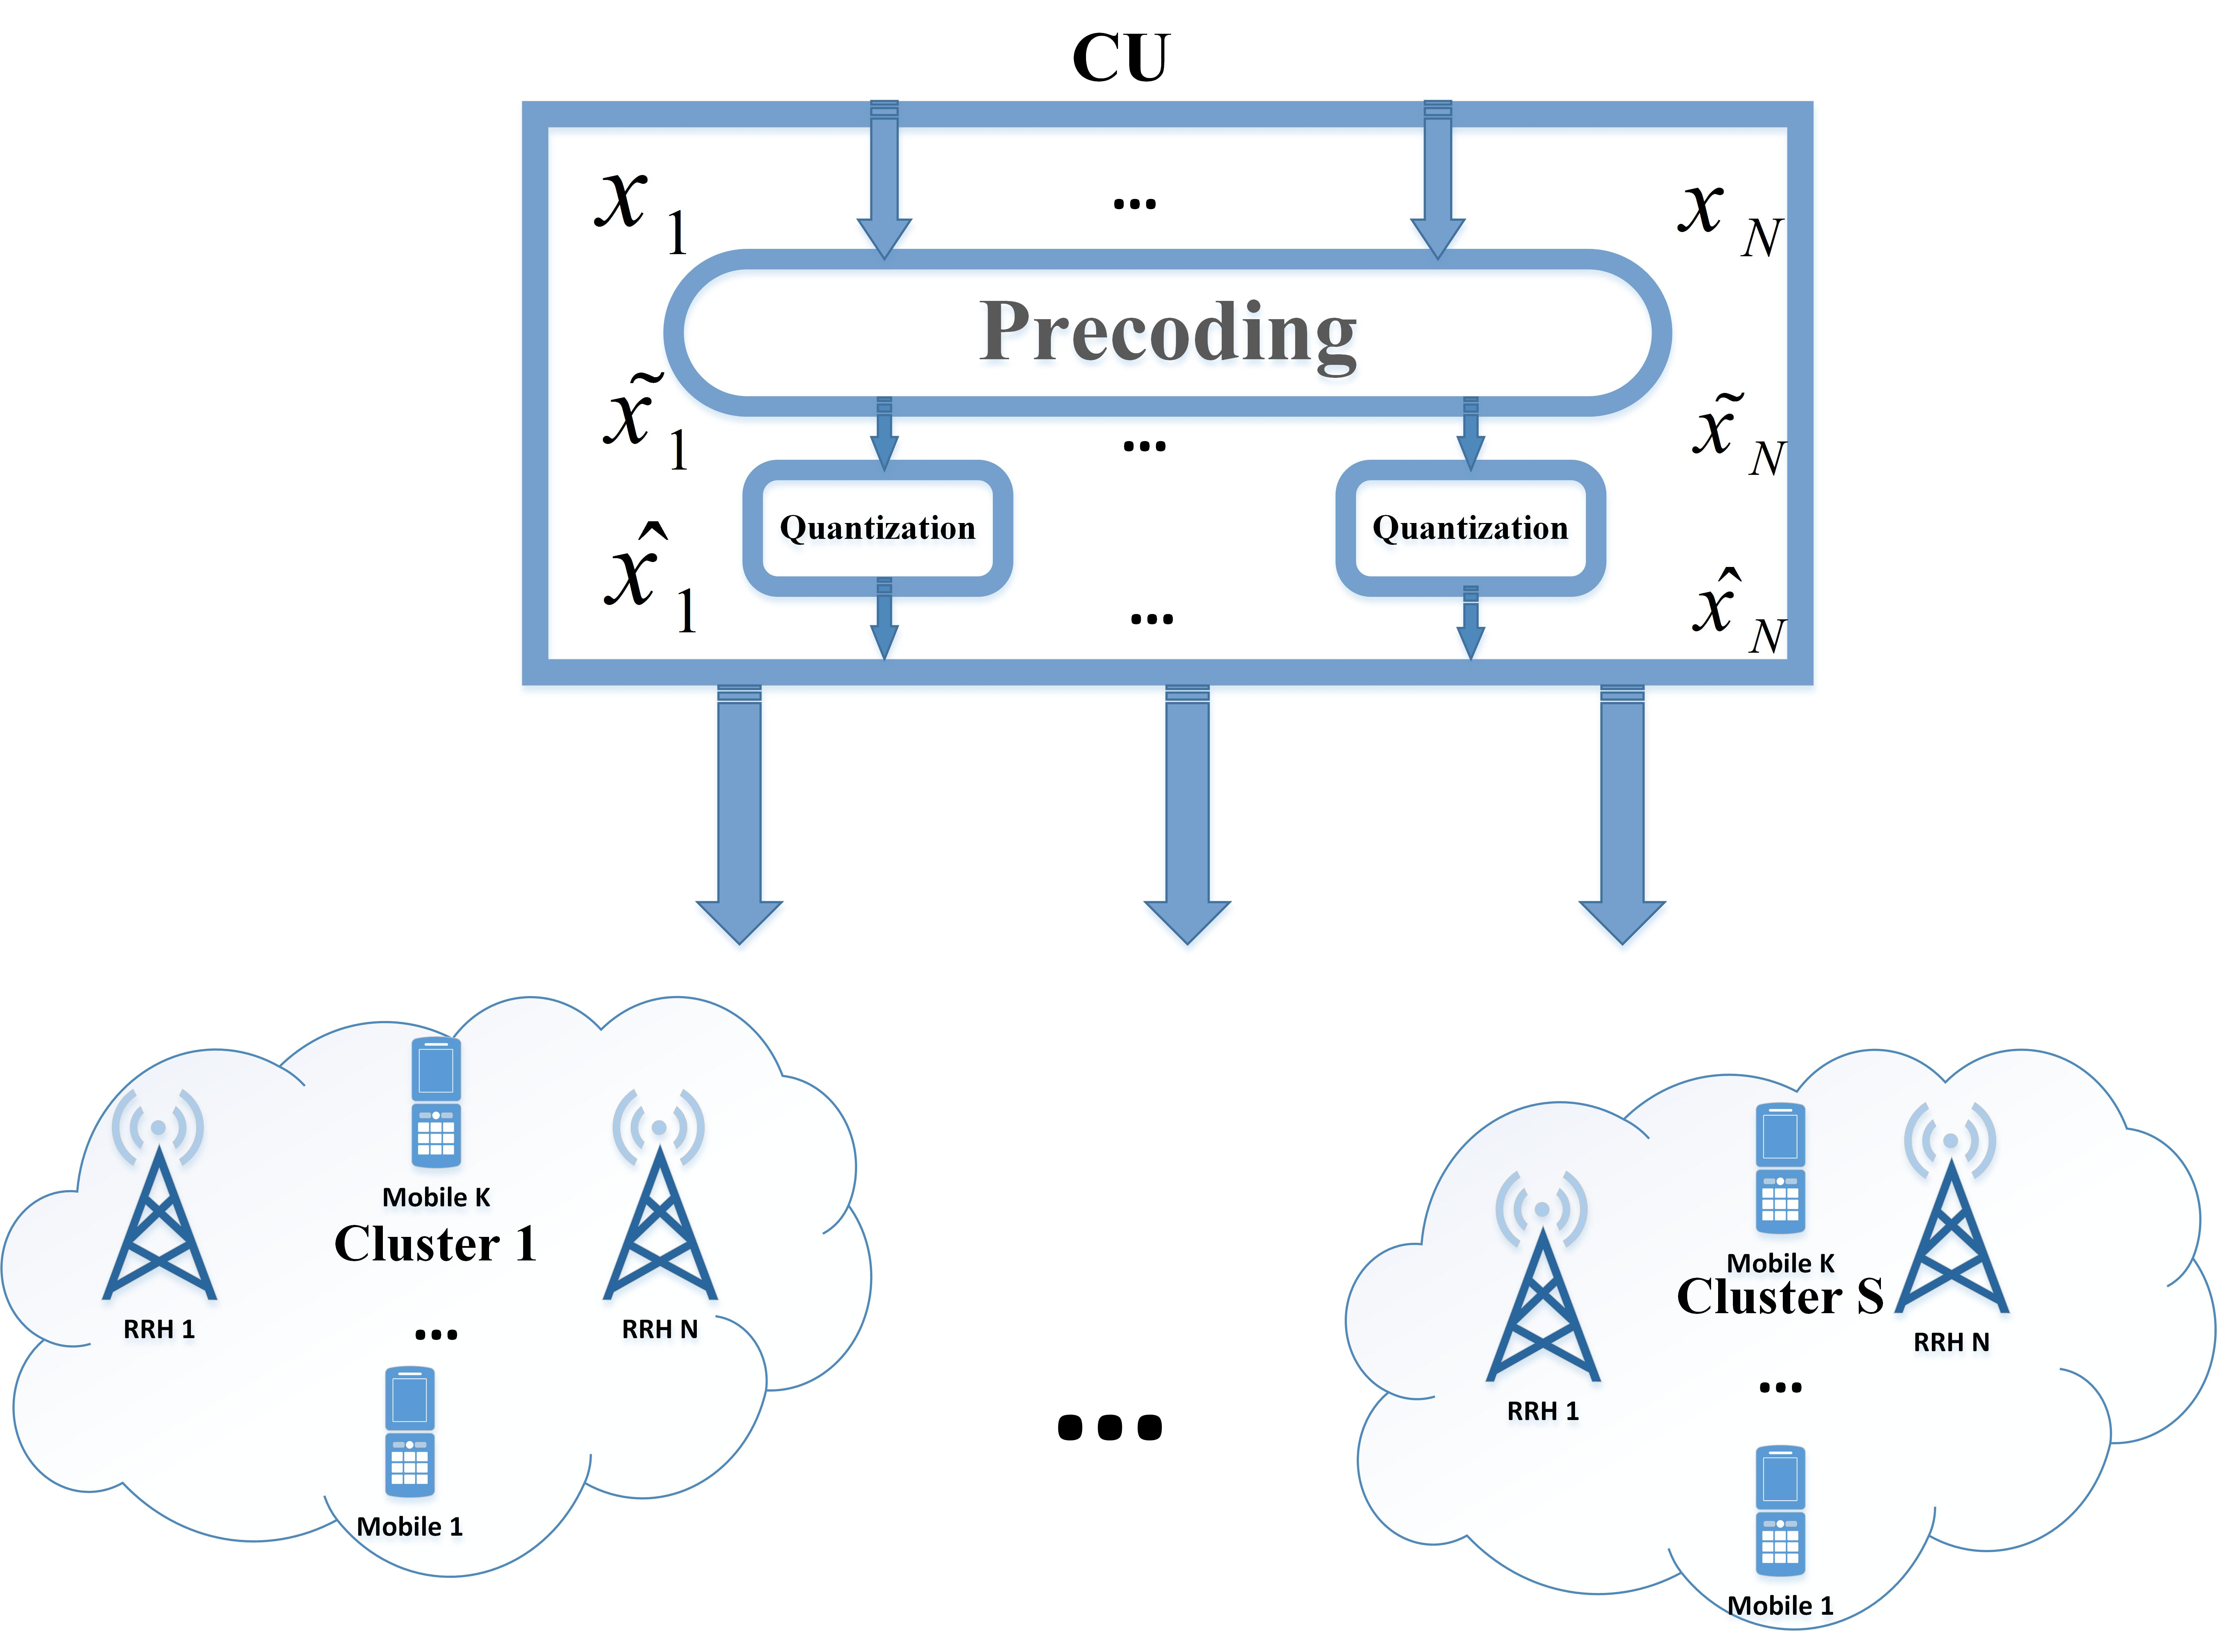
\includegraphics[width=\linewidth]{./fig/mydraw1}
  \caption{ساختار 
  \lr{C-RAN}
  در  لینک فروسو.
  }
  \label{fig:cr1}
\end{figure}
 فرض مسئله بر این است که سیستم به صورت چند آنتنه (\lr{MIMO})  می باشد و ظرفیت \lr{Fronthaul} محدود است. همچنین، سیستم دارای چندین خوشه یا سلول که در هر خوشه، تعدادی  واحد رادیویی و تعدادی کاربر قرار دارد\cite{EEcluster,jcluster}. هدف، بدست آوردن بیشینه بازدهی انرژی می باشد.\newline
 در حالت لینک فروسو، پیام، پیش کدگذاری شده است و سپس فشرده سازی بر روی آن صورت گرفته است و از طریق لینک \lr{Fronthaul} به واحد رادیویی منتقل می شود تا پیام را به کاربران ارسال کنند \cite{Fronthaul, ulSimeone, precodSimeone}
 .\newline
 در حالت لینک فراسو، سیگنال از کاربران به واحدهای رادیویی منتقل شده و سپس پیام فشرده شده و به دست واحد کنترل می رسد؛ تا با استفاده از روش های ترکیب کردن \LTRfootnote{combining}، پیام ارسالی کاربران بازیابی شود. 

\section{لینک فروسو}
در این بخش، لینک فروسو برای سیستم \lr{MIMO C-RAN} در نظر گرفته شده است که واحد کنترل، پیام را پیش کدگذاری کرده سپس سیگنال پیش کدگذاری شده را فشرده می کند. سیگنال فشرده شده ی نهایی توسط لینک \lr{Fronthaul} با ظرفیت محدود منتقل می گردد
\cite{dlsnr}.
\newline
فرض بر این است که واحدهای رادیویی و کاربران خوشه بندی شده اند به طوری که در هر خوشه تعدادی واحد رادیویی است که به کاربران موجود در آن خوشه، سرویس دهی می کنند.\newline
در این سیستم، فرستنده می بایست اطلاعات حالت کانال را بداند
(\lr{CSIT}). 
 از آنجایی که \lr{CSIT} با کمی خطا با ارسال پایلوت در لینک فراسو بدست می آید، به همین دلیل فرض در اینجا به این صورت است که تخمین \lr{CSIT}، همراه با خطای مشخص است. در واحد کنترل، از پیش کدگذاری از نوع \lr{MMSE} برای کاهش تداخل بین کاربران و بهبود عملکرد سیستم استفاده می گردد.\newline
همچنین، ابتدا نرخ قابل دسترسی را با توجه به ظرفیت محدود \lr{Fronthaul}، بدست می آوریم. سپس توان تخصیص داده را بهینه می کنیم تا \lr{EE} به مقدار بهینه ی خود برسد.\newline
در ادامه، ابتدا مدل سیستم و سپس نرخ قابل دسترسی بیان شده و مسئله ی تخصیص توان بررسی می گردد\cite{mkm}.
\subsection{مدل سیستم}
لینک فروسو سیستم \lr{MIMO C-RAN} شامل $R$  واحد رادیویی می باشد که $D$ کاربر تک آنتنه را سرویس می دهند.فرض بر این است که کاربران و واحدهای رادیویی، به 
 $S$
 تا خوشه تقسیم شده اند که $v$ امین خوشه،
 دارای $R_v$ واحد رادیویی است که ${D}_v$ کاربر را سرویس دهی می کنند\cite{EEcluster}.
 همچنین، فرض بر این است که
$j$
امین واحد رادیویی، در $v$امین خوشه، توسط لینک فیبر نوری با ظرفیت محدود $c_{r_{(v,j)}}$ به \lr{CU} متصل می گردد. در نتیجه داریم:
\begin{equation}
\begin{split}
\mathcal{R}_v= \{  r_{(v,i)} | 1 \leq i \leq {R}_v , i\in Z^+\}, \\
\mathcal{C}_{\mathcal{R}_v}= \{C_{r_{(v,j)}}| 1 \leq j \leq {R}_v , j\in Z^+\}, \\
\mathcal{D}_v= \{  d_{(v,k)} | 1 \leq k \leq {D}_v , k\in Z^+\},  \\
\end{split}
\end{equation} 
که
 $\mathcal{R}_v$، $\mathcal{C}_{\mathcal{R}_v}$
 و
  $\mathcal{D}_v$
 به ترتیب نشان دهنده ی دسته ی واحدهای رادیویی، دسته ی ظرفیت لینک \lr{Fronthaul} و دسته ی کاربران در $v$امین دسته ی خوشه می باشد.\newline
در واحد کنترل، ما روش فشرده سازی بعد از پیش کدگذاری و سپس ارسال را اعمال کرده ایم. هر کاربر همزمان تداخل بین خوشه ها و داخل یک خوشه را همزمان دریافت می کنند.
 \subsection{آنالیز نرخ قابل دسترس}
در این زیربخش، نرخ قابل دسترسی سیستم بررسی می گردد.
\begin{theorem}\label{t1}
 نرخ قابل دسترسی برای کاربر $d_{(s,k)}$ به صورت زیر می باشد:
\begin{equation}\label{e1}
\mathfrak{R}_{d_{(s,k)}} = B \log_2(1+\gamma_{d_{(s,k)}}),
\end{equation}
که $B$ پهنای باند کانال و $\gamma_{d_{(s,k)}}$ همان \lr{SINR} دریافتی $k$امین کاربر در $s$امین دسته ی خوشه است که به صورت زیر بیان می گردد.  
\begin{equation}\label{5}
\gamma_{d_{(s,k)}}= \frac{p_{d_{(s,k)}}|\boldsymbol{h}_{\mathcal{R}_s, d_{(s,k)}}^H \boldsymbol{w}_{\mathcal{R}_{s},d_{(s,k)}}|^2}{I_{d_{(s,k)}}+BN_0}.
\end{equation}
در فرمول \eqref{5}، 
$I_{d_{(s,k)}}$
نشان دهنده ی توان سیگنال تداخلی است.$BN_0$
نشان دهنده ی توان نویز است و
$\boldsymbol{h}_{\mathcal{R}_s, d_{(s,k)}}$ 
 نشان دهنده ی بردار کانال بین $k$امین کاربر و واحدهای رادیویی
 $s$
 امین دسته ی خوشه می باشد. همچنین 
 $\boldsymbol{w}_{\mathcal{R}_{s},d_{(s,k)}}$
 نشان دهنده ی بردار پیش کدگذاری استفاده شده در $s$امین دسته ی خوشه ها برای $k$امین کاربر می باشد. 
 $p_{d_{(s,k)}}$
 توان ارسالی واحدهای رادیویی است که به $k$امین کاربر در $s$امین دسته ی خوشه ارسال می گردد.
\end{theorem}
\begin{proof}
فرض کنید $\boldsymbol{y}_{\mathcal{D}_s}$ یک بردار
 $D_s \times 1$
باشد که نشان دهنده ی سیگنال دریافتی توسط دسته ای از کاربران در $s$
امین خوشه باشد که به صورت زیر بدست می آید.
\begin{equation} \label{1}
\boldsymbol{y}_{\mathcal{D}_s} = \sum_{v=1}^S \boldsymbol{H}^H_{\mathcal{R}_v,\mathcal{D}_s}\hat{\boldsymbol{x}}_{\mathcal{R}_v}+ \boldsymbol{z}_{\mathcal{D}_s},
\end{equation}
که   $\hat{\boldsymbol{x}}_{ \mathcal{R}_v} = [\hat{x}_{ r_{(v,1)}},...,\hat{ x}_{ r_{(v,\mathcal{R}_v)}}]^T \in \mathbb{C}^{{R}_v } $ 
بردار سمبل ارسالی خوشه ی  $v$ ام می باشد.\newline
 $\boldsymbol{z_{\mathcal{D}_s}} \backsim \mathcal{N}(0,N_0\boldsymbol{I}_{{D}_s})$ 
 نویز گوسی سفید اضافه شونده می باشد که دارای توان $N_0$
 و 
 $\boldsymbol{H}_{\mathcal{R}_v,\mathcal{D}_s}=\left[\boldsymbol{h}_{\mathcal{R}_v,d_{(s,1)}},\ldots,\boldsymbol{h}_{\mathcal{R}_v,d_{(s,\mathcal{D}_s)}}\right]^T  \in \mathbb{C}^{{R}_v\times {D}_s}$ 
 نشان دهنده ی ماتریس کانال بین واحدهای رادیویی دسته ی $\mathcal{R}_v$ و کاربران $\mathcal{D}_s$ می باشد.
 بردار کانال از واحدهای رادیویی خوشه ی  $v$ به $k$ امین کاربر در خوشه ی $s$ام  
 $\boldsymbol{h}_{\mathcal{R}_v,d_{(s,k)}}\in \mathbb{C}^{{R}_v}$
 به صورت زیر مدل می شود \cite{cellfree}
 \begin{equation}\label{channel}
\boldsymbol{h}_{\mathcal{R}_v,d_{(s,k)}} = \boldsymbol{\beta}^\frac{1}{2}_{\mathcal{R}_v,d_{(s,k)}} \boldsymbol{g}_{\mathcal{R}_v,d_{(s,k)}},
\end{equation}
% resizebox{0.3\hsize}{!}{$
که  $\boldsymbol{g}_{\mathcal{R}_v,d_{(s,k)}} \backsim \mathcal{N}(0,N_0\boldsymbol{I}_{\mathcal{D}_s})$ نشان دهنده ی بردار کانال محو شدگی سریع و مسطح می باشد 
و $\boldsymbol{\beta}_{\mathcal{R}_v,d_{(s,k)}}=\text{\lr{diag}}(a_{r_{(v,1),d_{(s,k)}}},\ldots,a_{r_{(v,\mathcal{R}_v),d_{(s,k)}}})$
نشان دهنده ی محوشدگی  در مقیاس بزرگ می باشد. همچنین سیگنال ارسالی تحت فشرده سازی به صورت زیر است
\begin{equation}
\label{eq_pow1}
 \hat{\boldsymbol{x}}_{\mathcal{R}_v} = \tilde{\boldsymbol{x}}_{\mathcal{R}_v} + \boldsymbol{Q}_{\mathcal{R}_v},
\end{equation}

که در اینجا $\boldsymbol{Q}_{\mathcal{R}_v} = \left[ q_{r_{(v,1)}},\ldots,q_{r_{(v,R_v)}}\right]^T$ نشان دهنده ی بردار نویز کوانتیزاسیون می باشد که به دلیل فشرده سازی بعد از پیش کدگذاری در واحد کنترل ایجاد می گردد که دارای توزیع $q_{M_{(t,i)}}\backsim \mathcal{N}(0,\sigma_{q_{(t,i)}}^2) $ است.
علاوه بر این،  
$$\tilde{\boldsymbol{x}}_{\mathcal{R}_v} = \textbf{\lr{W}}_{\mathcal{R}_v,\mathcal{D}_v} \textbf{\lr{P}}_{\mathcal{D}_v}^{\frac{1}{2}} \boldsymbol{x}_{ \mathcal{D}_v},$$
نشان دهنده ی پیام پیش کدگذاری شده قبل از فشرده سازی می باشد.
همانطور که گفته شده بود، فرض بر این است که بردار کانال را می دانیم و همراه با خطا بدست آمده است؛ کانال همراه با خطا به صورت زیر مدل شده است: 
\begin{equation*}
\hat{\boldsymbol{h}}_{\mathcal{R}_v,d_{(s,k)}} = \boldsymbol{h}_{\mathcal{R}_v,d_{(s,k)}} + \Delta \boldsymbol{h}_{\mathcal{R}_v,d_{(s,k)}},
\end{equation*}

$\Delta \boldsymbol{h}_{\mathcal{R}_v,d_{(s,k)}}$
نشان دهنده ی بردار خطای تخمین زده شده است که دارای توزیع گوسی به صورت
$$\Delta \boldsymbol{h}_{\mathcal{R}_v,d_{(s,k)}}\backsim \mathcal{N}(0,\boldsymbol{\phi}_{\mathcal{R}_v,d_{(s,k)}}^2),$$
است که  داریم 
$$\boldsymbol{\phi}_{\mathcal{R}_v,d_{(s,k)}} = \text{\lr{diag}}(\phi_{r_{(v,1)},d_{(s,k)}},\ldots,\phi_{r_{(v,\mathcal{R}_v)},d_{(s,k)}}).$$
با استفاده از پیش کدگذاری \lr{MMSE}، ماتریس پیش کدگذاری به صورت زیر است \cite{digCom}
\begin{equation}
\boldsymbol{W}_{\mathcal{R}_s,\mathcal{D}_s} = \hat{\boldsymbol{H}}_{\mathcal{R}_s,\mathcal{D}_s}(\hat{\boldsymbol{H}}_{\mathcal{R}_s,\mathcal{D}_s}^H \hat{\boldsymbol{H}}_{\mathcal{R}_s,\mathcal{D}_s}+ \alpha \boldsymbol{I}_{{D}_s})^{-1},
\end{equation} 
همچنین  $\alpha$، فاکتور رگولاریزاسیون است
بنابراین، $I_{d_{(s,k)}}$ را که توان تداخلی بر روی کاربر بود به صورت زیر می توان تخمین زد.
\begin{equation}\label{6}
\begin{split}
I_{d_{(s,k)}} &=  \underbrace{\sum_{\substack{l=1 \\ l\neq k}}^{{D}_s} |\boldsymbol{h}_{\mathcal{R}_s, d_{(s,k)}}^H \boldsymbol{w}_{\mathcal{R}_{s},d_{(s,l)}}|^2  p_{d_{(s,l)}}}_{\text{(\lr{intra-cluster interference})}}\\
&+\underbrace{\sum_{\substack{v=1 \\ v\neq s}}^{S} \sum_{l=1}^{{D}_v} |\boldsymbol{h}_{\mathcal{R}_v, d_{(s,k)}}^H \boldsymbol{w}_{\mathcal{R}_{v},d_{(v,l)}}|^2 p_{d_{(v,l)}}}_{\text{(\lr{inter-cluster interference})}}\\
& +\underbrace{ \sum_{v=1}^{S} \sum_{i=1}^{{R}_v} {\sigma_q}_{r_{(v,i)}}^2  |h_{r_{(v,i)}, d_{(s,k)}}|^2 }_{\text{(\lr{quantization noise interference})}}.
\end{split}
\end{equation}
\end{proof}
\subsection{بهینه سازی تخصیص توان}
می دانیم که توان سیگنال ارسالی توسط  $i$امین واحد رادیویی در $s$امین خوشه  به صورت زیر می باشد : 
\begin{equation} \label{eq_pow2}
\bar{p}_{r_{(s,i)}} = \mathit{E}[|| \hat{x}_{\mathcal{D}_v} ||^2],
\end{equation}

با قرار دادن رابطه ی  (\ref{eq_pow1}) در (\ref{eq_pow2})، توان سیگنال ارسالی به این صورت بدست می آید:
\begin{equation}
\bar{p}_{r_{(s,i)}} = \boldsymbol{w}_{r_{(s,i)},\mathcal{D}_{s}} \boldsymbol{P}_{\mathcal{D}_s}^{\frac{1}{2}} \boldsymbol{P}_{\mathcal{D}_s}^{H \frac{1}{2}}   \boldsymbol{w}_{r_{(s,i)},\mathcal{D}_{s}}^H + \sigma_{q_{(s,i)}}^2.
\end{equation}
در نتیجه نرخ قابل دسترس بر روی لینک \lr{fronthaul}، بین واحد کنترل و $i$امین واحد رادیویی در $t$امین خوشه  به صورت زیر بدست می آید 
\begin{equation}
C_{r_{(t,i)}} = \log{(1+\frac{\boldsymbol{w}_{r_{(s,i)},\mathcal{D}_{s}} \boldsymbol{P}_{\mathcal{D}_s}^{\frac{1}{2}} \boldsymbol{P}_{\mathcal{D}_s}^{H \frac{1}{2}}   \boldsymbol{w}_{r_{(s,i)},\mathcal{D}_{s}}^H }{ \sigma_{q_{(s,i)}}^2})},
\end{equation}
\subsubsection{شرح مسئله}
نسبت مجموع نرخ ها در سیستم به کل توان ارسالی واحدهای رادیویی نشان دهنده ی بازدهی انرژی است که یکی از مهم ترین پارامترها در انتخاب تکنولوژی می باشد که با $\eta$ نمایش داده می شود و می توان اینگونه بیان کرد
\begin{equation}\label{eta}
\eta(\boldsymbol{P}) := \frac{\sum\limits_{s=1}^{S} \sum\limits_{k=1}^{{D}_s}\mathfrak{R}_{d_{(s,k)}} }{\sum\limits_{s=1}^{S} \sum\limits_{i=1}^{{R}_s}\bar{p}_{r_{(s,i)}}} = \frac{R_{total}(\boldsymbol{P})}{P_{RRH}(\boldsymbol{P})},
\end{equation}
که در اینجا  $ \boldsymbol{P} = \{ \boldsymbol{P}_{\mathcal{D}_s}|  1 \leq s \leq S, s \in \mathbb{Z}^{+} \}$ ماتریس تخصیص توان است. در این بخش، بیشینه سازی بازدهی انرژی با شروط زیر مورد بررسی قرار می گیرد 
\begin{equation}\label{p1}
\begin{aligned}
\max\limits_{\boldsymbol{P}}   \quad &   \eta(\boldsymbol{P})\\
\text{\lr{subject to}} \quad  & \bar{p}_{r_{(s,i)}} \leq P_{max} && \qquad \forall s, \forall i,   \\
&\mathfrak{R}_{d_{(s,k)}} \geq  \mathfrak{R}_{d_{(s,k)}}^{th} && \qquad \forall s, \forall k, \\
&C_{r_{(s,i)}} \leq C_{r_{(s,i)}}^{th}  &&\qquad \forall s, \forall i, \\
&p_{d_{(s,k)}}  \geq 0                                  &&\qquad \forall s, \forall k, \\
\end{aligned}			
\end{equation}
از آنجایی که این یک مسئله ی محدب نیست، با روش الگوریتم تکرار شونده ، مقدار توان بهینه را بدست می آوریم\cite{boyd}.
\subsection{روش مورد استفاده}
در این قسمت، به جای ماکسیمم کردن \eqref{eta}، مسئله ی معادل آن را با الگوریتم تکرار شونده حل می کنیم
\begin{theorem}\label{t2}
مقدار ماکسیمم $\eta^*$  تنها زمانی بدست می آید که
\begin{equation}\label{q2}
\begin{split}
&\max \limits_{\boldsymbol{P}} (R_{total}(\boldsymbol{P}) - \eta^* P_{RRH}(\boldsymbol{P}))=\\
& R_{total}(\boldsymbol{P}^*) - \eta^* P_{RRH}(\boldsymbol{P}^*) =0,
\end{split}
\end{equation}
که $\{\boldsymbol{P}\}$  یک پاسخ امکان پذیر برای مسئله ی \eqref{p1} باشد \cite{hcranEE}.
\end{theorem}
\begin{proof}
اثبات این قضیه با روش مشابه در مقاله ی \cite{hcranEE} حل شده است.
\end{proof}

برای حل مسئله ی بهینه سازی \eqref{q2}، از تابع لاگرانژ استفاده می کنیم \cite{boyd} که توسط الگوریتم تکرار شونده بدست می آید. برای ساده سازی کران بالا برای تداخل  \eqref{6}، به این صورت بدست می آید
\begin{equation}
\begin{split}
\tilde{I}_{d_{(s,k)}} &= \sum_{v=1}^{S} P_{max}|| \boldsymbol{h}_{\mathcal{R}_v,d_{(s,k)}} \boldsymbol{w}_{\mathcal{R}_v,d_{(s,k)}}||^2 ,\\
& +  \sum_{v=1}^{S} \sum_{i=1}^{{R}_v} {\sigma_q}_{r_{(v,i)}}^2  |h_{r_{(v,i)}, d_{(s,k)}}|^2.
\end{split}
\end{equation}
بنابراین، برای بدست آوردن توان بهینه کران پایینی برای نرخ بدست می آید
\begin{equation}\label{e11}
\mathfrak{\tilde{R}}_{d_{(s,k)}} = B \log_2(1+\tilde{\gamma}_{d_{(s,k)}}),
\end{equation}
که  $\tilde{\gamma}_{d_{(s,k)}}$ به صورت زیر است 
\begin{equation}\label{15}
\tilde{\gamma}_{d_{(s,k)}} =  \frac{p_{d_{(s,k)}}|\boldsymbol{h}_{\mathcal{R}_s, d_{(s,k)}}^H \boldsymbol{w}_{R_{s},d_{(s,k)}}|^2}{\tilde{I}_{d_{(s,k)}}+BN_0};
\end{equation}

همانطور که قبلا بیان شد، الگوریتم تکرار شونده برای بهینه سازی مورد استفاده قرار می گیرد که براساس ضرایب تابع لاگرانژ می باشد 
\begin{equation}
\begin{split}
\mathcal{L}(\boldsymbol{P}; \boldsymbol{\lambda}, \boldsymbol{\mu}, \boldsymbol{ \kappa}) & = \sum\limits_{s=1}^{S} \sum\limits_{k=1}^{\mathcal{D}_s}\mathfrak{\tilde{R}}_{d_{(s,k)}} 
- \eta \sum\limits_{s=1}^{S} \sum\limits_{i=1}^{\mathcal{R}_s}\bar{p}_{r_{(s,i)}}\\
&+\sum\limits_{s=1}^{S} \sum\limits_{k=1}^{\mathcal{D}_s} \lambda_{d_{(s,k)}} (\mathfrak{\tilde{R}}_{d_{(s,k)}}-\mathfrak{R}_{d_{(s,k)}}^{th})\\
&- \sum\limits_{s=1}^{S} \sum\limits_{i=1}^{\mathcal{R}_s} \mu_{r_{(s,i)}} (\bar{p}_{r_{(s,i)}}-P_{max})\\
&- \sum\limits_{s=1}^{S} \sum\limits_{i=1}^{\mathcal{R}_s} \kappa_{r_{(s,i)}} (C_{r_{(s,i)}}-C_{r_{(s,i)}}^{th}).\\
\end{split}
\end{equation}
که در اینجا، $\boldsymbol{\lambda}, \boldsymbol{\mu}, \boldsymbol{\kappa} \geq 0$
بردارهای ضرایب لاگرانژ می باشد .\newline
با استفاده از این معادله، توان بهینه به صورت زیر بدست می آید
\begin{equation}
p_{d_{(s,k)}}^* =[\frac{ B(1+\lambda_{d_{(s,k)}} )}{\ln2 \times (\iota_{d_{(s,k)}}+ \chi_{d_{(s,k)}})} -\frac{\tilde{I}_{d_{(s,k)}} + BN_0}{\nu_{d_{(s,k)}} }]^+;
\end{equation} 
که داریم
 $$\nu_{d_{(s,k)}} =|h_{\mathcal{R}_s, d_{(s,k)}}^H \boldsymbol{w}_{R_{s},d_{(s,k)}}|^2,$$
 $$\iota_{d_{(s,k)}}= \sum\limits_{i=1}^{\mathcal{R}_s} (\mu_{r_{(s,i)}}+\eta)(w_{r_{(s,i)},d_{(s,k)}} w_{r_{(s,i)},d_{(s,k)}}^*),$$
 $$\chi_{r_{(s,i)}} \approx  \sum\limits_{i=1}^{\mathcal{R}_s} \frac{\kappa_{r_{(s,i)}}}{\ln 2}\frac{(w_{r_{(s,i)},d_{(s,k)}} w_{r_{(s,i)},d_{(s,k)}}^*)}{ P_{max}}.$$
  در آخر، برای بدست آوردن توان بهینه، الگوریتم \eqref{alg} مورد استفاده قرار می گیرد \cite{hcranEE}
 \begin{latin}
\begin{algorithm}
\caption{Energy-Efficient Power Allocation}\label{alg}
\begin{algorithmic}

\State Set the maximum number of iterations $I_{max}$, convergence condition $\epsilon_{\eta}$  and the initial value $\eta^{(1)} = 0$
\State Set the iteration index $i = 1$ and begin the iteration (Outer
Loop).
\For {$ 1\leq i \leq  Imax$}
\State Solve the resource allocation problem with $\eta^{(i)}$ (Inner Loop);
\State Obtain $P^{(i)}, R_{total}^{(i)}, P_{RRH}^{(i)}$
\If {$ R_{total}(\boldsymbol{P}^{(i)}) - \eta^{(i)} P_{RRH}(\boldsymbol{P}^{(i)}) < \epsilon_{\eta} $} 
\State Set $\boldsymbol{P}^*= \boldsymbol{P}^{(i)} $   and  $ \eta^{*} =\eta^{(i)} $;
\State break;
\Else
\State Set $\eta^{(i)}= \frac{R_{total}(\boldsymbol{P}^{(i))}}{P_{RRH}(\boldsymbol{P}^{(i))}}$ and $i= i+1$;
\EndIf 
\State \textbf{end if}
\EndFor 
\State \textbf{end for}

\end{algorithmic}
\end{algorithm}
\end{latin}
%%%%%%%%%%%%%%%%%%%%%%%%%%%%%
\subsection{نتایج عددی}
در این بخش، نتایج عددی الگوریتم مورد استفاده برای سیستم \lr{MIMO C-RAN} با پارامترهای بیان شده در جدول \ref{tab:title} بیان می شود.
\begin{latin} 
 \begin{table}[H]
 \caption {\rl{پارامترهای شبیه سازی}} \label{tab:title} 
 \begin{center}
  \begin{tabular}{||c c ||} 
  \hline
  Parameter & Value \\ [0.5ex] 
  \hline\hline
  Number of cluster S & 2 \\ 
  \hline
  Noise power density & -174dBm/Hz\\
  \hline
  Bandwidth & 120KHz \\
  \hline
 Maxmimun transmit Power & 23dBm \\
  \hline
  Circuit Power of whole RRHs & 10dBm \\
  \hline
  Variance of quantization noise & $10^{-4}$ \\
  \hline
   Maxmimun fronthaul link's rate & 5bits/sec/Hz \\
  \hline
  Minimum data rate &  1bits/sec/Hz \\ [1ex] 
  \hline
 \end{tabular}
 \end{center}
 \end{table}
 \end{latin}
  \begin{figure}[h]
  \centering
    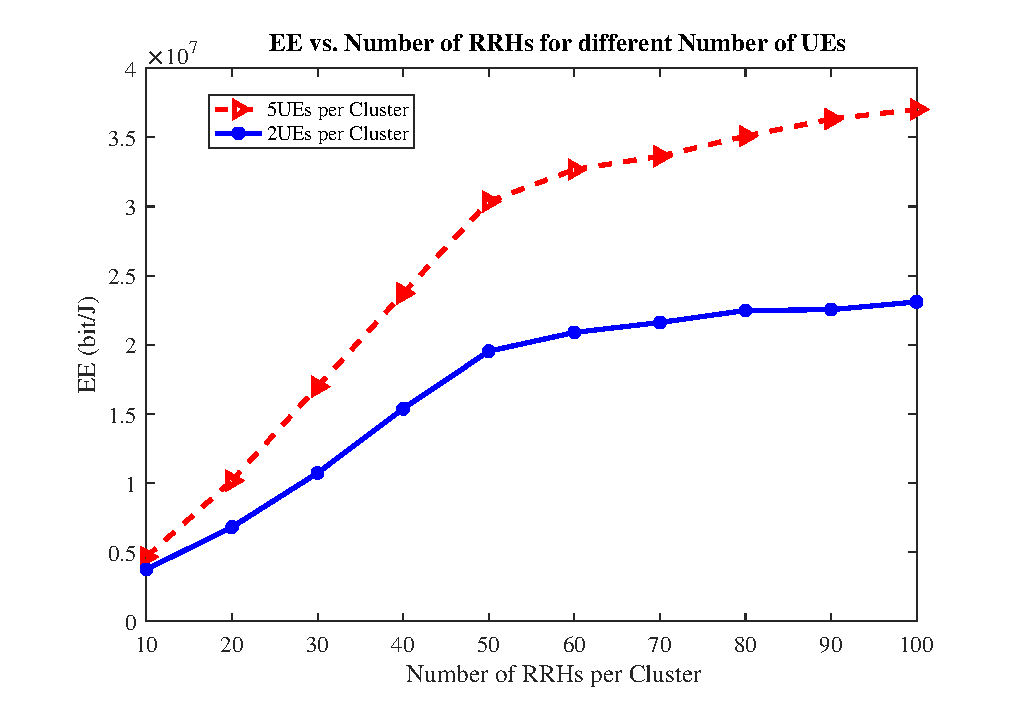
\includegraphics[width=\linewidth, height=12cm]{./fig3/rrh}
  \caption{
  بازدهی انرژی با توجه به تغییرات تعداد واحدهای رادیویی در هر خوشه برای توان بهینه برای 
   دو کاربر مختلف
   و پارامترهای جدول \ref{tab:title}}
  \label{fig:nem1}
\end{figure}
 در شکل \ref{fig:nem1}، بازدهی انرژی سیستم \lr{MIMO C-RAN} بر اساس تعداد واحدهای رادیویی در هر خوشه برای الگوریتم مورد استفاده و برای دو تعداد کاربر متفاوت، رسم شده است. 
 همانطور که  شکل  نشان می دهد، با افزایش تعداد واحدهای رادیوی، بازدهی انرژی افزایش می یابد و سپس  در این شکل از حدود 50 واحد رادیویی شیب افزایش بازدهی انرژی کمتر شده و به نظر می آید که رو به ثابت شدن است زیرا با افزایش واحد های رادیویی ابتدا نرخ ارسال داده بیشتر می شود و بازدهی انرژی بهبود می یابد و در نهایت نرخ ارسال داده دیگر بیشتر نمی گردد و ثابت می شود. زیرا در اینجا با افزایش تعداد واحدهای رادیویی، مجموع توان کل افزایش می یابد در نتیجه نرخ انتقال داده نیز بیشتر می گردد.

  \begin{figure}[h]
  \centering
    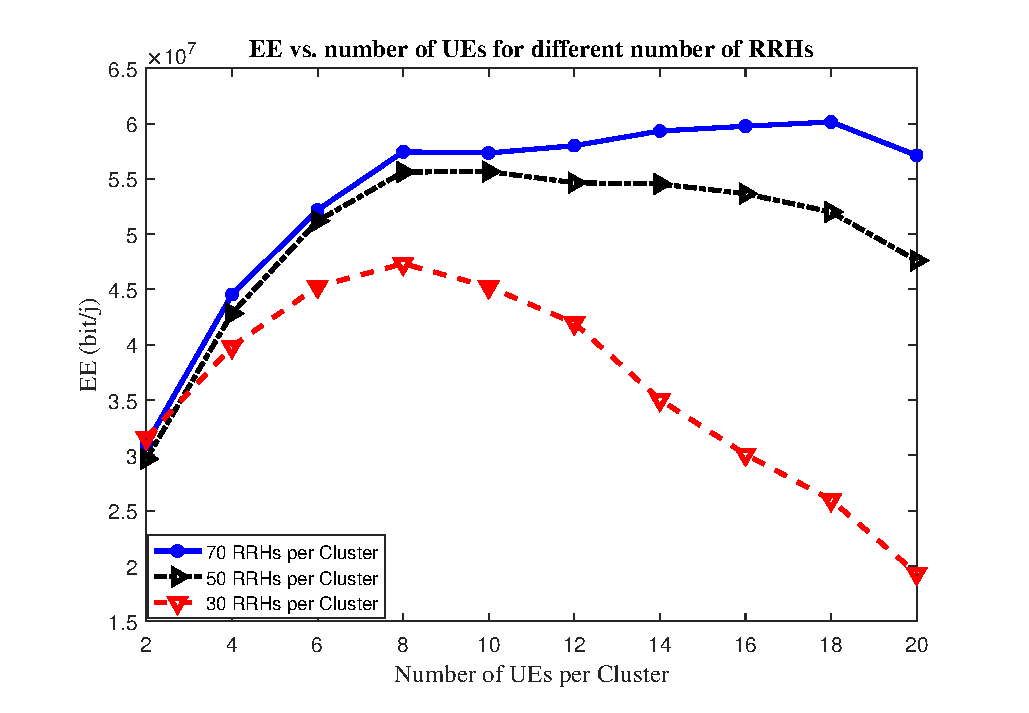
\includegraphics[width=\linewidth]{./fig3/ueEnd}
  \caption{  بازدهی انرژی با توجه به تغییرات تعداد کاربران در هر خوشه برای توان بهینه  برای 
   سه واحد رادیویی مختلف
   و پارامترهای جدول \ref{tab:title} و $P_c = 9dbm$}
  \label{fig:nem2}
\end{figure}


در شکل \ref{fig:nem2}، بازدهی انرژی بر اساس تعداد کاربران در هر خوشه برای الگوریتم مورد استفاده و برای سه تعداد واحد رادیویی متفاوت، رسم شده است.همانطور که  دیده می شود با افزایش تعداد کاربران، ابتدا شیب نمودار زیاد می شود و بازدهی انرژی افزایش می یابد زیرا با افزایش کاربران مجموع نرخ های انتقال افزایش می یابد ولی از یک مقدار به بعد تداخل بین کاربران افزایش می یابد و تاثیر خودر را به طور محسوس بر بازدهی انرژی می گذارد و در نتیجه بازدهی انرژی کاهش می یابد. 

%\bibliographystyle{ieeetr}
%\bibliography{bib1}
%\setLTRbibitems
\begin{figure}[H]
  \centering
    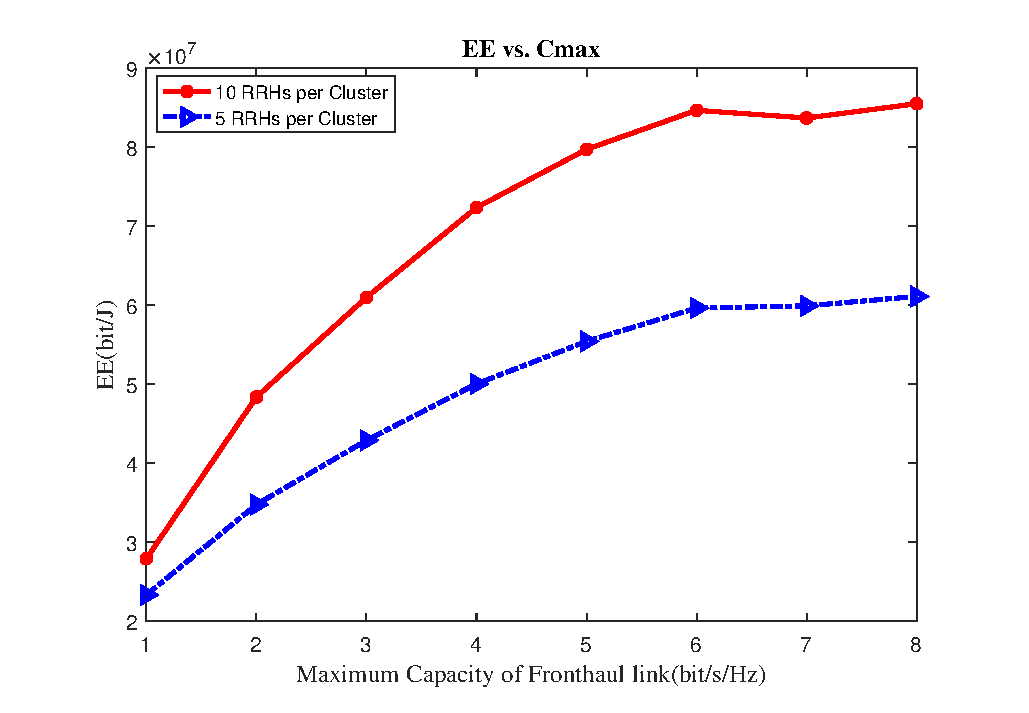
\includegraphics[width=\linewidth]{./fig3/cm}
  \caption{  بازدهی انرژی با توجه به تغییرات $C^{th}$، در در حالت $S =2$, $\text{\lr{Number of RRHs per Cluster}} = 10 , 5$, $\text{\lr{Number of UE per Cluster}} =2$ }
  \label{fig:nem3}
\end{figure}

در شکل \ref{fig:nem3}، بازدهی انرژی بر اساس محدودیت ظرفیت لینک \lr{fronthaul}، برای دو تعداد متفاوت  5 و 10 واحد رادیویی در هر خوشه رسم شده است. با توجه به شکل، زمانی که ظرفیت یک مقداری بیشتر
 می گردد، بدلیل اینکه نرخ قابل دسترس توسط تعداد کاربران و واحدهای رادیویی محدود می گردد، به نظر می آید افزایش محدودیت این ظرفیت تاثیر چندانی در بازدهی انرژی ندارد.  

% \begin{figure}[H]
%  \centering
%    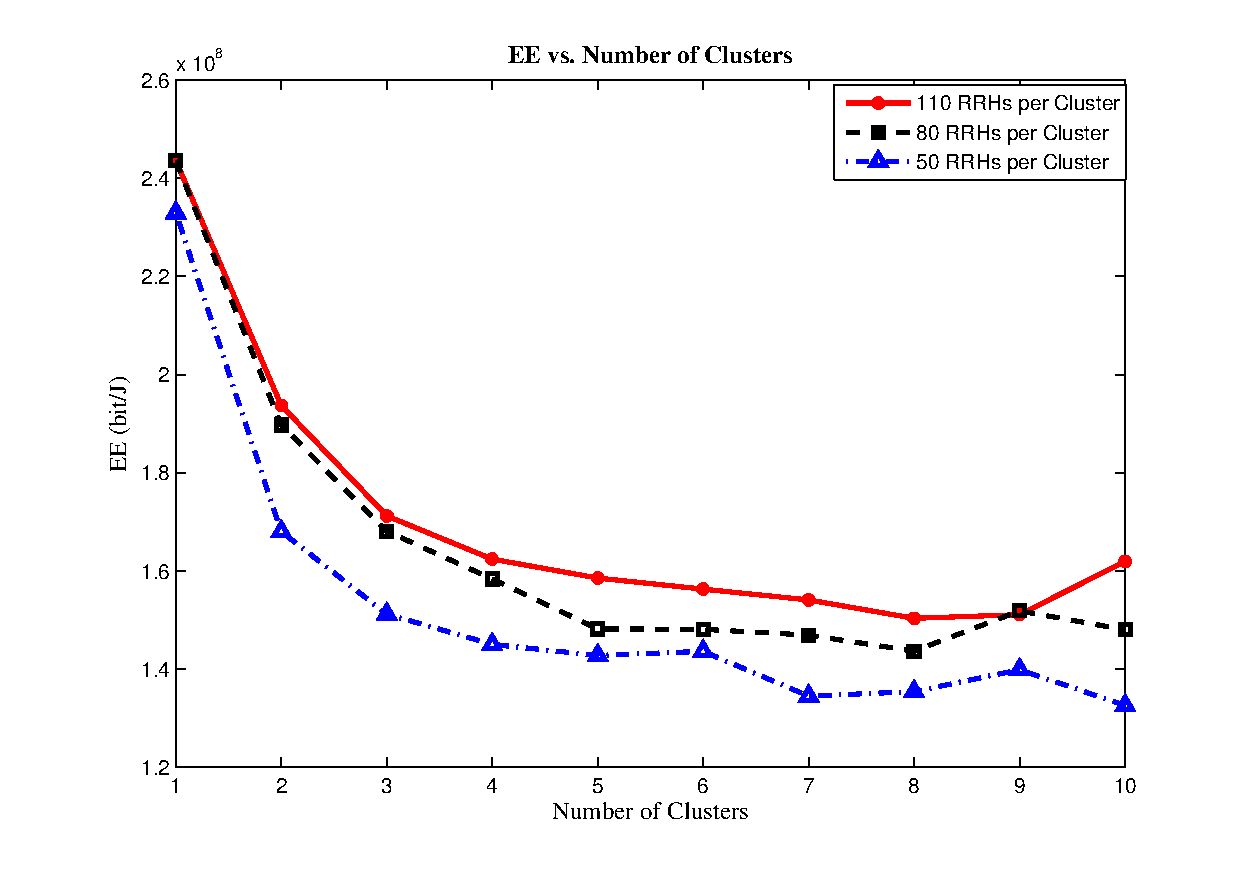
\includegraphics[width=\linewidth]{./fig3/clust}
%  \caption{  بازدهی انرژی بر حسب تعداد خوشه ها برای سه مقدار 50 و 80 و 110 واحد رادیویی}
%  \label{fig:cluster}
%\end{figure}
% حال در شکل \ref{fig:cluster}، بازدهی انرژی بر حسب تعداد خوشه ها برای سه مقدار 50 و 80 و 110 واحد رادیویی در هر خوشه با فرض وجود 3 کاربر در هر خوشه رسم شده است. همانطور که می بینید با افزایش خوشه ها بازدهی انرژی کاهش یافته است.
% 
 
 \begin{figure}[H]
  \centering
    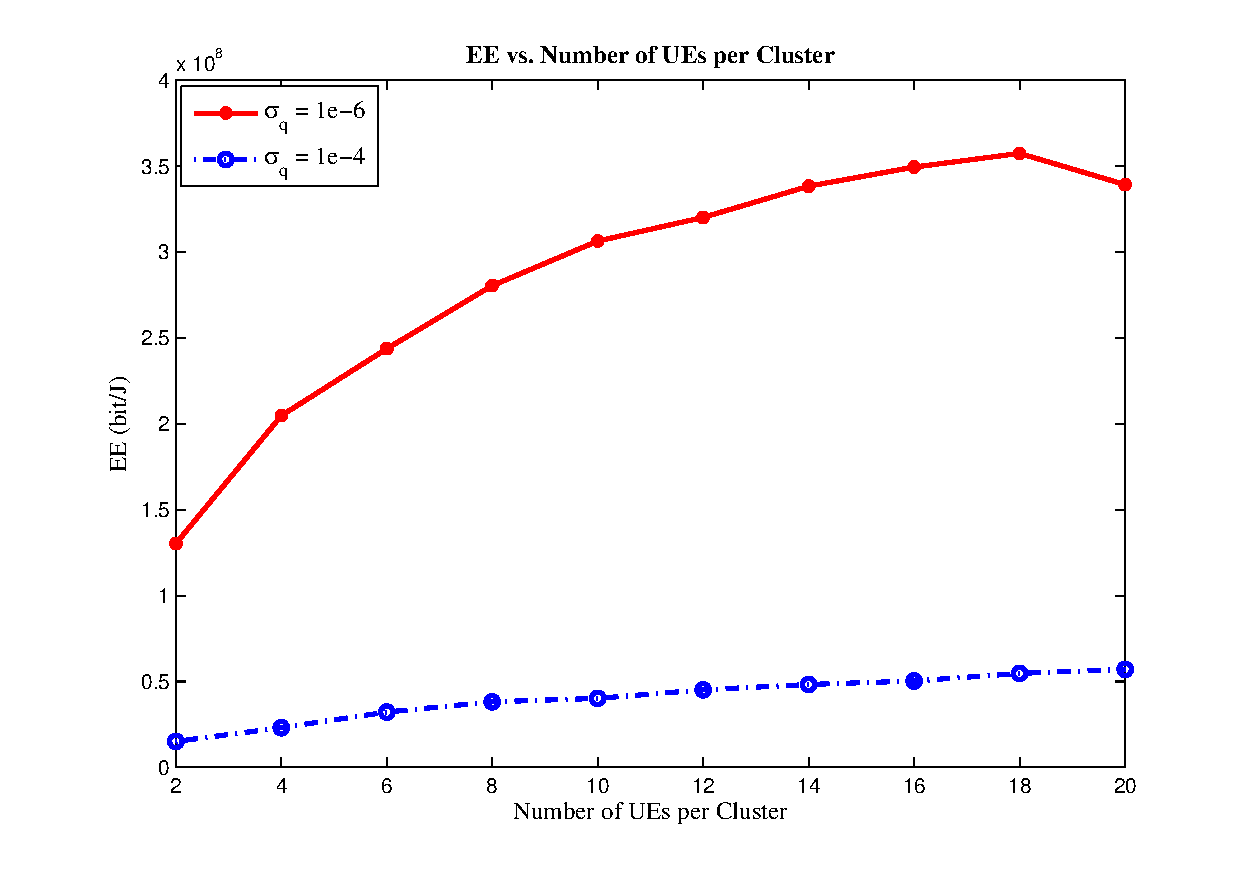
\includegraphics[width=\linewidth]{./fig3/varUE}
  \caption{  بازدهی انرژی بر حسب تعداد کاربران در 3 خوشه  برای دو مقدار 
  $\sigma_q = 1e-4 , 1e-6$
   100 واحد رادیویی
   در هر خوشه}
  \label{fig:Var}
\end{figure}
 حال در شکل \ref{fig:Var}، بازدهی انرژِی بر حسب تعداد کاربران در هر خوشه  برای برای دو مقدار 
  $\sigma_q = 10^{-4} , 10^{-6}$
   و وجود 3 خوشه در هر خوشه با فرض بودن  100 واحد رادیویی در هر خوشه رسم شده است.همانطور که می بینید با افزایش کاربران بازدهی انرژی افزایش یافته است و بازدهی انرژی در واریانس نویز کمتر بشتر از بازدهی انرژی در واریانس نویز بیشتر می باشد.
%    \begin{figure}[H]
%  \centering
%    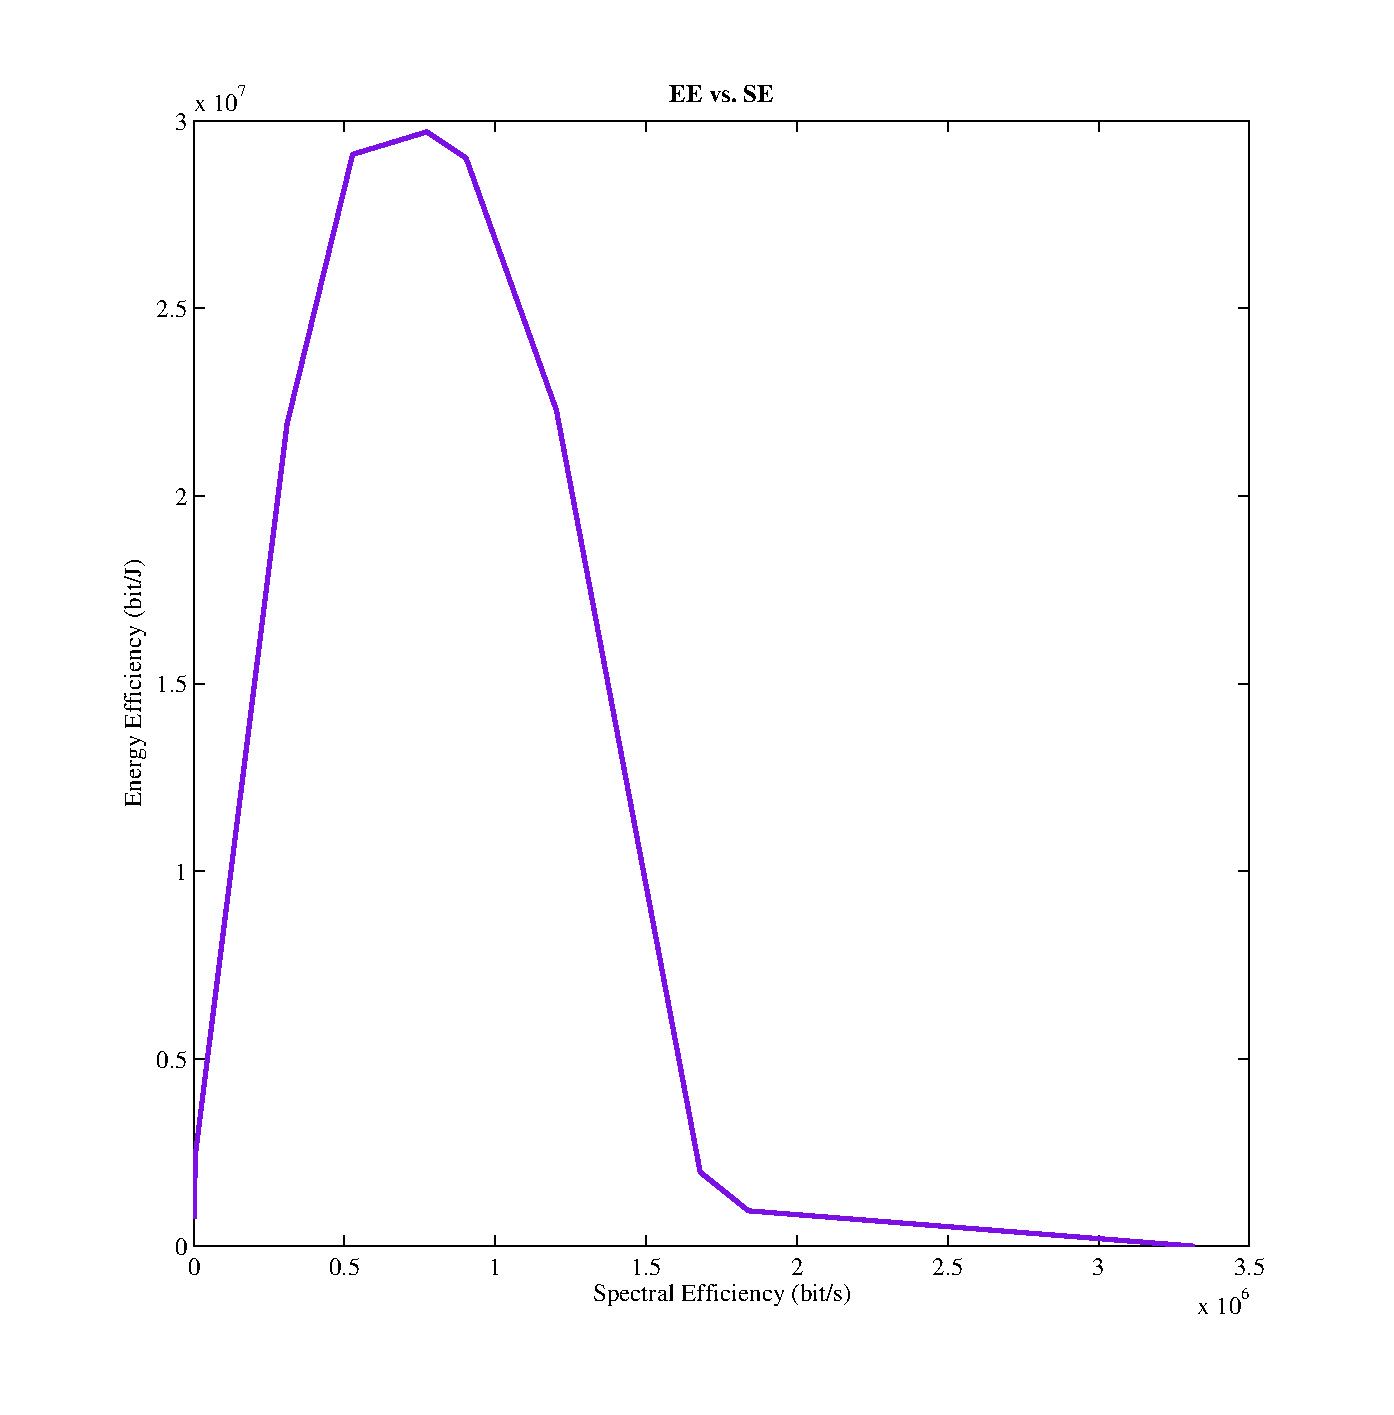
\includegraphics[width=\linewidth]{./fig3/spect}
%  \caption{  بازدهی انرژی بر حسب بازدهی طیف}
%  \label{fig:spect}
%\end{figure}
%در شکل \ref{fig:spect}، بازدهی انرژی بر حسب بازدهی طیف برای 2 خوشه که در هر خوشه 2 کاربر و 10 واحد رادیویی قرار دارد ($\sigma_q = 10^{-4}$)، رسم شده است. این نمودار با تغییر توان بیشینه ی هر واحد رادیویی رسم شده است. ابتدا با افزایش توان از مقدار 0 بازدهی انرژی بر حسب بازدهی طیف زیاد می شود و در نهایت با افزایش توان بازدهی انرژی بر حسب بازدهی طیف کاهش می یابد.  
\subsection{نتیجه گیری}
در این بخش، تخصیص توان بهینه در لینک فروسو برای مدل سیستم \lr{MIMO C-RAN} با فرض محدودیت بر روی ظرفیت \lr{fronthaul}، در نظر گرفته شده است. مدل سیستم شرح داده شده و مسئله ی تخصیص توان بهینه با روش الگوریتم بهینه و استفاده از تابع لاگرانژ حل شده است. شبیه سازی ها نشان می دهد که با افزایش تعداد واحدهای رادیویی عملکرد سیستم بهبود داده و افزایش تعداد کاربران ابتدا منجر به افزایش بازدهی انرژی می گردد و سپس به دلیل زیاد شدن تاثیر تداخل، \lr{EE} کاهش می یابد. همچنین با کاهش نویز کوانتیزاسیون عملکرد سیستم بهبود می یابد. علاوه بر این، با افزایش  بیشینه ظرفیت لینک \lr{fronthaul} ابتدا بازدهی انرژی زیاد شده سپس شیب افزایش بازدهی انرژی، کم می شود.
%%%%%%%%%%%%%%%%%%%%%%%%%%%%%%%%%%%%%%%%%%%%%%%%%
\section{لینک فراسو}
در این بخش، لینک فراسو برای سیستم \lr{MIMO C-RAN} در نظر گرفته شده است که  پیام در مسیر لینک فراسو از کاربر به واحدهای رادیویی منتقل می شود و پس از فشرده سازی توسط لینک \lr{fronthaul} به واحد کنترل منتقل می گردد. \newline
همانند لینک فروسو فرض بر این است که واحدهای رادیویی و کاربران خوشه بندی شده اند به طوری که هر خوشه  شامل تعدادی واحد رادیویی است که به کاربران موجود در آن خوشه، سرویس دهی می کنند.

 \begin{figure}
  \centering
    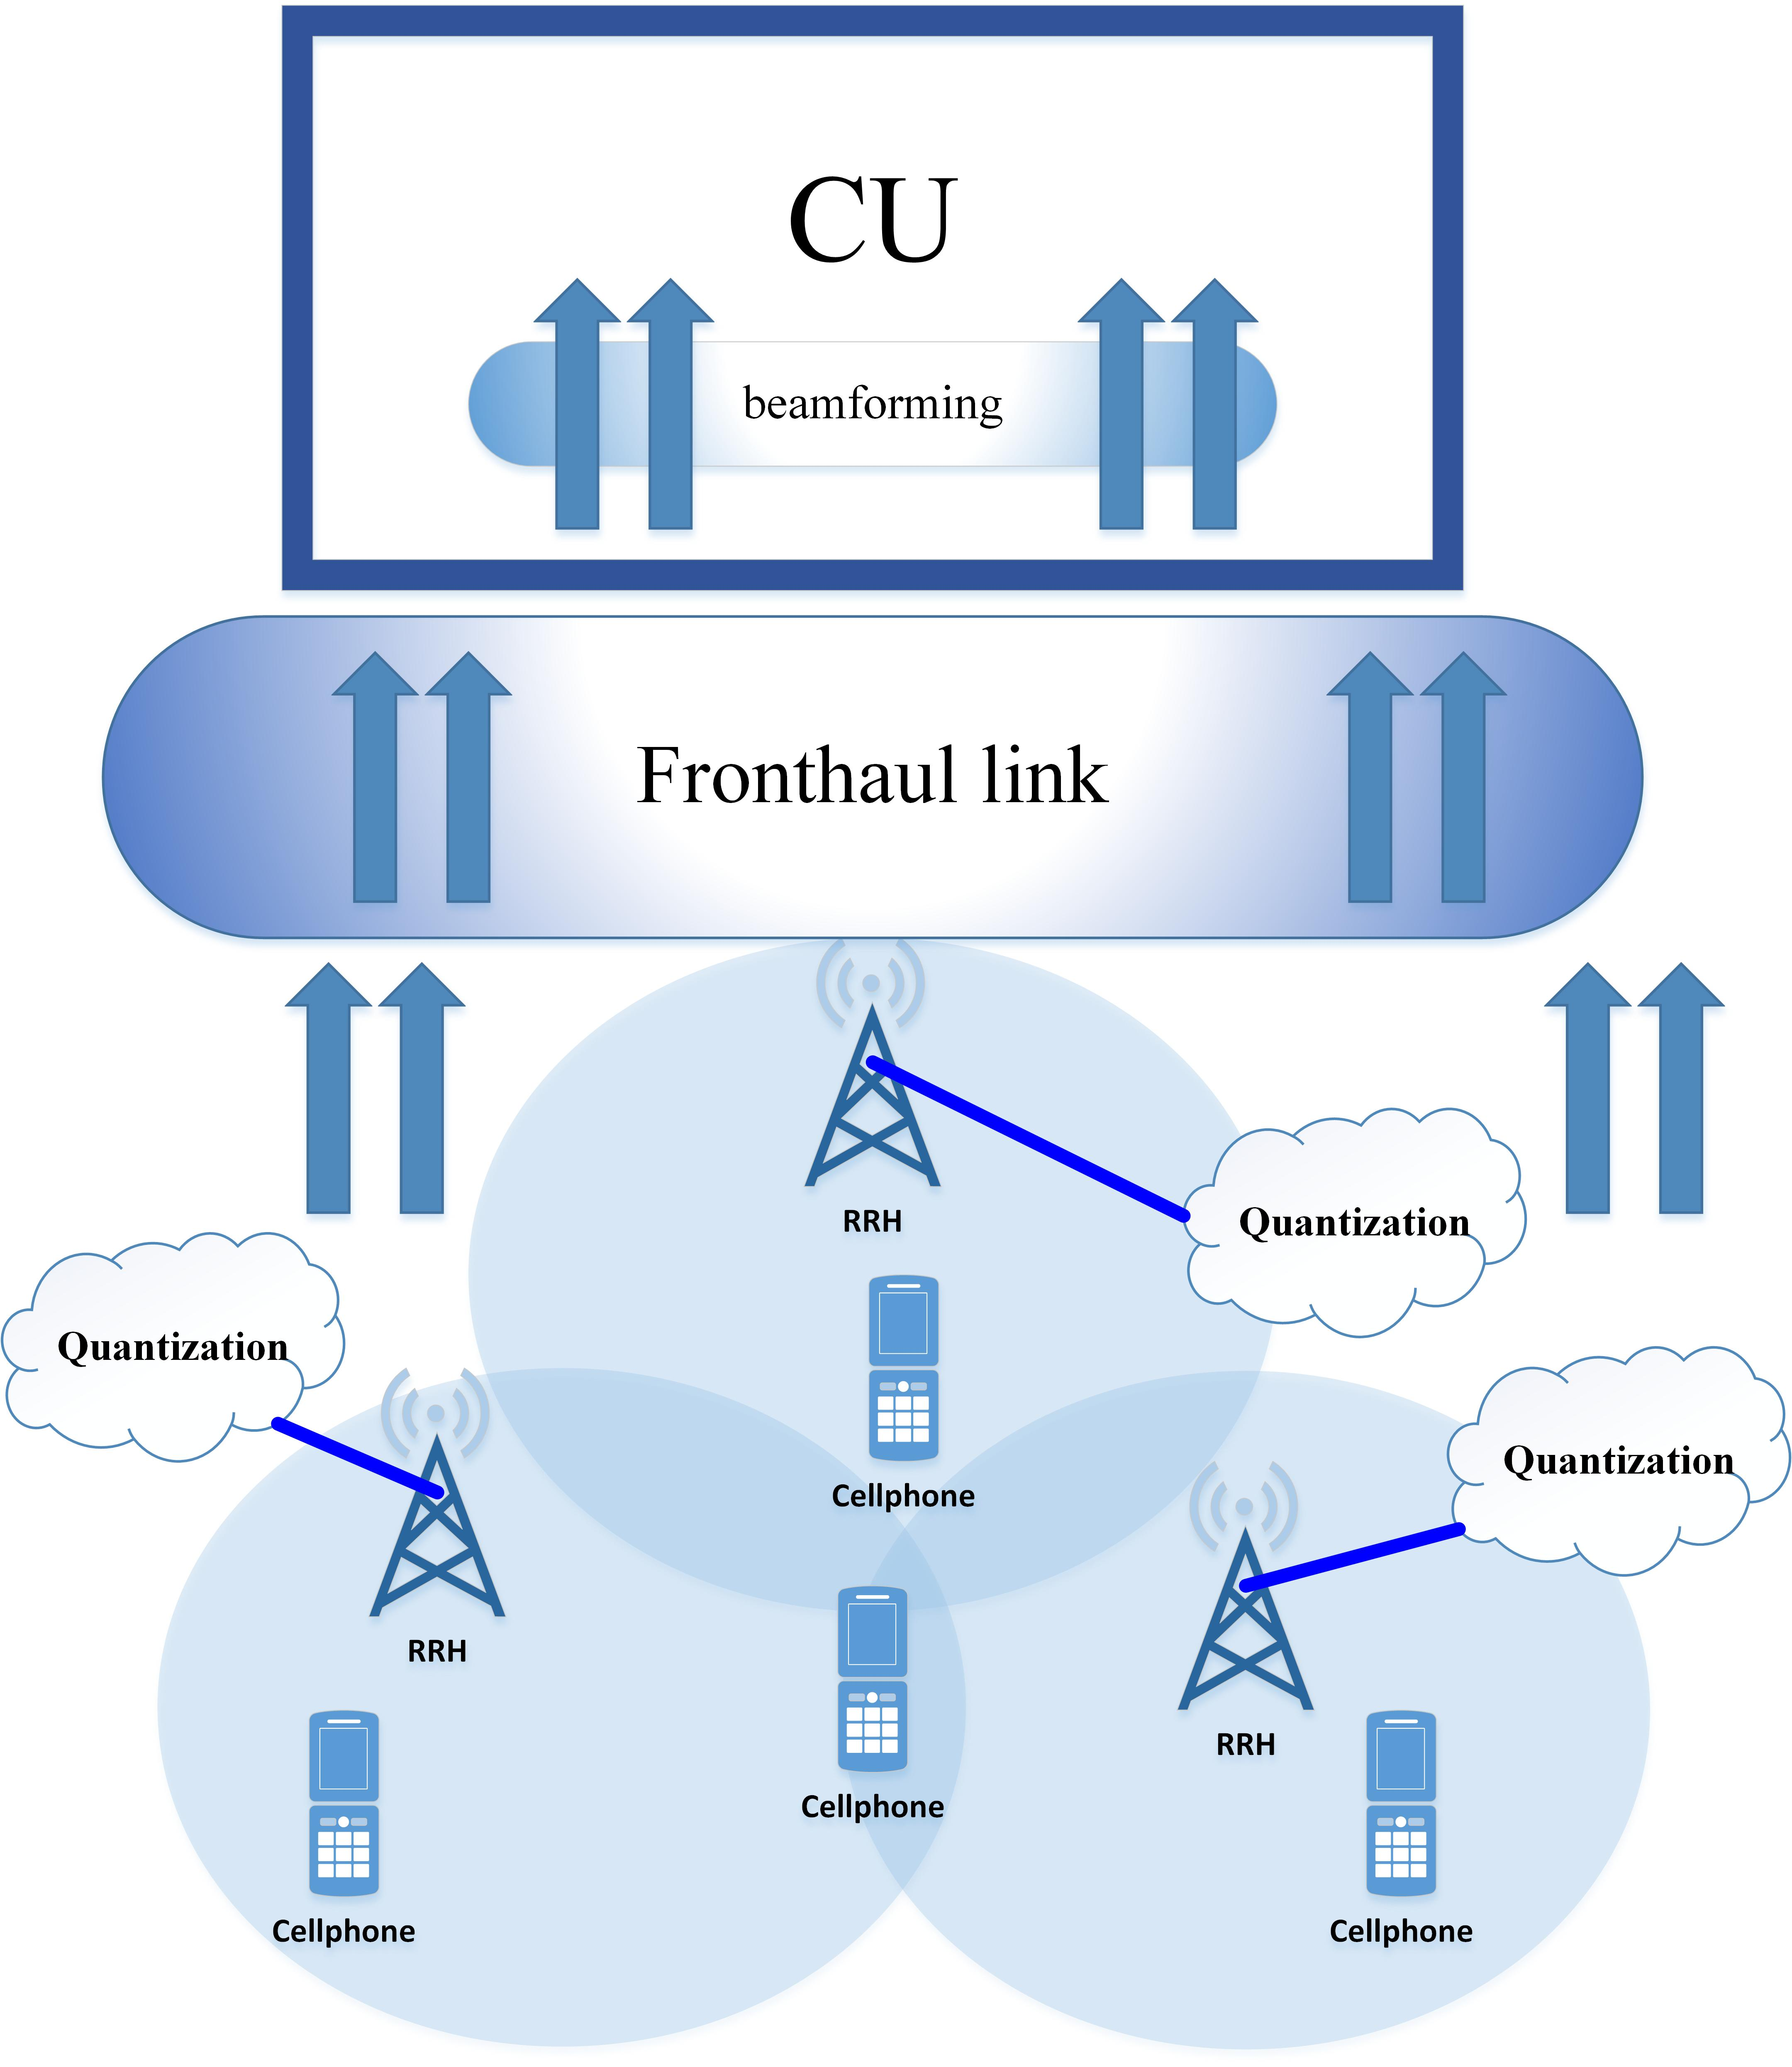
\includegraphics[scale = 0.45]{./fig/Drawing2}
  \caption{ساختار 
  \lr{C-RAN}
  در  لینک فراسو
  }
  \label{fig:cr2}
\end{figure}
همچنین در این مدل از روش پرتو دهی برای کاهش تداخل استفاده می کنیم که پرتو دهی در داخل واحد کنترل صورت می گیرد.
در ادامه، ابتدا سیستم  مدل و سپس نرخ قابل دسترسی بیان شده و مسئله ی تخصیص توان بررسی می گردد.
\subsection{مدل سیستم}
مدل سیستم برای لینک فراسو نیز همانند لینک فروسو می باشد که در ادامه شرح داده شده است\cite{ofdma,ulCompression}.
 سیستم \lr{MIMO C-RAN} شامل $R$ واحد رادیویی می باشد که $D$ کاربر تک آنتنه را سرویس می دهند.فرض بر این است که کاربران و واحد رادیوییها، به 
 $S$
خوشه تقسیم شده اند که $v$ امین خوشه،
 دارای $R_v$ واحد رادیویی است که ${D}_v$ کاربر را سرویس دهی می کنند.
 علاوه بر این، فرض بر این است که
$j$
امین واحد رادیویی، در $v$امین خوشه، توسط لینک فیبر نوری با ظرفیت محدود $c_{r_{(v,j)}}$ به واحد کنترل متصل می گردد.
\begin{equation}
\begin{split}
\mathcal{R}_v= \{  r_{(v,i)} | 1 \leq i \leq {R}_v , i\in Z^+\}, \\
\mathcal{C}_{\mathcal{R}_v}= \{C_{r_{(v,j)}}| 1 \leq j \leq {R}_v , j\in Z^+\}, \\
\mathcal{D}_v= \{  d_{(v,k)} | 1 \leq k \leq {D}_v , k\in Z^+\},  \\
\end{split}
\end{equation} 
که
 $\mathcal{R}_v$، $\mathcal{C}_{\mathcal{R}_v}$
 و
  $\mathcal{D}_v$
 به ترتیب نشان دهنده ی دسته واحد رادیوییها، دسته ی ظرفیت لینک \lr{Fronthaul} و دسته ی کاربران در $v$امین دسته ی خوشه می باشد.\newline
واحد رادیویی
ها تداخل پیام ها را از خوشه های دیگر نیز دریافت می کنند.\newline
 \subsection{آنالیز نرخ قابل دسترس}
در این قسمت، هدف بررسی نرخ قابل دسترسی سیستم می باشد.
\begin{theorem}\label{t1}
 نرخ قابل دسترسی برای کاربر $d_{(s,k)}$ به صورت زیر می باشد:
\begin{equation}\label{e1}
\mathfrak{R}_{d_{(s,k)}} = B \log_2(1+\gamma_{d_{(s,k)}}),
\end{equation}
که $B$ پهنای باند کانال و $\gamma_{d_{(s,k)}}$ همان \lr{SINR} دریافتی $k$امین کاربر در $s$امین دسته ی خوشه است که به صورت زیر بیان می گردد.  
\begin{equation}\label{5}
\gamma_{d_{(s,k)}}= \frac{p_{d_{(s,k)}} |{\boldsymbol{w}^H}_{\mathcal{R}_{s},d_{(s,k)}}^آ\boldsymbol{h}_{\mathcal{R}_s, d_{(s,k)}}|^2}{I_{d_{(s,k)}}+B\nu}.
\end{equation}
در فرمول \eqref{5}، 
$I_{d_{(s,k)}}$
نشان دهنده ی توان سیگنال تداخلی است.$B\nu$
نشان دهنده ی توان نویز است و
$\boldsymbol{h}_{\mathcal{R}_s, d_{(s,k)}}$ 
 نشان دهنده ی بردار کانال بین $k$امین کاربر و واحدهای رادیویی
 $s$
 امین دسته ی خوشه می باشد. همچنین 
 $\boldsymbol{w}_{\mathcal{R}_{s},d_{(s,k)}}$
 نشان دهنده ی بردار پرتو دهی استفاده شده در $s$امین دسته ی خوشه ها برروی واحدهای رادیویی برای بدست آوردن پیام $k$امین کاربر می باشد. 
 $p_{d_{(s,k)}}$
 توان ارسالی$k$امین کاربر در $s$امین دسته ی خوشه می باشد.
\end{theorem}
\begin{proof}
در این قسمت می خواهیم $\gamma$ را بدست آوریم

فرض کنید $\boldsymbol{y}_{\mathcal{R}_s}$ یک بردار
 $R_s \times 1$
باشد که نشان دهنده ی سیگنال دریافتی توسط دسته ای از واحدهای رادیویی در $s$
امین خوشه باشد که به صورت زیر بدست می آید.
\begin{equation} \label{1}
\boldsymbol{y}_{\mathcal{R}_s} = \sum_{v=1}^S \boldsymbol{H}_{\mathcal{R}_v,\mathcal{D}_s}{\boldsymbol{x}}_{\mathcal{D}_v}+ \boldsymbol{z}_{\mathcal{D}_s},
\end{equation}
که   ${\boldsymbol{x}}_{ \mathcal{D}_v} = [{x}_{ d_{(v,1)}},...,{ x}_{ d_{(v,\mathcal{D}_v)}}]^T \in \mathbb{C}^{{D}_v } $ 
بردار سمبل ارسالی خوشه ی  $v$ ام می باشد.\newline
 $\boldsymbol{z_{\mathcal{D}_s}} \backsim \mathcal{N}(0,N_0\boldsymbol{I}_{{D}_s})$ 
 نویز گوسی سفید اضافه شونده می باشد که دارای توان $N_0$
 و \newline
 $\boldsymbol{H}_{\mathcal{R}_v,\mathcal{D}_s}  \in \mathbb{C}^{{R}_v\times {D}_s}$ 
 نشان دهنده ی ماتریس کانال بین  کاربران $\mathcal{D}_s$ در دسته ی
 $s$
   ام و واحدهای رادیویی   $\mathcal{R}_v$ در دسته ی   $v$ ام می باشد.\newline
همچنین مدل کانال همانند لینک فروسو با توجه به فرمول \eqref{channel}، بدست می آید.
 حال می خواهیم پیام دریافتی توسط واحد رادیویی  $n$ ام در دسته ی $s$ ام را بدست آوریم:
 
\begin{equation} \label{100}
y_{r_{(s,n)}} = \sum_{k=1}^{D_s} h_{r_{(s,n)},d_{(s,k)}} \sqrt{p_{d_{(s,k)}}}  x_{d_{(s,k)}}
+\sum_{t=1,t\neq s}^{S} \sum_{j=1}^{D_t} h_{r_{(s,n)},d_{(t,j)}} \sqrt{p_{d_{(t,j)}}} x_{d_{(t,j)}}
 +z_{r_{(s,n)}}
\end{equation}
پیام دریافتی توسط واحد رادیویی، بعد از فشرده سازی به صورت زیر می شود
\begin{equation}
\hat{y}_{r_{(s,n)}} = y_{r_{(s,n)}} + q_{r_{(s,n)}} 
\end{equation}
پیام هر کاربر در واحد کنترل با اعمال پرتو دهی \LTRfootnote{beamforming} به صورتی که در ادامه بیان شده، بدست می آید

\begin{equation}
\begin{split}
\hat{x}_{d_{(s,k)}} = & {\boldsymbol{w}^H}_{\mathcal{R}_s, d_{(s,k)}} \boldsymbol{h}_{\mathcal{R}_s, d_{(s,k)}} \sqrt{p_{d_{(s,k)}}}  x_{d_{(s,k)}} \\
+ & \sum_{i=1,i\neq k}^{D_s}  {\boldsymbol{w}^H}_{\mathcal{R}_s, d_{(s,k)}} \boldsymbol{h}_{\mathcal{R}_s, d_{(s,i)}} \sqrt{p_{d_{(s,i)}}}  x_{d_{(s,i)}} \\
+&  \sum_{t=1,t\neq s}^{S} \sum_{j=1}^{D_t} {\boldsymbol{w}^H}_{\mathcal{R}_s, d_{(s,k)}} \boldsymbol{h}_{\mathcal{R}_s, d_{(t,j)}} \sqrt{p_{d_{(t,j)}}}  x_{d_{(t,j)}} \\
+& {\boldsymbol{w}^H}_{\mathcal{R}_s, d_{(s,k)}}  ({\boldsymbol{q}}_{\mathcal{R}_s} + {\boldsymbol{z}}_{\mathcal{R}_s})
\end{split}
\end{equation}
حال برای بدست آوردن  \lr{SINR}، توان سیگنال بر روی توان تداخل و نویز را بدست می آوریم:
\begin{equation}
\gamma = \frac{p_{d_{(s,k)}}|{\boldsymbol{w}^H}_{\mathcal{R}_s, d_{(s,k)}} \boldsymbol{h}_{\mathcal{R}_s, d_{(s,k)}}|^2}{
  I_{d_{(s,k)}}
+ B \times \nu_{d_{(s,k)}}
}
\end{equation}
که داریم :
\begin{equation}
\begin{split}
\nu_{d_{(s,k)}}&  = {\boldsymbol{w}^H}_{\mathcal{R}_s, d_{(s,k)}}  (diag({\sigma_n^2}_{r_{(s,1)}}...{\sigma_n^2}_{r_{(s,R_s)}})+diag({\sigma_q^2}_{r_{(s,1)}}...{\sigma_q^2}_{r_{(s,R_s)}})) {\boldsymbol{w}}_{\mathcal{R}_s, d_{(s,k)}}\\
I_{d_{(s,k)}}& = \sum_{i=1,i\neq k}^{D_s}  |{\boldsymbol{w}^H}_{\mathcal{R}_s, d_{(s,k)}} \boldsymbol{h}_{\mathcal{R}_s, d_{(s,i)}}|^2 p_{d_{(s,i)}} +\sum_{t=1,t\neq s}^{S} \sum_{j=1}^{D_t} |{\boldsymbol{w}^H}_{\mathcal{R}_s, d_{(s,k)}} \boldsymbol{h}_{\mathcal{R}_s, d_{(t,j)}}|^2 p_{d_{(t,j)}} 
\end{split}
\end{equation}
 در اینجا  $\sigma_n^2$ واریانس نویز می باشد که  برای سادگی برای همه ی واحدهای رادیویی ثابت فرض شده و  دارای مقدار $N_0$ 
است و $\sigma_q^2$ واریانس نویز فشرده سازی می باشد.
علاوه بر این با استفاده از پرتودهی \lr{MMSE}، ماتریس پرتودهی به صورت زیر است 
\begin{equation}
\boldsymbol{W}_{\mathcal{R}_s,\mathcal{D}_s} = \hat{\boldsymbol{H}}_{\mathcal{R}_s,\mathcal{D}_s}(\hat{\boldsymbol{H}}_{\mathcal{R}_s,\mathcal{D}_s}^H \hat{\boldsymbol{H}}_{\mathcal{R}_s,\mathcal{D}_s}+ \alpha \boldsymbol{I}_{{D}_s})^{-1},
\end{equation} 
همچنین  $\alpha$، فاکتور رگولاریزاسیون است در صورتی که $\alpha$ صفر یاشد، ماتریس پرتو دهی \lr{ZF} خواهیم داشت.
\end{proof}
\subsection{بهینه سازی تخصیص توان}
در این قسمت می خواهیم توان را طوری اختصاص دهیم تا بازدهی انرژی به بیشینه مقدار خود برسد.
می دانیم نرخ قابل دسترس بر روی لینک \lr{fronthaul}، بین $n$ امین واحد رادیویی در $s$ امین خوشه  و  واحد کنترل به صورت زیر بدست می آید 
\begin{equation}
C_{r_{(s,n)}} = \log{\frac{1+( \sum_{k=1}^{D_s}|h_{r_{(s,n)},d_{(s,k)}}|^2{p_{d_{(s,k)}}} + \sum_{t=1,t\neq s}^{S}\sum_{l=1}^{D_t}|h_{r_{(s,n)},d_{(t,l)}}|^2{p_{d_{(t,l)}}}+ B N_0) }{ \sigma_{q_{(s,n)}}^2})},
\end{equation}
\subsubsection{شرح مسئله}
 همانطور که گفته شد نسبت مجموع نرخ ها در سیستم به کل توان ارسالی کاربرها نشان دهنده ی بازدهی انرژی است که با $\eta$ نمایش داده می شود و می توان اینگونه بیان کرد
\begin{equation}\label{eta1}
\eta(\boldsymbol{P}) := \frac{\sum\limits_{s=1}^{S} \sum\limits_{k=1}^{{D}_s}\mathfrak{R}_{d_{(s,k)}} }{\sum\limits_{s=1}^{S} \sum\limits_{k=1}^{{K}_s}{p}_{d_{(s,k)}}} = \frac{R_{total}(\boldsymbol{P})}{P_{UE}(\boldsymbol{P})},
\end{equation}
که در اینجا  $ \boldsymbol{P} = \{ \boldsymbol{P}_{\mathcal{D}_s}|  1 \leq s \leq S, s \in \mathbb{Z}^{+} \}$ ماتریس تخصیص توان است. در این بخش، بیشینه سازی بازدهی انرژی با شروط زیر مورد بررسی قرار می گیرد 
\begin{equation}\label{p11}
\begin{aligned}
\max\limits_{\boldsymbol{P}}   \quad &   \eta(\boldsymbol{P})\\
\text{\lr{subject to}} \quad  &  0 \leq {p}_{d_{(s,k)}} \leq P_{max} && \qquad \forall s, \forall k,   \\
&\mathfrak{R}_{d_{(s,k)}} \geq  \mathfrak{R}_{d_{(s,k)}}^{th} && \qquad \forall s, \forall k, \\ 
&C_{r_{(s,i)}} \leq C_{r_{(s,i)}}^{th}  &&\qquad \forall s, \forall i, \\
\end{aligned}			
\end{equation}
همانند لینک فروسو، بدلیل محدب نبودن مسئله از روش الگوریتم تکرار شونده استفاده می کنیم.
\subsection{روش مورد استفاده}
در این قسمت، به جای ماکسیمم کردن \eqref{eta1}، همانند لینک فروسو، از قضیه ی \eqref{t2} استفاده می نماییم.
 همچنین کران بالایی برای تداخل بدست می آید که در ادامه بیان می شود.
\begin{equation} \label{id}
\tilde{I}_{d_{(s,k)}} = \sum_{v=1}^{S}  |{\boldsymbol{w}^H}_{\mathcal{R}_s, d_{(s,k)}} \boldsymbol{h}_{\mathcal{R}_v, d_{(s,i)}}|^2 P_{max} 
\end{equation}
در نتیجه با توجه به رابطه ی  \eqref{id}، می توان $\gamma$ را به این صورت تخمین زد:
\begin{equation}
\tilde{\gamma}_{d_{(s,k)}}= \frac{p_{d_{(s,k)}} |{\boldsymbol{w}^H}_{\mathcal{R}_{s},d_{(s,k)}}^آ\boldsymbol{h}_{\mathcal{R}_s, d_{(s,k)}}|^2}{\tilde{I}_{d_{(s,k)}}+B\nu}.
\end{equation}
ابتدا تابع لاگرانژ را تشکیل می دهیم تا بتوان با استفاده از آن، از الگوریتم تکرار شونده ی \eqref{alg}، استفاده کرد. 
\begin{equation}
\begin{split}
\mathcal{L}(\boldsymbol{P}; \boldsymbol{\lambda}, \boldsymbol{\mu}, \boldsymbol{ \kappa}) & = \sum\limits_{s=1}^{S} \sum\limits_{k=1}^{\mathcal{D}_s}\mathfrak{\tilde{R}}_{d_{(s,k)}} 
- \eta \sum\limits_{s=1}^{S} \sum\limits_{k=1}^{\mathcal{K}_s}{p}_{d_{(s,k)}}\\
&+\sum\limits_{s=1}^{S} \sum\limits_{k=1}^{\mathcal{D}_s} \lambda_{d_{(s,k)}} (\mathfrak{\tilde{R}}_{d_{(s,k)}}-\mathfrak{R}_{d_{(s,k)}}^{th})\\
&- \sum\limits_{s=1}^{S} \sum\limits_{k=1}^{\mathcal{K}_s} \mu_{d_{(s,k)}} ({p}_{d_{(s,k)}}-P_{max})\\
&- \sum\limits_{s=1}^{S} \sum\limits_{i=1}^{\mathcal{R}_s} \kappa_{r_{(s,i)}} (C_{r_{(s,i)}}-C_{r_{(s,i)}}^{th}).\\
\end{split}
\end{equation}
که در اینجا، $\boldsymbol{\lambda}, \boldsymbol{\mu}, \boldsymbol{\kappa} \geq 0$
بردارهای ضرایب لاگرانژ می باشد .\newline
با استفاده از این معادله و مشتقگیری از آن، توان بهینه به صورت زیر بدست می آید
\begin{equation}
p_{d_{(s,k)}}^* \approx [\frac{ B(1+\lambda_{d_{(s,k)}} )-(\sum_{n=1}^{\mathcal{R}_s}\kappa_{r_{(s,i)}})}{\ln2 \times (\eta + \mu_{d_{(s,k)}})}]^+;
\end{equation} 

  در آخر، برای بدست آوردن توان بهینه، الگوریتم \eqref{alg1} مورد استفاده قرار می گیرد \cite{hcranEE}
 \begin{latin}
\begin{algorithm}
\caption{Energy-Efficient Power Allocation}\label{alg1}
\begin{algorithmic}

\State Set the maximum number of iterations $I_{max}$, convergence condition $\epsilon_{\eta}$  and the initial value $\eta^{(1)} = 0$
\State Set the iteration index $i = 1$ and begin the iteration (Outer
Loop).
\For {$ 1\leq i \leq  Imax$}
\State Solve the resource allocation problem with $\eta^{(i)}$ (Inner Loop);
\State Obtain $P^{(i)}, R_{total}^{(i)}, P_{UE}^{(i)}$
\If {$ R_{total}(\boldsymbol{P}^{(i)}) - \eta^{(i)} P_{UE}(\boldsymbol{P}^{(i)}) < \epsilon_{\eta} $} 
\State Set $\boldsymbol{P}^*= \boldsymbol{P}^{(i)} $   and  $ \eta^{*} =\eta^{(i)} $;
\State break;
\Else
\State Set $\eta^{(i)}= \frac{R_{total}(\boldsymbol{P}^{(i))}}{P_{UE}(\boldsymbol{P}^{(i))}}$ and $i= i+1$;
\EndIf 
\State \textbf{end if}
\EndFor 
\State \textbf{end for}

\end{algorithmic}
\end{algorithm}
\end{latin}
\subsection{نتایج عددی}
در این بخش، نتایج عددی الگوریتم مورد استفاده را برای سیستم \lr{MIMO C-RAN} با پارامترهای بیان شده در جدول \ref{tab:title3} و استفاده از پرتو دهی \lr{ZF} بیان می شود.
\begin{latin} 
 \begin{table}[H]
 \caption {\rl{پارامترهای شبیه سازی}} \label{tab:title3} 
 \begin{center}
  \begin{tabular}{||c c ||} 
  \hline
  Parameter & Value \\ [0.5ex] 
  \hline\hline
  Number of cluster S & 3 \\ 
  \hline
  Noise power density & -174dBm/Hz\\
  \hline
  Bandwidth & 120KHz \\
  \hline
 Maxmimun transmit Power & 10dBm \\
  \hline
  Circuit Power of whole RRHs & 10dBm \\
  \hline
  Variance of quantization noise & $10^{-2}$ \\
  \hline
   Maxmimun fronthaul link's rate & 20bits/sec/Hz \\
  \hline
  Minimum data rate &  1bits/sec/Hz \\ [1ex] 
  \hline
 \end{tabular}
 \end{center}
 \end{table}
 \end{latin}
  \begin{figure}[H]
  \centering
    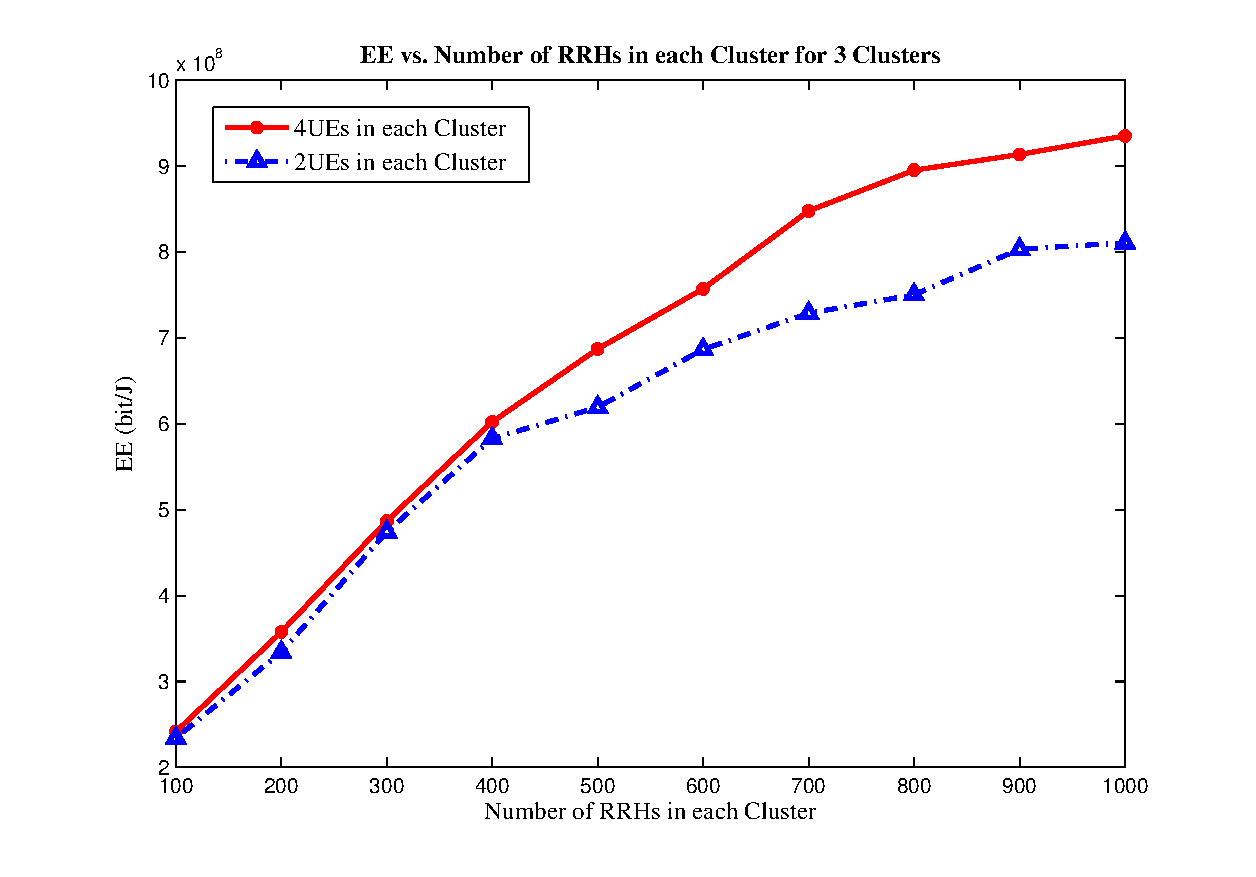
\includegraphics[width=\linewidth, height=12cm]{./fig3/rrhul}
  \caption{
  بازدهی انرژی با توجه به تغییرات تعداد واحدهای رادیویی  در هر خوشه برای توان بهینه  برای 
   دو کاربر مختلف
   و پارامترهای جدول \ref{tab:title3}}
  \label{fig:rrhul}
\end{figure}
 در شکل \ref{fig:rrhul}، بازدهی انرژی سیستم \lr{MIMO C-RAN} بر اساس تعداد واحدهای رادیویی در هر خوشه برای الگوریتم مورد استفاده و برای دو تعداد کاربر متفاوت، رسم شده است. 
 همانطور که  شکل  نشان می دهد، با افزایش تعداد واحدهای رادیوی، بازدهی انرژی افزایش می یابد و از یک مقدار به بعد شیب افزایش بازدهی انرژی کمتر شده است. زیرا با افزایش تعداد واحدهای رادیویی، مجموع توان کل افزایش یافته و در نتیجه نرخ انتقال داده نیز بیشتر می گردد.

 \begin{figure}[H]
  \centering
    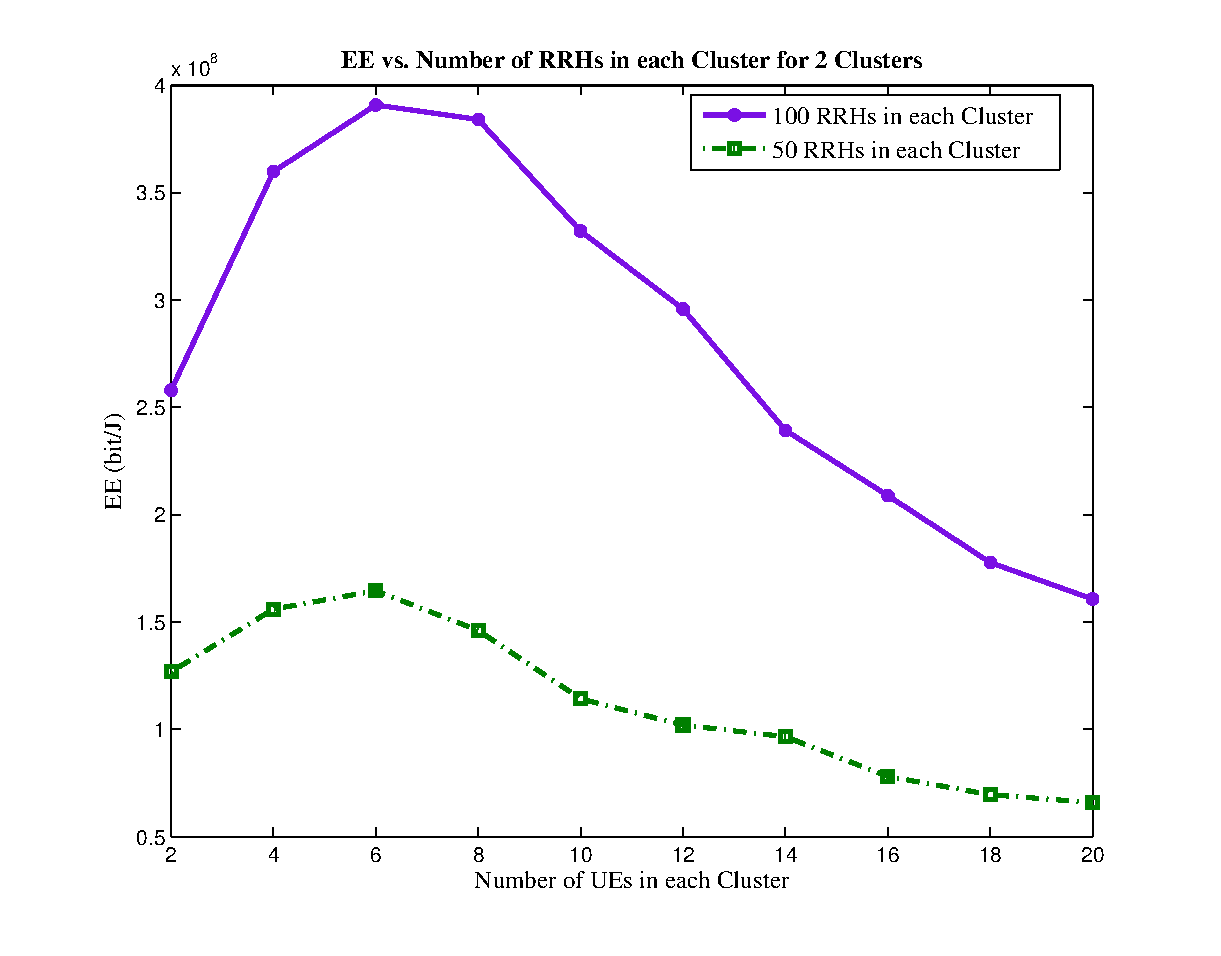
\includegraphics[width=\linewidth]{./fig3/ueul}
  \caption{  بازدهی انرژی با توجه به تغییرات تعداد کاربران در هر خوشه برای توان بهینه برای 
   دو واحد رادیویی مختلف
   و پارامترهای جدول \ref{tab:title3} و $S=2$}
  \label{fig:ueul}
\end{figure}


در شکل \ref{fig:ueul}، بازدهی انرژی بر اساس تعداد کاربران در هر خوشه برای الگوریتم مورد استفاده و برای دو تعداد واحد رادیویی متفاوت، رسم شده است. همانطور که  دیده می شود با افزایش تعداد کاربران، ابتدا شیب نمودار زیاد می شود و بازدهی انرژی افزایش می یابد سپس به دلیل افزایش تاثیر تداخل بین کاربران بازدهی انرژی کاهش می یابد. 

\begin{figure}[H]
  \centering
    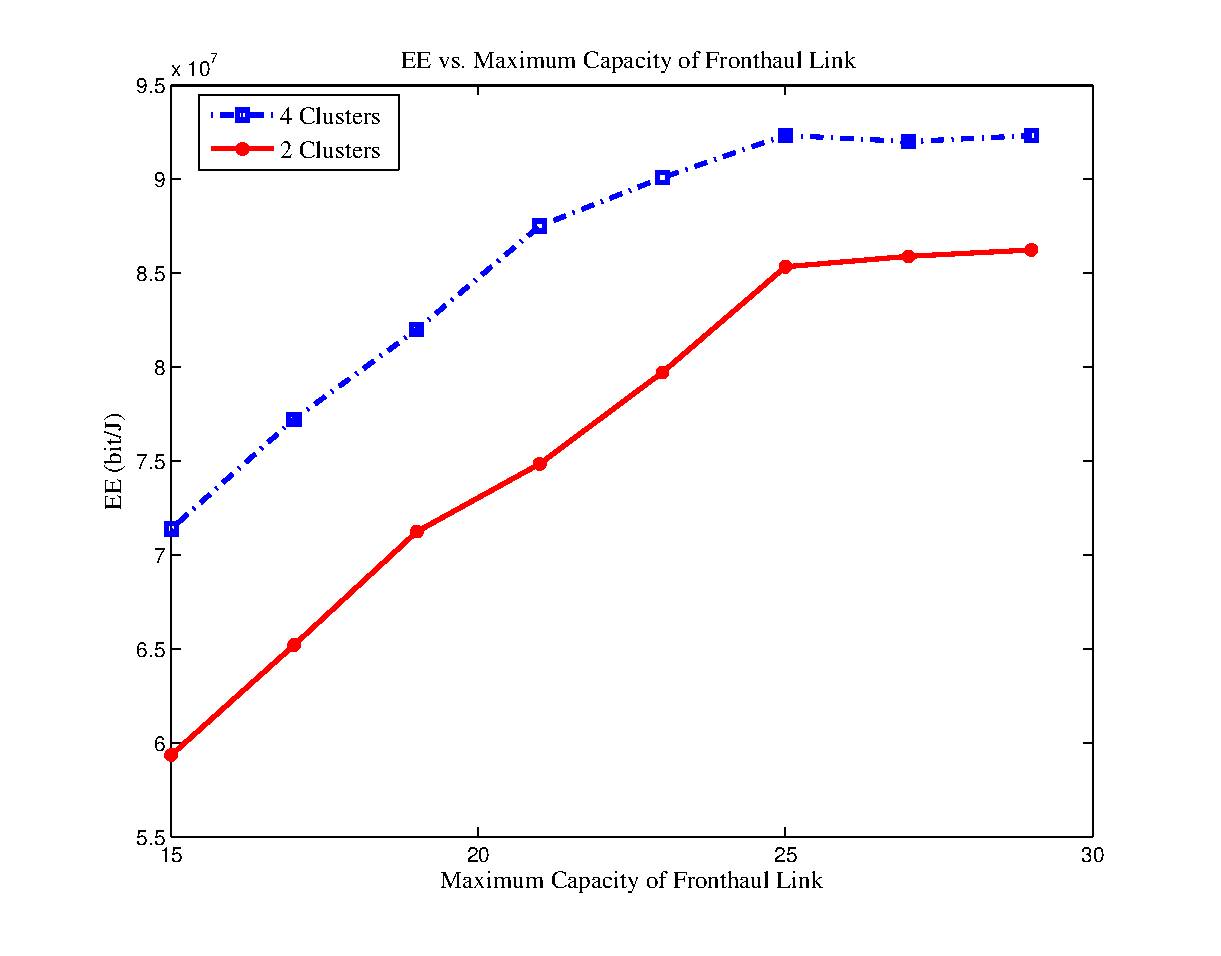
\includegraphics[width=\linewidth]{./fig3/cap}
  \caption{  بازدهی انرژی با توجه به تغییرات $C^{th}$، در در حالت $S =2 ,4 $, $\text{\lr{Number of RRHs per Cluster}} = 30$, $\text{\lr{Number of UE per Cluster}} =2$ }
  \label{fig:cap}
\end{figure}

در شکل \ref{fig:cap}، بازدهی انرژی بر اساس محدودیت ظرفیت لینک \lr{fronthaul}، برای دو تعداد متفاوت  2 و 4 خوشه و در هر خوشه 2 کاربر و 30 واحد رادیویی رسم شده است. با توجه به شکل، ابتدا با بازدهی انرژی، افزایش یافته،
سپس بدلیل اینکه نرخ قابل دسترس توسط تعداد کاربران و واحدهای رادیویی محدود می گردد، به نظر می آید افزایش محدودیت این ظرفیت تاثیر چندانی در بازدهی انرژی ندارد.  
\subsection{نتیجه گیری}
در این بخش، تخصیص توان بهینه در لینک فراسو برای مدل سیستم \lr{MIMO C-RAN} با فرض محدودیت بر روی ظرفیت \lr{fronthaul} و وجود چندین خوشه، در نظر گرفته شده است. مدل سیستم  شرح داده شده و مسئله ی تخصیص توان بهینه با روش الگوریتم بهینه و استفاده از تابع لاگرانژ حل شده است. شبیه سازی ها نشان می دهد همانند لینک فروسو با افزایش تعداد واحدهای رادیویی عملکرد سیستم بهبود داده و افزایش تعداد کاربران منجر به افزایش بازدهی انرژی می گردد ولی در نهایت به دلیل تداخل بازدهی انرژی کاهش می یابد. همچنین، با افزایش  بیشینه ظرفیت لینک \lr{fronthaul} ابتدا بازدهی انرژی زیاد شده سپس شیب افزایش بازدهی انرژی، کم می شود.
%%%%%%%%%%%%%%%%%%%%%%%%%%%%%%%%%%%%%%%%%%%%%%
\chapter{تخصیص منابع در حالت تقسیم زمانی دینامیکی در شبکه دسترسی رادیویی}
\section{مقدمه}
در این فصل هدف بدست آوردن مدل سیستم در حالت تقسیم زمانی یا \lr{TDD} \LTRfootnote{Time Division Duplexing} دینامیکی می باشد که بدین منظور تخصیص توان برای هر دو لینک فراسو و فروسو به طور همزمان بدست می آید.
در تقسیم زمانی دینامیکی، منابع به صورت دینامیکی بین هر دو لینک فراسو و فروسو  تخصیص داده می شود. در سیستم های سنتی  ایستگاه پایه و سیستم سنتی ایستگاه پایه و واحد رادیویی که در فصل اول بیان شد، تداخل بین لینک فراسو و فروسو منجر به کاهش شدید در بازدهی انرژی می گردد در حالی که در سیستم \lr{C-RAN} این تداخل  به دلیل وجود \lr{BBU Pool} و واحد های رادیویی \lr{RRH} و نوع پردازش هایی که در آنها صورت می گیرد، تاثیر چندانی در بازدهی انرژی نمی گذارد \cite{TDD,dynamic}.


حال در ادامه، مدل سیستمی با ساختار \lr{C-RAN}  بیان می نماییم که دارای چندین خوشه است که تعدادی از این خوشه  ها در لینک فراسو و تعدادی دیگر در لینک فروسو عمل می کنند. همچنین تمام واحدهای رادیویی در این خوشه ها به واحد کنترل ابری \lr{BBU Pool} از طریق لینک \lr{fronthaul} با ظرفیت محدود، متصلند. سیگنالهای خوشه های لینک فراسو و فروسو نیز بر یکدیگر تداخل اعمال می کنند.
\section{مدل سیستم}
در این بخش مدل سیستمی برای حالت تقسیم زمانی دینامیکی  براساس معماری \lr{C-RAN} در لینک فراسو و فروسو همانند فصل 3 بیان می شود. فرض بر این است که این سیستم شامل $S$ خوشه می باشد که $S_1$ خوشه در لینک فروسو و $S_2$
 خوشه در لینک فراسو عمل می کنند که :
 $S_1 + S_2 = S$
 است.
 همچنین هر خوشه ی $v$ دارای  $R_v$  واحد رادیویی و $D_v$ کاربر می باشد.  
 علاوه براین، فرض بر این است که
$j$
امین واحد رادیویی، در $v$امین خوشه، توسط لینک فیبر نوری با ظرفیت محدود $C_{r_{(v,j)}}$ به واحد کنترل متصل می گردد. در نتیجه داریم:
\begin{equation}
\begin{split}
\mathcal{R}_v= \{  r_{(v,i)} | 1 \leq i \leq {R}_v , i\in Z^+\}, \\
\mathcal{C}_{\mathcal{R}_v}= \{C_{r_{(v,j)}}| 1 \leq j \leq {R}_v , j\in Z^+\}, \\
\mathcal{D}_v= \{  d_{(v,k)} | 1 \leq k \leq {D}_v , k\in Z^+\},  \\
\end{split}
\end{equation} 
که
 $\mathcal{R}_v$، $\mathcal{C}_{\mathcal{R}_v}$
 و
  $\mathcal{D}_v$
 به ترتیب نشان دهنده ی دسته واحدهای رادیویی، دسته ی ظرفیت لینک \lr{Fronthaul} و دسته ی کاربران در $v$امین دسته ی خوشه می باشد.\newline
واحدهای رادیویی
 تداخل پیام ها را از خوشه های دیگر لینک فراسو و فروسو دریافت می کنند.
\newline
 \subsection{آنالیز نرخ قابل دسترس در خوشه های فروسو}
در این قسمت، هدف بررسی نرخ قابل دسترسی سیستم برای خوشه هایی است که در حال تبادل در لینک فروسو می باشند.
 نرخ قابل دسترسی برای کاربر $d_{(s,k)}$ به صورت زیر می باشد:
\begin{equation}\label{e1}
\mathfrak{R}_{d_{(s,k)}} = B \log_2(1+\gamma_{d_{(s,k)}}),
\end{equation}
که $B$ پهنای باند کانال و $\gamma_{d_{(s,k)}}$ همان \lr{SINR} دریافتی $k$امین کاربر در $s$امین دسته ی خوشه است که به صورت زیر بیان می گردد.  
\begin{equation}\label{51}
\gamma_{d_{(s,k)}}= \frac{p_{d_{(s,k)}}|\boldsymbol{h}_{\mathcal{R}_s, d_{(s,k)}}^H \boldsymbol{w}_{\mathcal{R}_{s},d_{(s,k)}}|^2}{I_{d_{(s,k)}}+BN_0}.
\end{equation}
در فرمول \eqref{51}، 
$I_{d_{(s,k)}}$
نشان دهنده ی توان سیگنال تداخلی است.$BN_0$
نشان دهنده ی توان نویز است و
$\boldsymbol{h}_{\mathcal{R}_s, d_{(s,k)}}$ 
 نشان دهنده ی بردار گین کانال بین $k$امین کاربر و واحدهای رادیویی
 $s$
 امین دسته ی خوشه در حالت لینک فروسو می باشد. همچنین 
 $\boldsymbol{w}_{\mathcal{R}_{s},d_{(s,k)}}$
 نشان دهنده ی بردار پیش کدگذاری استفاده شده در $s$امین دسته ی خوشه ها برای $k$امین کاربر می باشد. 
 $p_{d_{(s,k)}}$
 توان ارسالی واحدهای رادیویی است که به $k$امین کاربر در $s$امین دسته ی خوشه ارسال می گردد.


برای بدست آوردن  $\gamma_{d_{(s,k)}}$، ابتدا سیگنال دریافتی را نمایش می دهیم. سیگنال دریافتی لینک فروسو توسط کاربر $k$ ام در خوشه ی $s$ ام به این صورت نمایش داده می شود
\begin{equation}\label{6}
\begin{split}
y_{d_{(s,k)}} &= \underbrace{\sqrt{p_{d_{(s,k)}}}\boldsymbol{h}_{\mathcal{R}_s, d_{(s,k)}}^H \boldsymbol{w}_{\mathcal{R}_{s},d_{(s,k)}} x_{d_{(s,k)}} }_{\text{\lr{(desired signal)}}} + \underbrace{\sum_{\substack{l=1 \\ l\neq k}}^{{D}_s} \boldsymbol{h}_{\mathcal{R}_s, d_{(s,k)}}^H \boldsymbol{w}_{\mathcal{R}_{s},d_{(s,l)}}  \sqrt{p_{d_{(s,l)}}}  x_{d_{(s,l)}}}_{\text{(\lr{intra-cluster interference})}}\\
&+\underbrace{\sum_{\substack{v=1 \\ v\neq s}}^{S_1} \sum_{l=1}^{{D}_v} \boldsymbol{h}_{\mathcal{R}_v, d_{(s,k)}}^H \boldsymbol{w}_{\mathcal{R}_{v},d_{(v,l)}} 
\sqrt{p_{d_{(v,l)}}}  x_{d_{(v,l)}}}_{\text{(\lr{inter-cluster interference})}}+\underbrace{\sum_{\substack{t=1}}^{S_2} \sum_{l=1}^{{D}_t} \boldsymbol{b}_{\mathcal{D}_t, d_{(s,k)}}^H \sqrt{ p_{d_{(t,l)}}}  x_{d_{(t,l)}}}_{\text{(\lr{ interference from uplink's clusters})}}  \\
& +\underbrace{ \sum_{v=1}^{S_1} \sum_{i=1}^{{R}_v} q_{r_{(v,i)}} h_{r_{(v,i)}, d_{(s,k)}} }_{\text{(\lr{quantization noise interference})}}+ z_{d_{(s,k)}} .\\
\end{split}
\end{equation}
که در اینجا،
 $\boldsymbol{b}_{\mathcal{D}_t, d_{(s,k)}}  \in \mathbb{C}^{\mathcal{D}_t\times 1}$
 ، بردار کانال بین کاربران لینک فراسو در خوشه ی $t$ ام به $k$امین کاربر لینک فروسو در خوشه ی   $s$
 ام 
می باشد که همانند پارامتر بردار کانال $h$ بدست می آید. بقیه ی پارامترها نیز در فصل 3 به طور کامل بیان شده است.\\
با توجه به \eqref{6}، 
$I_{d_{(s,k)}}$ 
از رابطه ی زیر  بدست می آید.
\begin{equation}\label{7}
\begin{split}
I_{d_{(s,k)}} &=  \underbrace{\sum_{\substack{l=1 \\ l\neq k}}^{{D}_s} |\boldsymbol{h}_{\mathcal{R}_s, d_{(s,k)}}^H \boldsymbol{w}_{\mathcal{R}_{s},d_{(s,l)}}|^2  p_{d_{(s,l)}}}_{\text{(\lr{intra-cluster interference})}}
+\underbrace{\sum_{\substack{v=1 \\ v\neq s}}^{S_1} \sum_{l=1}^{{D}_v} |\boldsymbol{h}_{\mathcal{R}_v, d_{(s,k)}}^H \boldsymbol{w}_{\mathcal{R}_{v},d_{(v,l)}}|^2 p_{d_{(v,l)}}}_{\text{(\lr{inter-cluster interference})}}\\
&+\underbrace{\sum_{\substack{t=1}}^{S_2} \sum_{l=1}^{{D}_t} |\boldsymbol{b}_{\mathcal{D}_t, d_{(s,k)}}^H|^2  p_{d_{(t,l)}}}_{\text{(\lr{ interference from uplink's clusters})}} 
 +\underbrace{ \sum_{v=1}^{S_1} \sum_{i=1}^{{R}_v} {\sigma_q}_{r_{(v,i)}}^2  |h_{r_{(v,i)}, d_{(s,k)}}|^2 }_{\text{(\lr{quantization noise interference})}}.
\end{split}
\end{equation}
  همچنین توان سیگنال ارسالی به این صورت بدست می آید
\begin{equation}
\bar{p}_{r_{(s,i)}} = \boldsymbol{w}_{r_{(s,i)},\mathcal{D}_{s}} \boldsymbol{P}_{\mathcal{D}_s}^{\frac{1}{2}} \boldsymbol{P}_{\mathcal{D}_s}^{H \frac{1}{2}}   \boldsymbol{w}_{r_{(s,i)},\mathcal{D}_{s}}^H + \sigma_{q_{(s,i)}}^2 .
\end{equation}
و داریم:
\begin{equation}
P_{dl}= \sum_{s=1}^{S_1}\sum_{i=1}^{R_s}\bar{p}_{r_{(s,i)}} + P_c^{total,DL}
\end{equation}
که $ P_c^{total,DL}$، توان مداری کل واحدهای رادیویی لینک فروسو است.
در نتیجه نرخ قابل دسترس بر روی لینک \lr{fronthaul}، بین واحد کنترل و $i$امین واحد رادیویی در $t$امین خوشه  به صورت زیر بدست می آید 
\begin{equation}
C_{r_{(t,i)}} = \log{(1+\frac{w_{r_{(s,i)},\mathcal{D}_{s}} \boldsymbol{P}_{\mathcal{D}_s}^{\frac{1}{2}} \boldsymbol{P}_{\mathcal{D}_s}^{H \frac{1}{2}}   \boldsymbol{w}_{r_{(s,i)},\mathcal{D}_{s}}^H }{ \sigma_{q_{(s,i)}}^2})},
\end{equation}
 \subsection{آنالیز نرخ قابل دسترس در خوشه های فراسو}
 حال در این قسمت، هدف بررسی نرخ قابل دسترسی سیستم برای خوشه هایی است که در حال تبادل در لینک فراسو می باشند که همانند بخش قبلی بدست می آید.
 نرخ قابل دسترسی برای کاربر $d_{(s,k)}$ به این صورت است
\begin{equation}\label{e1}
\mathfrak{R}_{d_{(s,k)}} = B \log_2(1+\gamma_{d_{(s,k)}}),
\end{equation}
که $B$ پهنای باند کانال و $\gamma_{d_{(s,k)}}$ همان \lr{SINR} دریافتی $k$امین کاربر در $s$امین دسته ی خوشه است که در رابطه ی \eqref{5} آمده است.
\begin{equation}\label{5}
\gamma_{d_{(s,k)}}= \frac{p_{d_{(s,k)}} |{\boldsymbol{w}^H}_{\mathcal{R}_{s},d_{(s,k)}}^آ\boldsymbol{h}_{\mathcal{R}_s, d_{(s,k)}}|^2}{I_{d_{(s,k)}}+B\nu}.
\end{equation}
در فرمول \eqref{5}، 
$I_{d_{(s,k)}}$
نشان دهنده ی توان سیگنال تداخلی است.$B\nu$
نشان دهنده ی توان نویز است و
$\boldsymbol{h}_{\mathcal{R}_s, d_{(s,k)}}$ 
 نشان دهنده ی بردار کانال بین $k$امین کاربر و واحدهای رادیویی
 $s$
 امین دسته ی خوشه می باشد. همچنین 
 $\boldsymbol{w}_{\mathcal{R}_{s},d_{(s,k)}}$
 نشان دهنده ی بردار پرتو دهی استفاده شده در $s$امین دسته ی خوشه ها برروی واحدهای رادیویی برای بدست آوردن پیام $k$امین کاربر می باشد. 
 $p_{d_{(s,k)}}$
 توان ارسالی$k$امین کاربر در $s$امین دسته ی خوشه می باشد.
 در این قسمت می خواهیم $\gamma$ را بدست آوریم

پیام دریافتی توسط واحد رادیویی  $n$ ام در دسته ی $s$ ام در رابطه ی \eqref{100} نوشته شده است.
 \begin{equation} \label{100}
\begin{split}
y_{r_{(s,n)}} &=  \underbrace{ \sum_{k=1}^{D_s} h_{r_{(s,n)},d_{(s,k)}} \sqrt{p_{d_{(s,k)}}}  x_{d_{(s,k)}} }_{\text{\lr{desired signal}}}
+ \underbrace{\sum_{t=1,t\neq s}^{S_2} \sum_{j=1}^{D_t} h_{r_{(s,n)},d_{(t,j)}} \sqrt{p_{d_{(t,j)}}} x_{d_{(t,j)}}}_{\text{\lr{inter-cluster interference}}}\\
&+ \underbrace{\sum_{v=1}^{S_1}  \boldsymbol{f}_{\mathcal{R}_v, r_{(s,n)}}^H  \boldsymbol{W}_{\mathcal{R}_v,\mathcal{D}_v}^{DL} \boldsymbol{P}_{\mathcal{D}_v}^{1/2}  \boldsymbol{x}_{\mathcal{D}_v}}_{\text{\lr{downlink's cluster interference}}}
 + \underbrace{\boldsymbol{z}_{r_{(s,n)}}}_{\text{\lr{guassian noise}}}
 \end{split}
\end{equation}
که در اینجا $\boldsymbol{W}^{DL}$ ماتریس پیش کدگذاری در لینک فروسو می باشد.\\
پیام دریافتی توسط واحد رادیویی، بعد از فشرده سازی به صورت زیر می شود
\begin{equation}
\hat{y}_{r_{(s,n)}} = y_{r_{(s,n)}} + q_{r_{(s,n)}} 
\end{equation}
پیام هر کاربر در واحد کنترل با اعمال پرتو دهی \LTRfootnote{beamforming} به صورتی که در ادامه بیان شده، بدست می آید
%\begin{equation}
%\begin{split}
%\hat{x}_{d_{(s,k)}} = & {\boldsymbol{W}^H}_{\mathcal{R}_s, d_{(s,k)}} \boldsymbol{h}_{\mathcal{R}_s, d_{(s,k)}} \sqrt{p_{d_{(s,k)}}}  x_{d_{(s,k)}} \\
%+ & \sum_{i=1,i\neq k}^{K_s}  {\boldsymbol{W}^H}_{\mathcal{R}_s, d_{(s,k)}} \boldsymbol{h}_{\mathcal{R}_s, d_{(s,i)}} \sqrt{p_{d_{(s,i)}}}  x_{d_{(s,i)}} \\
%+&  \sum_{t=1,t\neq s}^{S} \sum_{j=1}^{K_t} {\boldsymbol{W}^H}_{\mathcal{R}_s, d_{(s,k)}} \boldsymbol{h}_{\mathcal{R}_s, d_{(t,j)}} \sqrt{p_{d_{(t,j)}}}  x_{d_{(t,j)}} \\
%+& {\boldsymbol{W}^H}_{\mathcal{R}_s, d_{(s,k)}}  ({\boldsymbol{q}}_{\mathcal{R}_s} + {\boldsymbol{z}}_{\mathcal{R}_s})
%\end{split}
%\end{equation}
\begin{equation}
\begin{split}
\hat{x}_{d_{(s,k)}} = &  \underbrace{ {\boldsymbol{w}^H}_{\mathcal{R}_s, d_{(s,k)}} \boldsymbol{h}_{\mathcal{R}_s, d_{(s,k)}} \sqrt{p_{d_{(s,k)}}}  x_{d_{(s,k)}}}_{\text{\lr{desired signal}}} 
+  \underbrace{ \sum_{i=1,i\neq k}^{D_s}  {\boldsymbol{w}^H}_{\mathcal{R}_s, d_{(s,k)}} \boldsymbol{h}_{\mathcal{R}_s, d_{(s,i)}} \sqrt{p_{d_{(s,i)}}}  x_{d_{(s,i)}}}_{\text{\lr{intra-cluster interference}}} \\
+&   \underbrace{ \sum_{t=1,t\neq s}^{S_2} \sum_{j=1}^{D_t} {\boldsymbol{w}^H}_{\mathcal{R}_s, d_{(s,k)}} \boldsymbol{h}_{\mathcal{R}_s, d_{(t,j)}} \sqrt{p_{d_{(t,j)}}}  x_{d_{(t,j)}}}_{\text{\lr{inter-cluster interference}}} 
+ \underbrace{\sum_{v=1}^{S_1} {\boldsymbol{w}^H}_{\mathcal{R}_s, d_{(s,k)}}    \boldsymbol{f}_{\mathcal{R}_v, \mathcal{R}_s}^H  \boldsymbol{W}_{\mathcal{R}_v,\mathcal{D}_v}^{DL} \boldsymbol{P}_{\mathcal{D}_v}^{1/2}  \boldsymbol{x}_{\mathcal{D}_v}}_{\text{\lr{downlink's cluster interference}}}\\
+& {\boldsymbol{w}^H}_{\mathcal{R}_s, d_{(s,k)}}  ({\boldsymbol{q}}_{\mathcal{R}_s} + {\boldsymbol{z}}_{\mathcal{R}_s})
\end{split}
\end{equation}
حال برای بدست آوردن \lr{SNR}، توان سیگنال بر روی توان تداخل و نویز مورد محاسبه قرار می گیرد.
\begin{equation}
\gamma = \frac{p_{d_{(s,k)}}|{\boldsymbol{W}^H}_{\mathcal{R}_s, d_{(s,k)}} \boldsymbol{h}_{\mathcal{R}_s, d_{(s,k)}}|^2}{
  I_{d_{(s,k)}}
+ B \times \nu_{d_{(s,k)}}
}
\end{equation}
همچنین می توان نوشت
\begin{equation}
\begin{split}
\nu_{d_{(s,k)}}&  = {\boldsymbol{w}^H}_{\mathcal{R}_s, d_{(s,k)}}  (diag(\sigma_n{r_{(s,1)}}^2...\sigma_n{r_{(s,R_s)}}^2)+diag(\sigma_q{r_{(s,1)}}^2...\sigma_q{r_{(s,R_s)}}^2)) {\boldsymbol{W}}_{\mathcal{R}_s, d_{(s,k)}}\\
I_{d_{(s,k)}}& = \sum_{i=1,i\neq k}^{D_s}  |{\boldsymbol{w}^H}_{\mathcal{R}_s, d_{(s,k)}} \boldsymbol{h}_{\mathcal{R}_s, d_{(s,i)}}|^2 p_{d_{(s,i)}} +\sum_{t=1,t\neq s}^{S_2} \sum_{j=1}^{D_t} |{\boldsymbol{w}^H}_{\mathcal{R}_s, d_{(s,k)}} \boldsymbol{h}_{\mathcal{R}_s, d_{(t,j)}}|^2 p_{d_{(t,j)}}+I_{d_{(s,k)}}^{dl} \\
\end{split}
\end{equation}
 در اینجا  $\sigma_n^2$ واریانس نویز می باشد که برای سادگی برای همه ی واحدهای رادیویی ثابت فرض شده و دارای مقدار $N_0$ 
است و $\sigma_q^2$ واریانس نویز فشرده سازی می باشد.
علاوه بر این، 
\begin{equation}
I_{d_{(s,k)}}^{dl} =   \sum_{v=1}^{S_1} || {\boldsymbol{w}^H}_{\mathcal{R}_s, d_{(s,k)}}  \boldsymbol{f}_{\mathcal{R}_v, \mathcal{R}_s}^H  \boldsymbol{W}_{\mathcal{R}_v,\mathcal{D}_v}^{DL} \boldsymbol{P}_{\mathcal{D}_v}^{1/2}||^2.
\end{equation}
می دانیم نرخ قابل دسترس بر روی لینک \lr{fronthaul}، بین $n$ امین واحد رادیویی در $s$ امین خوشه و واحد کنترل به صورت مقابل بدست می آید 
\begin{equation}
C_{r_{(s,n)}} = \log{\frac{( \sum_{k=1}^{D_t}|h_{r_{(s,n)},d_{(s,k)}}|^2{p_{d_{(s,k)}}}+ B N_0) }{ \sigma_{q_{(s,n)}}^2})},
\end{equation}
و کل توان لینک فراسو به این صورت است
\begin{equation}
P_{ul}= \sum_{s=1}^{S_2}\sum_{k=1}^{D_s}{p}_{d_{(s,k)}} + P_c^{total,UL}.
\end{equation}
که $ P_c^{total,UL}$، توان مداری کل واحدهای رادیویی لینک فراسو است.
\subsection{شرح مسئله}
 در اینحا  نسبت مجموع وزن دار نرخ ها لینک فروسو و فراسو در سیستم به مجموع وزن دار توان ارسالی بیشینه می گردد
که بیشینه سازی با شروط زیر مورد بررسی قرار می گیرد. 
\begin{equation}\label{p4}
\begin{aligned}
\max\limits_{\boldsymbol{P}}   \quad &  \tau= \frac{\sum\limits_{s=1}^{S_1} \sum\limits_{k=1}^{{D}_s}\mathfrak{R}_{d_{(s,k)}}^{DL} + \alpha \sum\limits_{s=1}^{S_2} \sum\limits_{k=1}^{{D}_s}\mathfrak{R}_{d_{(s,k)}}^{UL}} {P_{dll}+ \beta P_{ulL}}\\
\text{\lr{subject to}} \quad  & \bar{p}_{r_{(s,i)}} \leq P_{max}^{dl} && \qquad \forall s \in S_1, \forall i,   \\
&\mathfrak{R}_{d_{(s,k)}} \geq  \mathfrak{R}_{d_{(s,k)}}^{th} && \qquad \forall s, \forall k, \\
&C_{r_{(s,i)}} \leq C_{r_{(s,i)}}^{th}  &&\qquad \forall s, \forall i, \\
&p_{d_{(s,k)}}  \geq 0                                  &&\qquad \forall s, \forall k, \\
&p_{d_{(s,k)}}  \leq P_{max}^{ul}                                  &&\qquad \forall s, \forall k, \\
\end{aligned}			
\end{equation}
که در اینجا  $ \boldsymbol{P} = \{ \boldsymbol{P}_{\mathcal{D}_s}|  1 \leq s \leq S, s \in \mathbb{Z}^{+} \}$ ماتریس تخصیص توان است.
از آنجایی که این یک مسئله ی محدب نیست، با روش الگوریتم تکرار شونده ، مقدار توان بهینه بدست می آید\cite{boyd}.
\subsection{روش مورد استفاده}
در این قسمت، به جای بیشینه سازی $\tau$، مسئله ی معادل آن را با الگوریتم تکرار شونده حل می شود
\begin{theorem}\label{t2}
مقدار ماکسیمم $\tau^*$  تنها زمانی بدست می آید که
\begin{equation}\label{q2}
\begin{split}
&\max \limits_{\boldsymbol{P}} (\sum\limits_{s=1}^{S_1} \sum\limits_{k=1}^{{D}_s}\mathfrak{R}_{d_{(s,k)}}^{DL} + \alpha \sum\limits_{s=1}^{S_2} \sum\limits_{k=1}^{{D}_s}\mathfrak{R}_{d_{(s,k)}}^{UL}) - \tau^*(P_{dll}+ \beta P_{ulL} )=\\
& \sum\limits_{s=1}^{S_1} \sum\limits_{k=1}^{{D}_s}\mathfrak{R}_{d_{(s,k)}}^{*DL} + \alpha \sum\limits_{s=1}^{S_2} \sum\limits_{k=1}^{{D}_s}\mathfrak{R}_{d_{(s,k)}}^{*UL}) - \tau^*(P_{dll}^{*}+ \beta P_{ulL}^{*} )=0,
\end{split}
\end{equation}
که $\{\boldsymbol{P}\}$  یک پاسخ امکان پذیر برای مسئله ی \eqref{p1} باشد 
\cite{hcranEE}.
\end{theorem}
\begin{proof}
اثبات این قضیه با روش مشابه در مقاله ی \cite{hcranEE} حل شده است.
\end{proof}
این مسئله برای حل، به دو بخش مجزای بیشینه سازی برای لینک فروسو و فراسو تقسیم می گردد سپس دو بخش جدا شده با الگوریتم های تکرار شونده با یکدیگر حل می شوند و جواب بهینه را می دهند.
\subsection{الگوریتم لینک فروسو}
برای حل مسئله ی بهینه سازی لینک فروسو، از تابع لاگرانژ استفاده می کنیم \cite{boyd} که توسط الگوریتم تکرار شونده بدست می آید. 
الگوریتم تکرار شونده برای بهینه سازی مورد استفاده قرار می گیرد که براساس ضرایب تابع لاگرانژ می باشد 
\begin{equation}
\begin{split}
\mathcal{L}(\boldsymbol{P}; \boldsymbol{\lambda}, \boldsymbol{\mu}, \boldsymbol{ \kappa}) & = \sum\limits_{s=1}^{S_1} \sum\limits_{k=1}^{\mathcal{D}_s}\mathfrak{\tilde{R}}_{d_{(s,k)}} 
- \eta \sum\limits_{s=1}^{S_1} \sum\limits_{i=1}^{\mathcal{R}_s}\bar{p}_{r_{(s,i)}} - \eta P_c^{total, dl}\\
&+\sum\limits_{s=1}^{S_1} \sum\limits_{k=1}^{\mathcal{D}_s} \lambda_{d_{(s,k)}} (\mathfrak{\tilde{R}}_{d_{(s,k)}}-\mathfrak{R}_{d_{(s,k)}}^{th})\\
&- \sum\limits_{s=1}^{S_1} \sum\limits_{i=1}^{\mathcal{R}_s} \mu_{r_{(s,i)}} (\bar{p}_{r_{(s,i)}}-P_{max})\\
&- \sum\limits_{s=1}^{S_1} \sum\limits_{i=1}^{\mathcal{R}_s} \kappa_{r_{(s,i)}} (C_{r_{(s,i)}}-C_{r_{(s,i)}}^{th}).\\
\end{split}
\end{equation}
که در اینجا، $\boldsymbol{\lambda}, \boldsymbol{\mu}, \boldsymbol{\kappa} \geq 0$
بردارهای ضرایب لاگرانژ می باشد .\newline
همچنین برای ساده سازی می توان نوشت:
\begin{equation}
\begin{split}
\tilde{I}_{d_{(s,k)}} &= \sum_{v=1}^{S_1} P_{max}|| \boldsymbol{h}_{\mathcal{R}_v,d_{(s,k)}} \boldsymbol{w}_{\mathcal{R}_v,d_{(s,k)}}||^2  +  \sum_{v=1}^{S} \sum_{i=1}^{{R}_v} {\sigma_q}_{r_{(v,i)}}^2  |h_{r_{(v,i)}, d_{(s,k)}}|^2 \\
&+ \sum_{\substack{t=1}}^{S_2} \sum_{l=1}^{{D}_t} |\boldsymbol{b}_{\mathcal{D}_t, d_{(s,k)}}^H|^2  p_{d_{(t,l)}}.
\end{split}
\end{equation}
با استفاده از این معادله، توان بهینه به صورت مقابل بدست می آید
\begin{equation}
p_{d_{(s,k)}}^* =[\frac{ B(1+\lambda_{d_{(s,k)}} )}{\ln2 \times (\iota_{d_{(s,k)}}+ \chi_{d_{(s,k)}})} -\frac{\tilde{I}_{d_{(s,k)}} + BN_0}{\nu_{d_{(s,k)}} }]^+;
\end{equation} 
که 
 $$\nu_{d_{(s,k)}} =|h_{\mathcal{R}_s, d_{(s,k)}}^H \boldsymbol{w}_{R_{s},d_{(s,k)}}|^2,$$
 $$\iota_{d_{(s,k)}}= \sum\limits_{i=1}^{\mathcal{R}_s} (\mu_{r_{(s,i)}}+\eta)(w_{r_{(s,i)},d_{(s,k)}} w_{r_{(s,i)},d_{(s,k)}}^*),$$
 $$\chi_{r_{(s,i)}} \approx  \sum\limits_{i=1}^{\mathcal{R}_s} \frac{\kappa_{r_{(s,i)}}}{\ln 2}\frac{(w_{r_{(s,i)},d_{(s,k)}} w_{r_{(s,i)},d_{(s,k)}}^*)}{ P_{max}}.$$
\subsection{الگوریتم لینک فراسو}
 ابتدا کران بالایی برای تداخل بدست می آید که در ادامه بیان می شود.
\begin{equation} \label{id}
\tilde{I}_{d_{(s,k)}} = \sum_{v=1}^{S_2}  |{\boldsymbol{w}^H}_{\mathcal{R}_s, d_{(s,k)}} \boldsymbol{h}_{\mathcal{R}_v, d_{(s,i)}}|^2 P_{max} +\sum_{n=1}^{R_s}  \sum_{v=1}^{S_1} || \boldsymbol{w}^H_{\mathcal{R}_s, d_{(s,k)}} \boldsymbol{f}_{\mathcal{R}_v, r_{(s,n)}}^H  \boldsymbol{W}_{\mathcal{R}_v,\mathcal{D}_v}^{DL} \boldsymbol{P}_{\mathcal{D}_v}^{1/2}||^2
\end{equation}
در نتیجه با توجه به رابطه ی  \eqref{id}، می توان $\gamma$ را به این صورت تخمین زد.
\begin{equation}
\tilde{\gamma}_{d_{(s,k)}}= \frac{p_{d_{(s,k)}} |{\boldsymbol{w}^H}_{\mathcal{R}_{s},d_{(s,k)}}^آ\boldsymbol{h}_{\mathcal{R}_s, d_{(s,k)}}|^2}{\tilde{I}_{d_{(s,k)}}+B\nu}.
\end{equation}
حال تابع لاگرانژ را برای لینک فراسو تشکیل داده می شود.
\begin{equation}
\begin{split}
\mathcal{L}(\boldsymbol{P}; \boldsymbol{\lambda}, \boldsymbol{\mu}, \boldsymbol{ \kappa}) & = \sum\limits_{s=1}^{S} \sum\limits_{k=1}^{\mathcal{D}_s} \alpha \mathfrak{\tilde{R}}_{d_{(s,k)}} 
- \eta \beta \sum\limits_{s=1}^{S_2} \sum\limits_{k=1}^{\mathcal{K}_s}{p}_{d_{(s,k)}} - \eta \beta P_c^{total ,ul}\\
&+\sum\limits_{s=1}^{S_2} \sum\limits_{k=1}^{\mathcal{D}_s} {\varrho_{d_{(s,k)}}} (\mathfrak{\tilde{R}}_{d_{(s,k)}}-\mathfrak{R}_{d_{(s,k)}}^{th})\\
&- \sum\limits_{s=1}^{S_2} \sum\limits_{k=1}^{\mathcal{K}_s} {\upsilon_{d_{(s,k)}}} ({p}_{d_{(s,k)}}-P_{max})\\
&- \sum\limits_{s=1}^{S_2} \sum\limits_{i=1}^{\mathcal{R}_s} {\omega_{r_{(s,i)}}} (C_{r_{(s,i)}}-C_{r_{(s,i)}}^{th}).\\
\end{split}
\end{equation}
که در اینجا، $\boldsymbol{\omega,}, \boldsymbol{\varrho}, \boldsymbol{\upsilon} \geq 0$
بردارهای ضرایب لاگرانژ می باشد .\newline
با استفاده از این معادله و مشتقگیری از آن، توان بهینه به صورت زیر بدست می آید
\begin{equation}
p_{d_{(s,k)}}^* \approx [\frac{ B(\alpha+\varrho_{d_{(s,k)}}) -(\sum_{n=1}^{\mathcal{R}_s}\omega_{r_{(s,i)}})}{\ln2 \times (\eta \beta + \upsilon_{d_{(s,k)}})}]^+;
\end{equation} 

\subsection{نتایج عددی}
در این بخش، نتایج عددی را برای سیستم \lr{MIMO C-RAN} با پارامترهای بیان شده در جدول \ref{tab:title22} بیان می کنیم. از الگوریتم فصل سوم برای بدست آوردن نتایج عددی استفاده شده است.
\begin{latin} 
 \begin{table}[H]
 \caption {\rl{پارامترهای شبیه سازی}} \label{tab:title22} 
 \begin{center}
  \begin{tabular}{||c c ||} 
  \hline
  Parameter & Value \\ [0.5ex] 
  \hline\hline
  Number of cluster S & 4 \\ 
  \hline
  Noise power density & -174dBm\\
  \hline
  Bandwidth & 120KHz \\
  \hline
 Maxmimun transmit Power & 10dBm \\
  \hline
  Circuit Power of whole RRHs & 10dBm \\
  \hline
  Variance of quantization noise & $10^{-4}$ \\
  \hline
   Maxmimun fronthaul link's rate & 5bits/sec/Hzm \\
  \hline
  Minimum data rate &  1bits/sec/Hz \\ [1ex] 
  \hline
 \end{tabular}
 \end{center}
 \end{table}
 \end{latin}
  \begin{figure}[h]
  \centering
    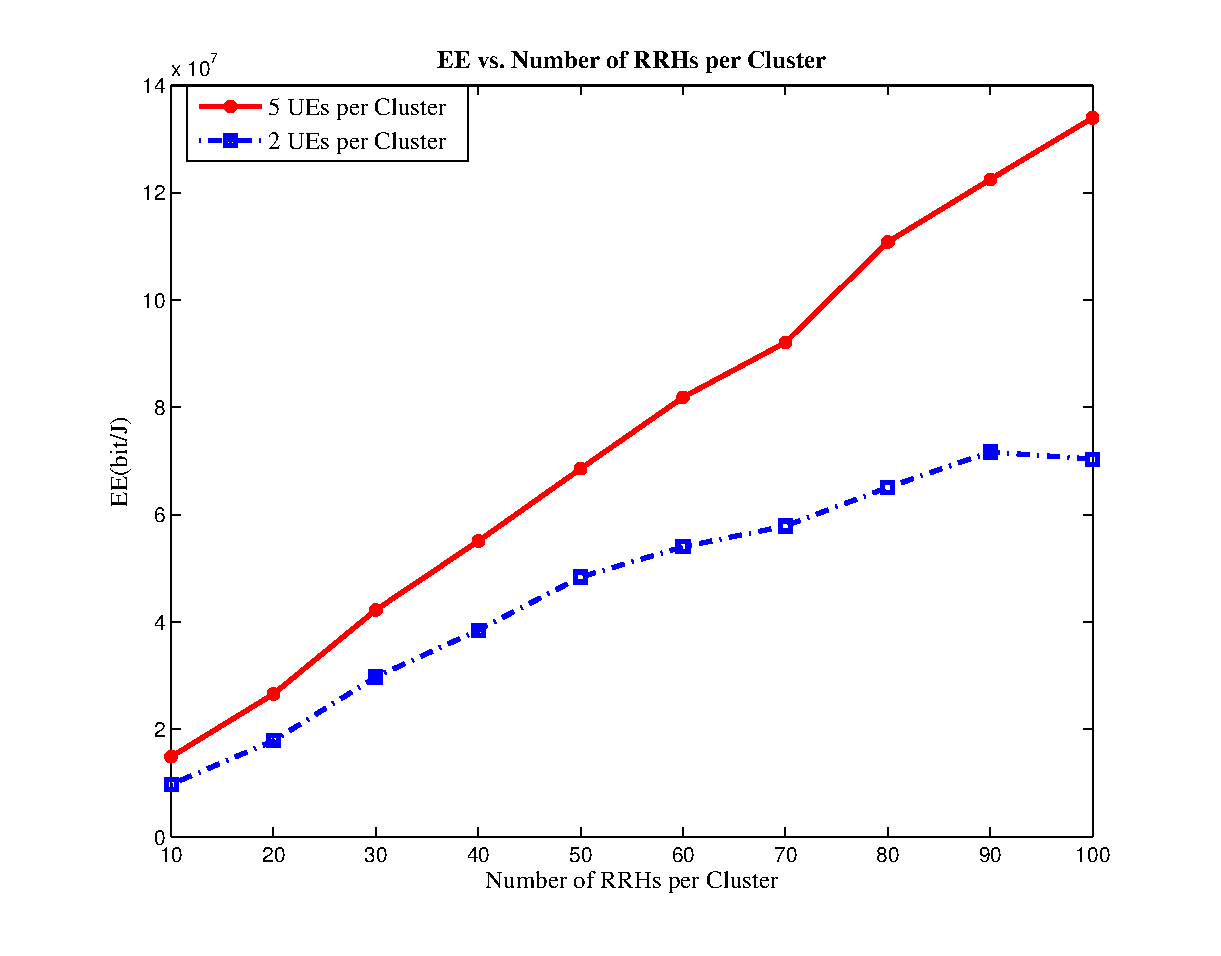
\includegraphics[width=\linewidth, height=12cm]{./fig3/rrh1}
  \caption{
  بازدهی انرژی با توجه به تغییرات تعداد واحدهای رادیویی  در هر خوشه برای توان بهینه برای 
   دو کاربر مختلف
   و پارامترهای جدول \ref{tab:title22}}
  \label{fig:nem1}
\end{figure}
 در شکل \ref{fig:nem1}، بازدهی انرژی سیستم \lr{MIMO C-RAN} بر اساس تعداد واحدهای رادیویی در هر خوشه برای مدل سیستم مورد نظر و برای دو تعداد کاربر متفاوت، رسم شده است. فرض اینجا بر این است که 2 خوشه برای لینک فروسو و دو خوشه برای فراسو وجود دارد.
 همانطور که  شکل  نشان می دهد، با افزایش تعداد واحدهای رادیوی، بازدهی انرژی افزایش می یابد زیرا  در اینجا با افزایش تعداد واحدهای رادیویی، مجموع توان کل افزایش می یابد در نتیجه نرخ انتقال داده نیز بیشتر می گردد و در نتیجه ی آن، بازدهی انرژی نیز افزایش یافته است. همچنین بازدهی انرژی برای تعداد کاربر بیشتر، به دلیل اینکه مجموع نرخ ها بیشتر می گردد، زیادتر می باشد.
 \begin{figure}[H]
  \centering
    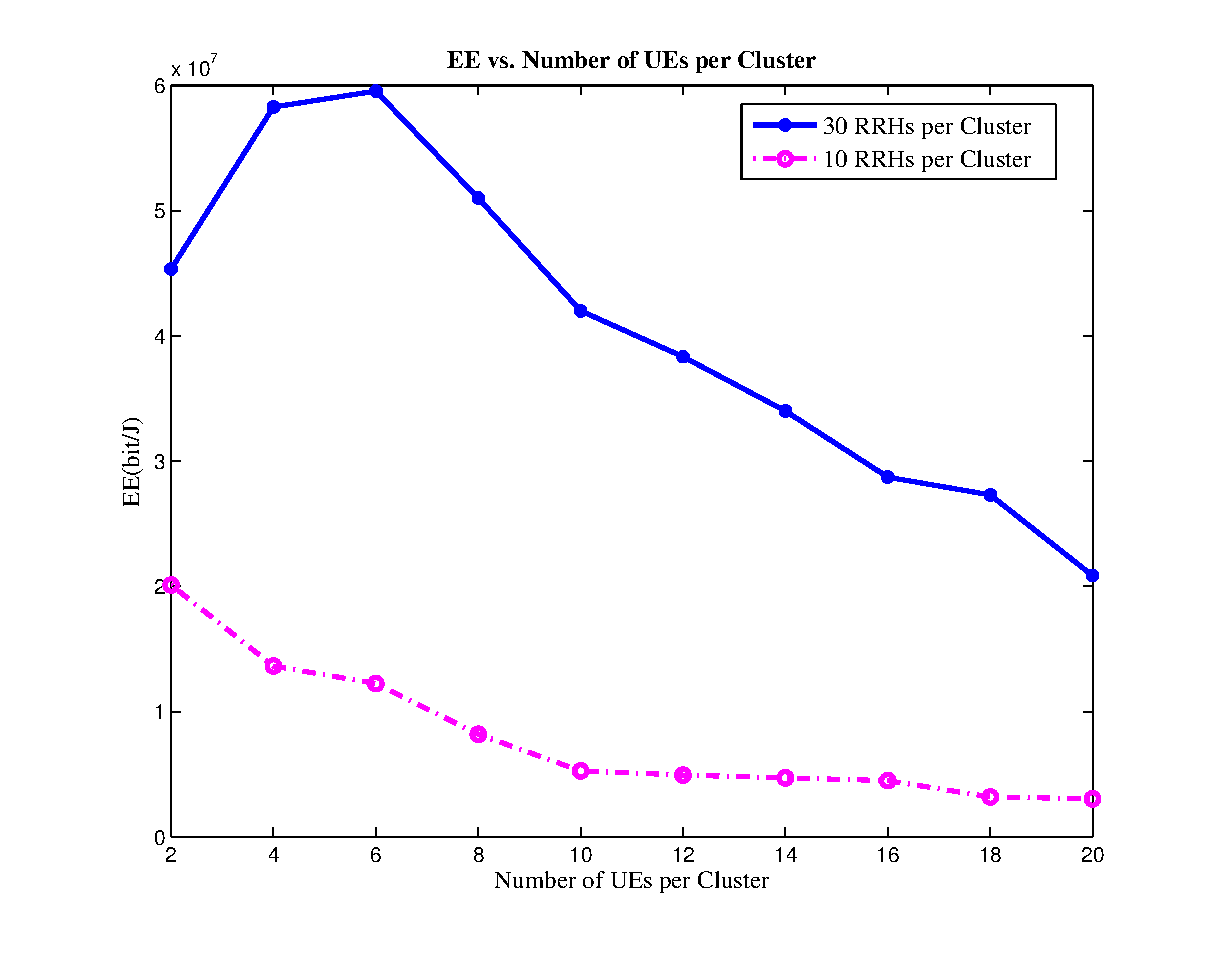
\includegraphics[width=\linewidth]{./fig3/ue4}
  \caption{  بازدهی انرژی با توجه به تغییرات تعداد کاربران در هر خوشه برای توان بهینه برای 
   دو واحد رادیویی مختلف
   و پارامترهای جدول
    \ref{tab:title22} }
  \label{fig:ue4}
\end{figure}

در شکل \ref{fig:ue4}، بازدهی انرژی بر اساس تعداد کاربران در هر خوشه برای مدل سیستم مورد نظر و برای دو تعداد واحد رادیویی متفاوت، رسم شده است. همانطور که  دیده می شود با افزایش تعداد کاربران، در حالتی که 30 واحد رادیویی در هر خوشه داریم، ابتدا به دلیل افزایش کاربران و افزایش مجموع نرخ ها، بازدهی انرژی زیاد شده و در نتیجه ی آن شیب نمودار زیاد می شود ولی از یک مقدار به بعد تداخل بین کاربران افزایش می یابد و منجر به کاهش بازدهی انرژی می گردد. زمانی که تعداد کاربران زیاد نیست، تداخل بین کاربران تاثیر کمی می گذارد و با افزایش کاربران بازدهی انرژی بهبود می یابد ولی زمانی که تعداد کاربران از حدی بیشتر می شود، میزان تداخل به قدری زیاد شده که نرخ انتقال داده کاهش یافته و در نتیجه ی آن، بازدهی انرژی کاهش می یابد. 
در حالتی که  10 واحد رادیویی در هر خوشه داریم، به دلیل اینکه میزان تداخل بین کاربران زیاد است و \lr{SINR} کم است، شیب نمودار از ابتدا منفی است و بازدهی انرژی کم می گردد.
 \begin{figure}[H]
  \centering
    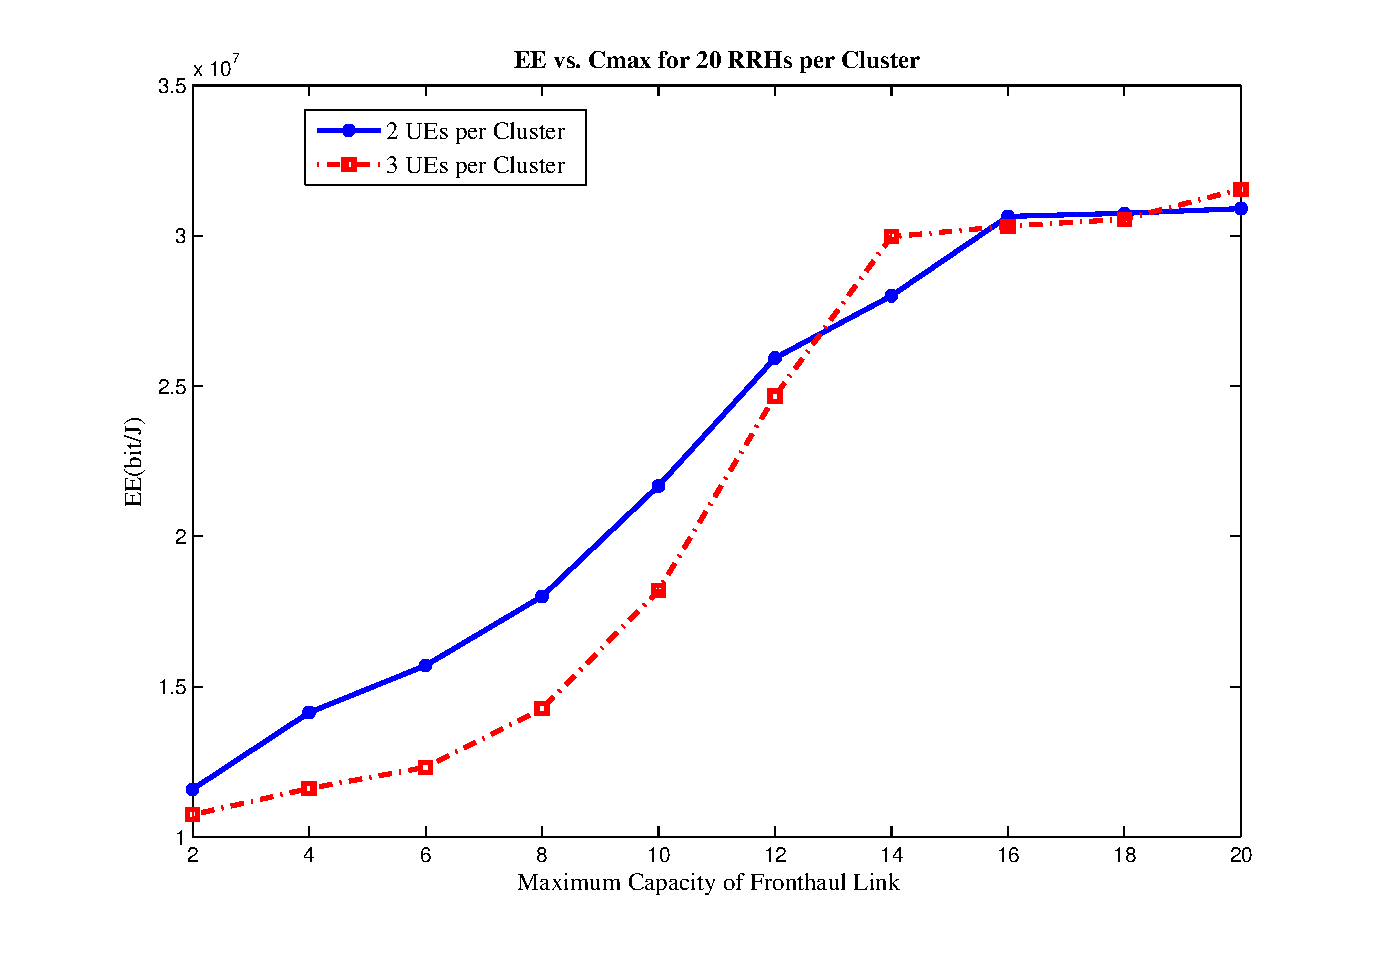
\includegraphics[width=\linewidth]{./fig3/c4}
  \caption{  
  بازدهی انرژی با توجه به تغییرات ظرفیت
   بیشینه ی لینک \lr{fronthaul}
   در هر خوشه برای توان بهینه برای 
   دو تعدا کاربر مختلف
   و پارامترهای جدول
    \ref{tab:title22} }
  \label{fig:c4}
\end{figure}
در شکل \ref{fig:c4}، بازدهی انرژی بر اساس تغییرات ظرفیت
   بیشینه ی لینک \lr{fronthaul} در هر خوشه برای مدل سیستم مورد نظر و برای دو تعداد کاربر متفاوت، رسم شده است.همانطور که  دیده می شود با افزایش این ظرفیت، بازدهی انرژی با شیب زیادی، افزایش یافته ولی از جایی به بعد شیب افزایش کم می گردد زیرا با افزایش بیشینه ی ظرفیت، تعداد بیت های بیشتری می تواند از این لینک عبور کند ولی از یک جایی به بعد، تعداد بیتهایی که در هر ثانیه وجود دارد از نرخ انتقال بیت کمتر است، پس با افزایش نرخ، بازدهی انرژی افزایش پیدا نمی کند. 
\section{نتیجه گیری}
در این فصل، مدل سیستم جدیدی که همزمان شامل چندین خوشه ی لینک فروسو و فراسو است، بیان شده است و همزمان مجموع نرخ های قابل دسترسی بر روی توان کل خوشه های لینک فراسو و فروسو بیشینه شده است و نمودارهای آن را بر حسب تعداد کاربران و واحدهای رادیویی رسم شده اند. با توجه به نمودارها، با افزایش تعداد واحدهای رادیویی توان ارسالی افزایش یافته و بازدهی انرژی بهبود می یابد.  همچنین با افزایش کاربران ابتدا بازدهی انرژی بهبود یافته زیرا مجموع توان افزایش می یابد ولی از حدی به بعد، تاثیر تداخل بین کاربران زیاد شده و بازدهی کاهش می یابد.

% !TeX root=../main.tex
\chapter{بحث و نتیجه‌گیری}
%\thispagestyle{empty} 
\section{مقدمه}
تاکنون شما در پایان‌نامه‌ای که مشغول نوشتن آن هستید، پاسخ چهار سؤال را داده‌اید:
\begin{itemize}
	\item
	چرا تحقیق را انجام دادید؟ (مقدمه)
	\item
	دیگران در این زمینه‌ چه کارهایی کرده‌اند و تمایز کار شما با آنها؟ (مرور ادبیات)
	\item
	چگونه تحقیق را انجام دادید؟ (روش‌ها)
	\item
	چه از تحقیق به دست آوردید؟ (یافته‌ها)
\end{itemize}
حال زمان آن فرا رسیده که با توجه به تمامی مطالب ذکر شده، در نهایت به سؤال آخر پاسخ دهید:
\begin{itemize}
	\item
	چه برداشتی از یافته‌های تحقیق کردید؟ (نتیجه‌گیری)
\end{itemize}
در واقع در این بخش، هدف، پاسخ به این سوال است که چه برداشتی از یافته‌ها کردید و این یافته‌ها چه فایده‌ای دارند؟

نتیجه‌گیری مختصری بنویسید. ارائهٔ داده‌ها، نتایج و یافته‌ها در فصل چهارم ارائه می‌شود. در این فصل تفاوت، تضاد یا تطابق بین نتایج تحقیق با نتایج دیگر محققان باید ذکر شود.
\emph{تفسیر و تحلیل نتایج نباید بر اساس حدس و گمان باشد}،
بلکه باید
\textbf{برمبنای نتایج عملی استخراج‌شده}
از تحقیق و یا
\textbf{استناد به تحقیقات دیگران}
باشد.
با توجه به حجم و ماهیت تحقیق و با صلاحدید استاد راهنما، این فصل می‌تواند تحت عنوانی دیگر بیاید یا به دو فصل جداگانه با عناوین مناسب، تفکیک شود. این فصل فقط باید به جمع‌بندی دست‌آوردهای فصل‌های سوم و چهارم محدود و از ذکر موارد جدید در آن خودداری شود. در عنوان این فصل، به جای کلمهٔ «تفسیر» می‌توان از واژگان «بحث» و «تحلیل» هم استفاده کرد. این فصل شاید مهم‌ترین فصل پایان‌نامه باشد.

در این فصل خلاصه‌ای از یافته‌های تحقیق جاری ارائه می‌شود. این فصل می‌تواند حاوی یک مقدمه، شامل مروری اجمالی بر مراحل انجام تحقیق باشد (حدود یک صفحه). مطالب پاراگراف‌بندی شود و هر پاراگراف به یک موضوع مستقل اختصاص یابد. فقط به ارائهٔ یافته‌ها و دست‌آوردها بسنده شود و
\emph{از تعمیم بی‌مورد نتایج خودداری شود.}
تا حد امکان از ارائهٔ 
\emph{جداول و نمودارها در این فصل اجتناب شود.}
از ارائهٔ 
\emph{عناوین کلی}
در حوزهٔ تحقیق و قسمت پیشنهاد تحقیقات آتی خودداری شود و کاملاً در چارچوب و زمینهٔ مربوط به تحقیق جاری باشد. این فصل حدود ۱۰-۱۵ صفحه است.

\section{محتوا}
به ترتیب شامل موارد زیر است:

\subsection{جمع‌بندی}
خلاصه‌ای از تمام یافته‌ها و دست‌آوردهای تحقیق جاری است.

\subsection{نوآوری}
این قسمت، نوآوری تحقیق را بر اساس یافته‌های آن تشریح می‌کند. که دارای دو بخش اصلی است:
\begin{enumerate}
	\item
	نوآوری تئوری، یعنی تمایز تئوریک کار با کارهای محققین قبلی.
	\item
	نوآوری عملی، یعنی توصیه‌های محقق به صنعت برای بهبود بخشیدن به کارها، بر اساس یافته‌های تحقیق.
\end{enumerate}

\subsection{پیشنهادها}
این بخش، عناوین و موضوعات پیشنهادی را برای تحقیقات آتی،
\emph{بیشتر در زمینهٔ مورد بحث در آینده}
ارائه می‌کند.

\subsection{محدودیت‌ها}
در اینجا انواع محدودیت‌های تحقیق تشریح می‌شوند؛ از جمله، محدودیت‌هایی که کنترل آن از عهده محقق خارج است، مانند انتخاب نوع یافته‌ها؛ و همچنین دیگر محدودیت‌هایی که کنترل آن در دست محقق است، مانند موضوع و محل تحقیق و ... . تأثیر این محدودیت‌ها بر یافته‌های تحقیق در این قسمت شرح داده می‌شوند.

%--------------------------------------------------------------------------appendix( مراجع و پیوست ها)
\chapterfont{\vspace*{-2em}\centering\LARGE}%

\appendix
%\bibliographystyle{plain-fa}
%\bibliographystyle{ieeetr}
%\bibliography{references}
\begin{latin}
\bibliographystyle{IEEEtran}
\renewcommand{\bibname}{\rl{{کتاب‌نامه}\hfill}} 
\bibliography{IEEEabrv,references}
\end{latin}
%\chapter*{‌پیوست}
موضوعات مرتبط با متن گزارش پایان نامه كه در يكی از گروه‌های زير قرار می‌گيرد، در بخش پيوست‌ها آورده شوند:
\begin{enumerate}
\item  اثبات های رياضی يا عمليات رياضی طولانی‌.‌
\item داده و اطلاعات نمونه (های) مورد مطالعه (\lr{Case Study}) چنانچه طولانی باشد‌.‌
\item نتايج كارهای ديگران چنانچه نياز به تفصيل باشد‌.‌

\item مجموعه تعاريف متغيرها و پارامترها، چنانچه طولانی بوده و در متن به انجام نرسيده باشد‌.‌
\end{enumerate}
% براي شماره‌گذاري روابط، جداول و اشكال موجود در پيوست‌ از ساختار متفاوتي نسبت به متن اصلي استفاده مي‌شود كه در زير به‌عنوان نمونه نمايش داده شده‌است. 
% \begin{equation}
%F=ma
%\end{equation}
\section*{کد میپل }
\begin{latin}
\begin{verbatim}

with(DifferentialGeometry):
with(Tensor):
DGsetup([x, y, z], M)
																	frame name: M
a := evalDG(D_x)
																	D_x
b := evalDG(-2 y z D_x+2 x D_y/z^3-D_z/z^2)


\end{verbatim}
\end{latin}
%--------------------------------------------------------------------------dictionary(واژه نامه ها)
%اگر مایل به داشتن صفحه واژه‌نامه نیستید، خط زیر را غیر فعال کنید.
%\parindent=0pt
%%
\chapter*{واژه‌نامه‌ی فارسی به انگلیسی}
\pagestyle{style9}

\addcontentsline{toc}{chapter}{واژه‌نامه‌ی فارسی به انگلیسی}
%%%%%%
\begin{multicols*}{2}

{\bf آ}
\vspace*{3mm}


\farsiTOenglish{اسکالر}{Scalar}


\vspace*{3mm}
{\bf ب}
\vspace*{3mm}

\farsiTOenglish{بالابر}{Lift}


\vspace*{3mm}
{\bf پ}
%%\vspace*{3mm}

\farsiTOenglish{پایا}{Invariant}



\vspace*{3mm}
{\bf ت}
%%\vspace*{3mm}

\farsiTOenglish{ تناظر }{Correspondence}


\vspace*{3mm}
{\bf ث}
%%\vspace*{3mm}

\farsiTOenglish{ثابت‌ساز}{Stabilizer}

\vspace*{3mm}
{\bf ج}
%%\vspace*{3mm}

\farsiTOenglish{جایگشت}{Permutation}



\vspace*{3mm}
{\bf چ}
%%\vspace*{3mm}


\farsiTOenglish{چند جمله‌ای }{Polynomial}

\vspace*{3mm}
{\bf ح}
%%\vspace*{3mm}

\farsiTOenglish{حاصل‌ضرب دکارتی}{Cartesian product}


\vspace*{3mm}
{\bf خ}
%%\vspace*{3mm}

\farsiTOenglish{خودریختی}{Automorphism}

\vspace*{3mm}
{\bf د}
%%\vspace*{3mm}

\farsiTOenglish{درجه}{Degree}


\vspace*{3mm}
{\bf ر}
%%\vspace*{3mm}


\farsiTOenglish{ریزپردازنده}{microprocessor}


\vspace*{3mm}
{\bf ز}
%%\vspace*{3mm}


\farsiTOenglish{زیرمدول}{Submodule}


\vspace*{3mm}
{\bf س}
%%\vspace*{3mm}

\farsiTOenglish{سرشت}{Character}


\vspace*{3mm}
{\bf ص}
%%\vspace*{3mm}

\farsiTOenglish{صادقانه}{Faithful}

\vspace*{3mm}
{\bf ض}
%%\vspace*{3mm}

\farsiTOenglish{ضرب داخلی}{Inner product}

\vspace*{3mm}
{\bf ط}
%%\vspace*{3mm}


\farsiTOenglish{طوقه}{Loop}


\vspace*{3mm}
{\bf ظ}
%%\vspace*{3mm}


\farsiTOenglish{ظرفیت}{Valency}
 
\vspace*{3mm}
{\bf ع}
%%\vspace*{3mm}


\farsiTOenglish{عدم مجاورت}{Nonadjacency}



\vspace*{3mm}
{\bf ف}
%%\vspace*{3mm}

\farsiTOenglish{فضای برداری}{Vector space}



\vspace*{3mm}
{\bf ک}
%%\vspace*{3mm}

\farsiTOenglish{کاملاً تحویل‌پذیر}{Complete reducibility}


\vspace*{3mm}
{\bf گ}
%%\vspace*{3mm}


\farsiTOenglish{گراف}{Graph}



\vspace*{3mm}
{\bf م}
%%\vspace*{3mm}

\farsiTOenglish{ماتریس جایگشتی}{Permutation matrix }


\vspace*{3mm}
{\bf ن}
%%\vspace*{3mm}

\farsiTOenglish{ناهمبند}{Disconnected}


\vspace*{3mm}
{\bf و}
%%\vspace*{3mm}

\farsiTOenglish{وارون‌پذیر}{Invertible}


\vspace*{3mm}
{\bf ه}
%%\vspace*{3mm}

\farsiTOenglish{همبند}{Connected}



\vspace*{3mm}
{\bf ی}
%%\vspace*{3mm}

\farsiTOenglish{یال}{Edge}




\end{multicols*}%
%%%%%%%
\chapter*{ واژه‌نامه‌ی انگلیسی به فارسی}
\pagestyle{style9}
\lhead{\thepage}\rhead{واژه‌نامه‌ی انگلیسی به فارسی}
\addcontentsline{toc}{chapter}{واژه‌نامه‌ی انگلیسی به فارسی}

\LTRmulticolcolumns
\begin{multicols}{2}

{\hfill\bf  \lr{A}}
%%\vspace*{1.5mm}


\englishTOfarsi{Automorphism}{خودریختی}


\vspace*{3mm}
{\hfill\bf   \lr{B}}
%%\vspace*{1.5mm}


\englishTOfarsi{Bijection}{دوسویی}


\vspace*{3mm}
{\hfill\bf   \lr{C}}
%%\vspace*{1.5mm}


\englishTOfarsi{Cycle group}{گروه دوری}

\vspace*{3mm}
{\hfill\bf   \lr{D}}
%%\vspace*{1.5mm}

\englishTOfarsi{Degree}{درجه}


\vspace*{3mm}
{\hfill\bf   \lr{E}}
%%\vspace*{1.5mm}

\englishTOfarsi{Edge}{یال}



\vspace*{3mm}
{\hfill\bf   \lr{F}}
%%\vspace*{1.5mm}


\englishTOfarsi{Function}{تابع}


\vspace*{3mm}
{\hfill\bf   \lr{G}}
%%\vspace*{1.5mm}


\englishTOfarsi{Group}{گروه}

\vspace*{3mm}
{\hfill\bf   \lr{H}}
%%\vspace*{1.5mm}

\englishTOfarsi{Homomorphism}{همریختی}


\vspace*{3mm}
{\hfill\bf   \lr{I}}
%%\vspace*{1.5mm}


\englishTOfarsi{Invariant}{پایا}


\vspace*{3mm}
{\hfill\bf   \lr{L}}
%%\vspace*{1.5mm}

\englishTOfarsi{Lift}{بالابر}



\vspace*{3mm}
{\hfill\bf   \lr{M}}
%%\vspace*{1.5mm}


\englishTOfarsi{Module}{مدول}



\vspace*{3mm}
{\hfill\bf   \lr{N}}
%%\vspace*{1.5mm}

\englishTOfarsi{Natural map}{نگاشت طبیعی}


\vspace*{3mm}
{\hfill\bf   \lr{O}}
%%\vspace*{1.5mm}


\englishTOfarsi{One to One}{یک به یک}



 \vspace*{3mm}
{\hfill\bf   \lr{P}}
%%\vspace*{1.5mm}


\englishTOfarsi{Permutation group}{گروه جایگشتی}


\vspace*{3mm}
{\hfill\bf   \lr{Q}}
%%\vspace*{1.5mm}

\englishTOfarsi{Quotient graph}{گراف خارج‌قسمتی}

 \vspace*{3mm}
{\hfill\bf   \lr{R}}
%%\vspace*{1.5mm}

\englishTOfarsi{Reducible}{تحویل پذیر}


 \vspace*{3mm}
{\hfill\bf   \lr{S}}
%%\vspace*{1.5mm}


\englishTOfarsi{Sequence}{دنباله}



 \vspace*{3mm}
{\hfill\bf   \lr{T}}
%%\vspace*{1.5mm}


\englishTOfarsi{Trivial character}{سرشت بدیهی}


\vspace*{3mm}
{\hfill\bf   \lr{U}}
%%\vspace*{1.5mm}

\englishTOfarsi{Unique}{منحصربفرد}


\vspace*{3mm}
{\hfill\bf   \lr{V}}
%%\vspace*{1.5mm}

\englishTOfarsi{Vector space}{فضای برداری}



\end{multicols}
%--------------------------------------------------------------------------index(نمایه)
%اگر مایل به داشتن صفحه نمایه نیستید، خط زیر را غیر فعال کنید.
\pagestyle{style7}
\printindex
\pagestyle{style7}
%کلمات کلیدی انگلیسی
\latinkeywords{ Cloud Radio Access Network, Multiple-Input Multiple-Output, Energy efficiency, Clusterization, Power allocation, Lagrangian function.}
%چکیده انگلیسی

\en-abstract{
Since more rate and speed is needed in technology, new generation of technology is considered that new concepts such as CRAN, mm wave, Massive MIMO and etc are defined. 
Cloud radio access networks generate a new architechture for 5G that is proposed to enhance both spectral efficiency and energy efficiency. 
The architecture of cran and the difference between this architucture and traditional one is expressed.
Also some system models such as clustering and limited fronthaul capacity is considered. In addition, D2D system in C-RAN is described too.
The optimal power allocation for the downlink and uplink of Multiple-Input Multiple-Output (MIMO) Cloud Radio Access Network (C-RAN) with limited fronthaul capacity in terms of maximizing Energy Efficiency (EE) is investigated. 
In the considered system, in downlink the compressed and precoded message generated by Central Unit (CU) is transmitted to Remote Radio Heads (RRHs) via a fronthaul link with limited capacity, and the RRHs and Users Equipments (UEs) are assumed to be clustered into $S$ cluster sets.
In uplink, the recieved message by RRHs which are clusteres into $S$ clusters, is transmitted through fronthaul link to CU and in CU beamforming vector is applied to the message.
Here, we use an iterative algorithm with Lagrangian function to optimize the EE.
Also both uplink and downlink clusters are considered in a system model and optimization is done for both together.
}
%%%%%%%%%%%%%%%%%%%%% کدهای زیر را تغییر ندهید.

\newpage
\thispagestyle{empty}
\begin{latin}
\section*{\LARGE\centering Abstract}

\een-abstract

\vspace*{.5cm}
{\large\textbf{Key Words:}}\par
\vspace*{.5cm}
\elatinkeywords
\end{latin}
% در این فایل، عنوان پایان‌نامه، مشخصات خود و چکیده پایان‌نامه را به انگلیسی، وارد کنید.
%%%%%%%%%%%%%%%%%%%%%%%%%%%%%%%%%%%%
\baselineskip=.6cm
\begin{latin}

\latinfaculty{Department of Electrical Engineering}


\latintitle{Improveing the performance of Cloud Radio Access Network with distributed cooperation}


\firstlatinsupervisor{Dr. Mohammad Javad Emadi}

%\secondlatinsupervisor{Second Supervisor}

\firstlatinadvisor{Dr. Abbas Mohammadi }

%\secondlatinadvisor{Second Advisor}

\latinname{Mojdeh}

\latinsurname{Karbalaee Motalleb}

\latinthesisdate{Month 6 \& Year 1396}

\latinvtitle
\end{latin}

\end{document}